\documentclass[12pt]{article}
\usepackage[a4paper,margin=19mm,headheight=15pt]{geometry}
\usepackage[T1]{fontenc}
\usepackage{graphicx}
\usepackage{lmodern,microtype,amsmath,amssymb,mathtools,array,longtable,enumitem}
\usepackage[most]{tcolorbox}
\usepackage{fancyhdr,hyperref,bookmark,needspace}
\definecolor{navy}{HTML}{183650}
\definecolor{teal}{HTML}{007D83}
\definecolor{amber}{HTML}{A65F08}
\hypersetup{colorlinks=true,linkcolor=teal,urlcolor=teal}
\pagestyle{fancy}\fancyhf{}\fancyhead[L]{\small MATH6310 | Metric Spaces \& Topology}\fancyhead[R]{\small Sai Vanam}\fancyfoot[C]{\thepage}
\setlength{\parindent}{0pt}\setlength{\parskip}{5pt}
\setlist{nosep,leftmargin=*}
\tcbset{enhanced,breakable,colback=blue!2!white,colframe=navy,boxrule=.6pt,arc=1.5mm,left=3mm,right=3mm,top=2mm,bottom=2mm,before skip=9pt,after skip=9pt,fonttitle=\bfseries}
\newtcolorbox{note}[1]{title={#1}}
\newtcolorbox{method}[1]{title={Method: #1},colframe=teal,colback=teal!3!white}
\newtcolorbox{exam}[1]{title={Exam question: #1},colframe=amber,colback=yellow!5!white}
\newtcolorbox{answer}{title={Worked model answer},colframe=teal,colback=green!2!white}
\newtcolorbox{tip}{title={Exam tips and common mistakes},colframe=amber,colback=orange!3!white}
\newcommand{\R}{\mathbb R}\newcommand{\Q}{\mathbb Q}\newcommand{\N}{\mathbb N}\newcommand{\Z}{\mathbb Z}\newcommand{\C}{\mathbb C}
\newcommand{\cl}[1]{\overline{#1}}\newcommand{\inte}{\operatorname{Int}}\newcommand{\diam}{\operatorname{diam}}\newcommand{\dist}{\operatorname{dist}}\newcommand{\Lip}{\operatorname{Lip}}\newcommand{\norm}[1]{\left\lVert#1\right\rVert}
\newcommand{\topic}[1]{\par\Needspace{50mm}\subsection{#1}}

\linespread{1.12}
\newcommand{\exercise}[2]{\Needspace{45mm}\subsubsection{Exercise #1: #2}}

\renewcommand{\thesection}{\arabic{section}}
\renewcommand{\thesubsection}{\arabic{section}.\arabic{subsection}}
\renewcommand{\thesubsubsection}{\arabic{section}.\arabic{subsection}.\arabic{subsubsection}}
\setcounter{tocdepth}{2}

\usepackage{titlesec}
\titleformat{\section}{\Large\bfseries}{Section \thesection}{1em}{}

\begin{document}
\begin{titlepage}
\vspace*{18mm}
{\Huge\bfseries\color{navy} Metric Spaces\par\& Topology\par}
\vspace{8mm}{\Large MATH6310\par Expanded lecture notes, proofs and worked exercises\par}
\vspace{5mm}{\large Prepared for Sai Vanam}
\vspace{10mm}
\begin{note}{What this guide gives you}
Definitions translated into plain English; slower explanations of proof decisions; theorem hypotheses and proofs; question methods; counterexamples; exam questions with model answers; and a complete worked practice section for all 79 numbered exercises in the supplied lecture sections. Based on the twelve PDFs supplied here and the recovered original Section 1 PDF, including MATH316 papers from 2022--2025.
\end{note}
\begin{note}{Structure and sources}
The guide follows Part I, Sections 0--6, and then Appendices I and II. Section 1 uses the original 26-page PDF recovered from your earlier uploads, so it is now based on the lecture source rather than a reconstruction. Explanations, exam questions and worked exercises are grouped inside their relevant section. Non-examinable and optional topics retain those labels. Any later parts beyond the supplied Part I material are outside this guide's source coverage.

MATH316 is the code on the historical papers; MATH6310 is the code on the 2026 notes. Historical questions are useful practice, not confirmation of your current assessment format. Worked answers here are independently written, not official mark schemes.
\end{note}
\begin{note}{How to use the boxes}
Blue: understand and learn. Teal: a reusable method or model answer. Gold: practise before reading the answer, or check a common mistake. Both appendices, Baire category, and the completion existence/uniqueness proof are identified separately where the supplied notes mark them non-examinable.
\end{note}
\vfill{\small Source notes dated 7 September 2026; appendices dated 10 September 2026.}
\end{titlepage}
\tableofcontents\clearpage

\clearpage
\setcounter{section}{-1}
\section{What is a metric space?}

\topic{Finding the right method quickly}
\begin{method}{Translate the command into a first line}
\begin{tabular}{p{.32\linewidth}p{.61\linewidth}}
\textbf{Question asks you to}\quad & \textbf{Start with}\rule{0pt}{4ex}\\
Verify a metric & Check finiteness, nonnegativity, zero iff equality, symmetry, then triangle inequality.\\[4pt]
Prove $U$ open & ``Let $p\in U$. Choose $r=\cdots>0$. If $d(x,p)<r$, then $x\in U$.''\\[4pt]
Prove $F$ closed & Take $x_n\in F$ with $x_n\to x$ in the ambient space; prove $x\in F$.\\[4pt]
Find closure/boundary & Classify points by whether every ball meets the set, or both set and complement.\\[4pt]
Prove continuity & Find $\delta$, use convergent sequences, or test inverse images of open sets.\\[4pt]
Prove density & Fix any ball $B_r(p)$ and produce a point of the proposed dense set inside it.\\[4pt]
Prove completeness & Start with an arbitrary Cauchy sequence; construct its limit and keep it inside the space.\\[4pt]
Prove compactness & In $\R^n$, use closed and bounded. In general, extract subsequences or use a known compact image/product.\\[4pt]
Apply Banach & Verify nonempty complete space, self-map, uniform contraction constant $q<1$.\\[4pt]
Disprove a universal claim & Give one example and verify both the hypotheses and the failure of the conclusion.
\end{tabular}
\end{method}
\begin{tip}
A proof is a chain of justified statements, not a list of theorem names. State where each assumption enters. For an ``if and only if'', prove both directions. For limits and compactness, explicitly state that the limit belongs to the required set. A diagram can suggest an answer, but arbitrary metric spaces need an argument using distances.
\end{tip}
\begin{note}{Suggested study order}
First learn metric axioms, balls and sequence definitions. Next learn openness, closedness and continuity. Then study completeness and uniform limits. Finally learn sequential compactness and products. Revisit real analysis whenever a proof uses a supremum, an infimum or a subsequence. After each topic, attempt its question before reading the answer; then reproduce the proof with the answer hidden.
\end{note}


\topic{Metric axioms and core examples}
\begin{note}{What a metric means}
A metric is a function $d:S\times S\to[0,\infty)$ satisfying, for all $x,y,z\in S$,
\[d(x,y)=0\iff x=y,\qquad d(x,y)=d(y,x),\qquad d(x,z)\le d(x,y)+d(y,z).\]
Distances must be finite. A metric space is the pair $(S,d)$: the same set with a different metric may have different convergence, boundedness or completeness properties.

Intuition: distance distinguishes points, is independent of direction, and a detour cannot beat the direct distance. Most metric proofs reduce to the triangle inequality.
\end{note}
\begin{method}{Metric verification}
Check the candidate is defined and finite on every pair. Prove definiteness in both directions. Prove symmetry. For the triangle inequality, either apply a known norm inequality, work pointwise then sum/supremise, or split cases for piecewise formulas. To disprove a candidate it suffices to exhibit one failed axiom. For example $d(x,y)=|x-y|^2$ fails with $x=0,y=1,z=2$, since $4>1+1$.
\end{method}
\begin{note}{Discrete metric and counting metric}
The discrete metric is $d(x,y)=0$ for $x=y$ and $1$ otherwise. It works on \emph{any} set. If $x\ne z$, at least one of $x\ne y$ and $y\ne z$ holds, so the right side of the triangle inequality is at least $1$.

For finite subsets $A,B$ of a set,
\[d(A,B)=\#(A\triangle B),\qquad A\triangle B=(A\setminus B)\cup(B\setminus A).\]
This counts the membership changes needed to transform $A$ into $B$. Since
\[A\triangle C\subseteq(A\triangle B)\cup(B\triangle C),\]
cardinality gives the triangle inequality. If the underlying set is infinite, restrict to finite subsets to ensure the formula stays finite.
\end{note}
\begin{exam}{Section 0 Exercises 0.1 and 0.4: model metric proofs}
(a) Prove the discrete metric is a metric. (b) Prove the counting metric satisfies the triangle inequality.
\end{exam}
\begin{answer}
(a) Its values are $0$ and $1$, hence finite and nonnegative. By definition $d(x,y)=0$ exactly when $x=y$. Equality/inequality of points is symmetric, so $d(x,y)=d(y,x)$. Let $x,y,z\in S$. If $x=z$, the left side is zero, so the triangle inequality holds. If $x\ne z$, $x=y=z$ is impossible, so $d(x,y)+d(y,z)\ge1=d(x,z)$. This proves all axioms.

(b) Let $s\in A\triangle C$. Its membership in $A$ and $C$ differs. If its membership in $B$ agrees with $A$, it differs from $C$, so $s\in B\triangle C$. Otherwise $s\in A\triangle B$. Hence the displayed inclusion holds. For finite sets,
\[\#(A\triangle C)\le\#((A\triangle B)\cup(B\triangle C))\le\#(A\triangle B)+\#(B\triangle C).\]
This is precisely $d(A,C)\le d(A,B)+d(B,C)$.
\end{answer}
\begin{note}{Norm metrics and $\ell^p$ examples}
Every norm gives $d(x,y)=\norm{y-x}$. In $\R^n$ or $\C^n$,
\[\norm{x}_p=\left(\sum_{i=1}^n|x_i|^p\right)^{1/p}\ (1\le p<\infty),\qquad \norm{x}_\infty=\max_i|x_i|.\]
$p=1$ is Manhattan distance, $p=2$ Euclidean distance, $p=\infty$ maximum distance. Their unit spheres in $\R^2$ are respectively a diamond, circle and square. For $1<p<2$ the curve $|x|^p+|y|^p=1$ lies between diamond and circle; for $p>2$ it lies between circle and square.

The inequalities
\[\norm{x}_\infty\le\norm{x}_p\le n^{1/p}\norm{x}_\infty\]
show equivalence of these finite-dimensional norms. For $p=1$ sum scalar triangle inequalities; for $p=\infty$ bound every coordinate by the same maximum bound. The general triangle inequality is Minkowski's inequality (Appendix I).
\end{note}
\begin{exam}{2023 Q2(a): norms, metrics and matrices}
Show that a norm induces a metric and give a norm on $M_2(\R)$ with justification.
\end{exam}
\begin{answer}
Set $d(x,y)=\norm{y-x}$. It is finite and nonnegative. Definiteness gives $d(x,y)=0\iff y-x=0\iff x=y$. Homogeneity with scalar $-1$ gives symmetry. Finally,
\[d(x,z)=\norm{z-x}=\norm{(z-y)+(y-x)}\le\norm{z-y}+\norm{y-x}=d(y,z)+d(x,y).\]
On matrices define $\norm{A}=\sum_{i,j=1}^2|a_{ij}|$. The sum is nonnegative and is zero iff all entries vanish. Also $\norm{\lambda A}=|\lambda|\norm{A}$, and
\[\norm{A+B}=\sum_{i,j}|a_{ij}+b_{ij}|\le\sum_{i,j}|a_{ij}|+\sum_{i,j}|b_{ij}|=\norm{A}+\norm{B}.\]
Thus it is a norm. The Frobenius norm is another valid choice, using the Euclidean norm of the four entries.
\end{answer}
\begin{note}{Visual explanation: unit spheres under different norms}
\begin{center}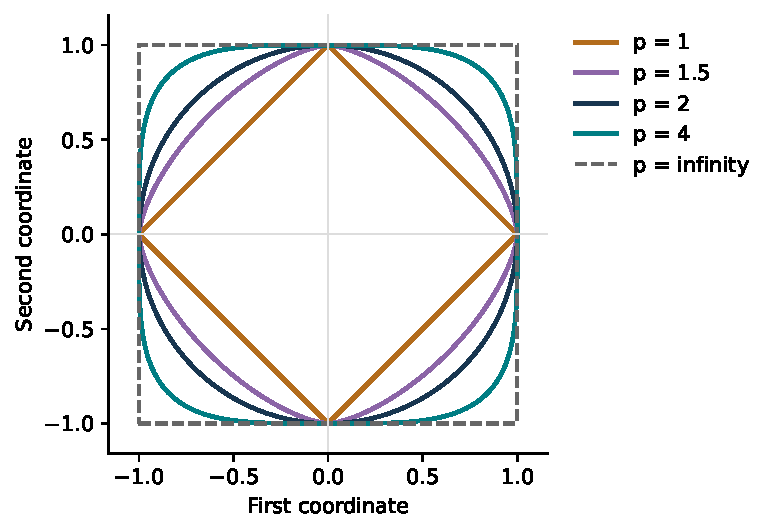
\includegraphics[width=.92\linewidth]{figures/unit_spheres.pdf}\end{center}
Each curve consists of vectors of norm one for a different norm on the same plane. The changing shape is a change of distance rule, not of the underlying points. The unit ball is the region inside its curve; the closed ball also includes the curve. This picture also supports Exercise 3.9.
\end{note}


\topic{Function metrics, Hausdorff distance and unusual metrics}
\begin{note}{Integral and sup metrics on functions}
For continuous real functions on $I=[0,1]$,
\[d_1(f,g)=\int_I|f-g|,\qquad d_{\sup}(f,g)=\sup_{t\in I}|f(t)-g(t)|.\]
The first measures total discrepancy; the second measures worst-case discrepancy. Integral definiteness uses continuity, as proved earlier. For the sup metric, definiteness follows because if the supremum is zero, every pointwise difference is zero. The pointwise inequality
\[|f(t)-h(t)|\le|f(t)-g(t)|+|g(t)-h(t)|\le d_{\sup}(f,g)+d_{\sup}(g,h)\]
gives the triangle inequality upon taking a supremum.

Since $d_1\le d_{\sup}$, uniform convergence implies integral convergence. The converse fails: continuous triangular spikes of height $1$ and support $[0,1/n]$ have integral $1/(2n)$ but sup norm $1$.
\end{note}
\begin{note}{The general sup-metric space $\ell^\infty(S;E)$}
This is the set $F_b(S;E)$ of functions with bounded image, with metric
\[d_{\sup}(f,g)=\sup_{s\in S}d_E(f(s),g(s)).\]
For nonempty $S$, fix $s_0\in S$. Then
\[d(f(s),g(s))\le\diam f(S)+d(f(s_0),g(s_0))+\diam g(S),\]
so the supremum is finite. Metric axioms follow pointwise and then by taking the supremum. For empty $S$ there is a single function; give that singleton its zero metric. No vector-space structure of $E$ is required.
\end{note}
\begin{note}{Hausdorff distance: distance between whole sets}
For nonempty closed bounded subsets of $\R^n$, put
\[d_H(A,B)=\max\left\{\sup_{a\in A}\dist(a,B),\ \sup_{b\in B}\dist(b,A)\right\}.\]
Equivalently, it is the infimum of $\delta\ge0$ such that each set lies in the other's $\delta$-fattening. Nonemptiness makes the distance-to-set expression meaningful; boundedness ensures finiteness; closedness ensures zero distance means equality.

If $A\subseteq B$, then $A_\delta\subseteq B_\delta$. If $x\in(A_\gamma)_\delta$, choose $y\in A_\gamma$ with $d(x,y)\le\delta$ and $a\in A$ with $d(y,a)\le\gamma$. Then $d(x,a)\le\gamma+\delta$, so $(A_\gamma)_\delta\subseteq A_{\gamma+\delta}$ (for the fattenings defined by existence in the supplied notes).
\end{note}
\begin{exam}{Section 0 Exercise 0.6: Hausdorff triangle inequality}
Deduce $d_H(A,C)\le d_H(A,B)+d_H(B,C)$ from the fattening properties.
\end{exam}
\begin{answer}
Let $a=d_H(A,B)$ and $b=d_H(B,C)$, and fix $\varepsilon>0$. By the definition of infimum and monotonicity of fattening, choose admissible radii $r<a+\varepsilon$ and $s<b+\varepsilon$ such that $A\subseteq B_r$, $B\subseteq A_r$, $B\subseteq C_s$, $C\subseteq B_s$. Then
\[A\subseteq B_r\subseteq(C_s)_r\subseteq C_{r+s},\qquad C\subseteq B_s\subseteq(A_r)_s\subseteq A_{r+s}.\]
Thus $d_H(A,C)\le r+s<a+b+2\varepsilon$. Let $\varepsilon\downarrow0$ to obtain the triangle inequality. The small error terms avoid assuming an infimum is attained.
\end{answer}
\begin{note}{TGV metrics and pullbacks}
On $\R^2$, the TGV metric is $d_T(x,y)=\norm{x}_2+\norm{y}_2$ for distinct points and zero on the diagonal. The radial variant uses $\norm{x-y}_2$ when $x,y$ are linearly dependent, and the sum of norms otherwise.

For $d_T$, if the intermediate point equals an endpoint the triangle inequality is equality; otherwise the right side includes the norms of both endpoints and an additional $2\norm{y}$. For the radial variant, distances are lengths of shortest permitted paths along lines through the origin. Algebraically: if the endpoints are dependent, each leg dominates Euclidean distance. If the endpoints are independent and both legs are independent, the result is immediate. If exactly one leg is dependent, use $\norm{x}\le\norm{x-y}+\norm{y}$ (or the analogous inequality for the other endpoint). Both legs cannot be dependent with $y\ne0$ unless the endpoints are dependent. With $y=0$, both legs sum to $\norm{x}+\norm{z}$.

An injective map $\phi:A\to(E,d)$ defines a pullback metric $d_A(x,y)=d(\phi(x),\phi(y))$. Injectivity is needed for definiteness. Example:
\[d_{NS}(x,y)=|\arctan x-\arctan y|\quad(x,y\in\R).\]
This is bounded by $\pi$ and is isometric to the usual interval $(-\pi/2,\pi/2)$. It is not induced by a norm on $\R$, because a norm would make $d(0,n)=n\norm{1}$ unbounded.
\end{note}
\begin{exam}{Additional practice: why continuity depends on the metric}
For the TGV metric on $\R$, show that the identity from TGV to the usual metric is Lipschitz, but the reverse identity is continuous only at zero.
\end{exam}
\begin{answer}
For distinct $x,y$, $|x-y|\le|x|+|y|=d_T(x,y)$; on the diagonal both distances are zero. Thus the identity to the usual metric is $1$-Lipschitz. At zero $d_T(x,0)=|x|$, so the reverse identity is continuous there. If $a\ne0$, take $x_n=a+1/n$. Then $x_n\to a$ in the usual metric but $d_T(x_n,a)=|a+1/n|+|a|\to2|a|>0$. Therefore the reverse identity is not continuous at $a$ and the metrics are not topologically equivalent.
\end{answer}


\topic{Proof clinic: Quantifiers: what the examiner is asking you to construct}
\begin{note}{Read a definition as a conversation}
For openness, someone gives you a point $p\in U$. You must answer with a positive radius $r$, and then prove that \emph{every} point inside that ball stays in $U$. Your radius may depend on $p$. This is why an interval such as $(0,1)$ is open even though points near its endpoints need very small radii.

For convergence, someone gives you an accuracy $\varepsilon>0$. You must answer with a cutoff $N$, after which \emph{every} term is close enough. A finite number of failures before $N$ does not matter. The cutoff may depend on $\varepsilon$, but not on the later index $n$.

For Cauchyness, after your cutoff all pairs of terms must be close. You do not choose a separate cutoff for each later pair. That is why showing $d(x_n,x_{n+1})\to0$ does not suffice: it controls adjacent terms, rather than arbitrary pairs.

For sequential compactness, you are given any sequence and must extract a suitable subsequence. You do not need the original sequence itself to converge. For example $(-1)^n$ lies in the compact interval $[-1,1]$ but does not converge; its even subsequence is constantly $1$.
\end{note}
\begin{exam}{Additional practice: spot the quantifier error}
A student argues: ``For each $n$, choose $N=n+1$. Then all terms after $N$ are late, so the sequence converges.'' What is missing?
\end{exam}
\begin{answer}
There is no proposed limit and no bound on the distance to it. More fundamentally, the required cutoff must be chosen after the tolerance but before the universally quantified later index. Writing $N=n+1$ makes the cutoff depend on the very index it is supposed to control. A valid proof must name a point $a$ and, for each $\varepsilon$, choose one $N(\varepsilon)$ such that $d(x_n,a)<\varepsilon$ holds for every $n\ge N(\varepsilon)$.
\end{answer}


\topic{Proof clinic: A manageable routine for each topic}
\begin{note}{Use the expanded notes actively}
\textbf{First pass:} read the intuitive explanation and one example. Say the idea aloud in ordinary words. For instance, complete means that sequences whose terms become mutually close do not run into missing points.

\textbf{Second pass:} write the formal definition from memory. Check every quantifier and where the metric is evaluated. Then reconstruct the proof's main estimate before reading the intermediate steps.

\textbf{Third pass:} attempt a numbered lecture exercise. Read only the method box if stuck. After checking the solution, close the notes and write the argument again in your own words.

\textbf{Fourth pass:} attempt a past-paper question on the same topic. Give reasons for each implication and verify every theorem hypothesis. Collect an example and a counterexample beside the definition.

The objective is to recognise the structure of a new question: local-radius construction, sequence-limit argument, infimum approximation, uniform-error estimate, subsequence extraction, or fixed-point verification. Those structures recur across the whole supplied module material.
\end{note}


\topic{Worked lecture exercises}
\begin{note}{How to read this workbook}
Each exercise starts with the task, then gives the reason for the chosen method, a complete solution and a reusable lesson. The statements are restated in a compact form; consult the original exercise sheet for the original wording. Try the question first. If stuck, read the method box, cover the solution, and try again.
\end{note}
\exercise{0.1}{The discrete metric}
\begin{exam}{Lecture exercise}
For any set $S$, put $d(x,y)=0$ if $x=y$ and $d(x,y)=1$ otherwise. Prove $d$ is a metric.
\end{exam}
\begin{method}{Use the two possible values}
The first axioms follow directly from the definition. The triangle inequality only needs thought when its left side is $1$. Ask whether both terms on the right could then be zero.
\end{method}
\begin{answer}
The function is defined for every pair and takes finite nonnegative values. By construction, $d(x,y)=0$ exactly when $x=y$. Since $x=y$ iff $y=x$, the definition gives $d(x,y)=d(y,x)$.

Fix $x,y,z\in S$. If $x=z$, then $d(x,z)=0$ and the right side of the triangle inequality is nonnegative. If $x\ne z$, then at least one of $x\ne y$, $y\ne z$ holds: otherwise $x=y=z$, a contradiction. Therefore at least one of $d(x,y),d(y,z)$ is $1$, giving
\[d(x,z)=1\le d(x,y)+d(y,z).\]
Thus the triangle inequality holds for every triple, and $d$ is a metric.
\end{answer}
\begin{tip}
Do not assume the three points are distinct. A metric axiom must hold for repeated points too. Separating the case $x=z$ handles this safely.
\end{tip}
\exercise{0.2}{Why integral distance distinguishes continuous functions}
\begin{exam}{Lecture exercise}
For continuous $h:[0,1]\to\R$, prove $\int_0^1|h(t)|\,dt=0\Rightarrow h=0$.
\end{exam}
\begin{method}{Prove the contrapositive}
If $h$ is nonzero somewhere, continuity prevents its absolute value from dropping immediately to zero. It stays above a positive height on an interval of positive length; that creates positive area.
\end{method}
\begin{answer}
Suppose $h\ne0$. Then $h(p)\ne0$ for some $p\in[0,1]$. Let $c=|h(p)|>0$. By continuity there is $\delta>0$ such that
\[t\in[0,1],\ |t-p|<\delta\quad\Rightarrow\quad |h(t)-h(p)|<c/2.\]
The reverse triangle inequality gives
\[|h(t)|\ge |h(p)|-|h(t)-h(p)|>c/2.\]
The relative neighbourhood $[0,1]\cap(p-\delta,p+\delta)$ contains a closed interval $J$ of positive length, including when $p$ is an endpoint. Since $|h|\ge0$ everywhere,
\[\int_0^1|h|\ge\int_J|h|\ge(c/2)|J|>0.\]
Thus nonzero $h$ forces positive integral. Its contrapositive is the requested implication. Applied to $h=f-g$, it proves definiteness of $d_1$ on continuous functions.
\end{answer}
\begin{tip}
The integrand being nonnegative is not enough for pointwise vanishing: a function supported at one point has zero integral. Continuity supplies the interval on which the positive lower bound holds.
\end{tip}
\exercise{0.3}{The sup metric}
\begin{exam}{Lecture exercise}
For $f,g\in C([0,1];\R)$, let $d_{\sup}(f,g)=\sup_t|f(t)-g(t)|$. Prove definiteness and triangle inequality.
\end{exam}
\begin{answer}
Continuous functions on the compact interval are bounded, so the supremum is finite. If $d_{\sup}(f,g)=0$, then for every $t$,
\[0\le |f(t)-g(t)|\le d_{\sup}(f,g)=0.\]
Therefore $f(t)=g(t)$ for every $t$, so $f=g$. Conversely $f=g$ makes every difference zero, giving $d_{\sup}(f,g)=0$.

For any continuous $h$ and any fixed $t$,
\begin{align*}
|f(t)-h(t)|&\le |f(t)-g(t)|+|g(t)-h(t)|\\
&\le d_{\sup}(f,g)+d_{\sup}(g,h).
\end{align*}
The last bound does not depend on $t$. It is therefore an upper bound for all the numbers whose supremum defines $d_{\sup}(f,h)$. Consequently
\[d_{\sup}(f,h)\le d_{\sup}(f,g)+d_{\sup}(g,h).\]
\end{answer}
\begin{method}{The transferable step}
First bound every pointwise expression by a common constant; then take the supremum. A supremum is a least upper bound, so it is at most any upper bound you have proved.
\end{method}
\exercise{0.4}{Counting distance}
\begin{exam}{Lecture exercise}
For finite sets $A,B$, let $d(A,B)=\#(A\triangle B)$. Prove the triangle inequality.
\end{exam}
\begin{answer}
Fix a third finite set $C$. We prove
\[A\triangle C\subseteq(A\triangle B)\cup(B\triangle C).\]
Take $s\in A\triangle C$. If $s\in A$ and $s\notin C$, either $s\in B$, giving $s\in B\setminus C$, or $s\notin B$, giving $s\in A\setminus B$. If instead $s\in C$ and $s\notin A$, either $s\in B$, giving $s\in B\setminus A$, or $s\notin B$, giving $s\in C\setminus B$. In every case $s$ belongs to the union on the right.

Cardinality is monotone under inclusion, and the size of a finite union is at most the sum of the sizes. Hence
\begin{align*}
d(A,C)&=\#(A\triangle C)\\
&\le\#((A\triangle B)\cup(B\triangle C))\\
&\le\#(A\triangle B)+\#(B\triangle C)=d(A,B)+d(B,C).
\end{align*}
\end{answer}
\begin{note}{A concrete check}
For $A=\{1,2\}$, $B=\{2,3\}$ and $C=\{3,4\}$, the three distances are $2,2,4$, so the triangle inequality is equality. The proof must work for all sets, but a numerical example helps check the interpretation.
\end{note}
\exercise{0.5}{TGV and radial TGV triangle inequalities}
\begin{exam}{Lecture exercise}
Write $\norm{\cdot}=\norm{\cdot}_2$. On $\R^2$ define
\[d_T(x,z)=\begin{cases}0,&x=z,\\\norm{x}+\norm{z},&x\ne z,\end{cases}\]
and define $d_R(x,z)=\norm{x-z}$ when $x,z$ are linearly dependent, and $\norm{x}+\norm{z}$ otherwise. Prove the triangle inequality for both.
\end{exam}
\begin{method}{Split by the formula for the left side}
For the radial metric, dependent endpoints use Euclidean triangle inequality. For independent endpoints, study whether each leg of the detour is dependent. The zero intermediate point needs its own sentence.
\end{method}
\begin{answer}
For $d_T$, fix $x,y,z$. If $x=z$, the left side is zero. If $y=x$ or $y=z$, the inequality is equality. In the remaining case $x\ne z$ and $y$ is different from both, so
\[d_T(x,y)+d_T(y,z)=\norm{x}+2\norm{y}+\norm{z}\ge\norm{x}+\norm{z}=d_T(x,z).\]

For $d_R$, first note that $d_R(u,v)\ge\norm{u-v}$ in every case, by the Euclidean triangle inequality.

If $x,z$ are dependent, then
\[d_R(x,z)=\norm{x-z}\le\norm{x-y}+\norm{y-z}\le d_R(x,y)+d_R(y,z).\]
Now suppose $x,z$ are independent. Then $d_R(x,z)=\norm{x}+\norm{z}$. If $y=0$, the two legs have sum $\norm{x}+\norm{z}$, so the result holds. Assume $y\ne0$.

If both pairs $(x,y)$ and $(y,z)$ are independent, their distances sum to $\norm{x}+2\norm{y}+\norm{z}$, which is large enough. If $x,y$ are dependent and $y,z$ independent, then
\[d_R(x,y)+d_R(y,z)=\norm{x-y}+\norm{y}+\norm{z}\ge\norm{x}+\norm{z}.\]
If $x,y$ are independent and $y,z$ dependent, use $\norm{z}\le\norm{z-y}+\norm{y}$ instead. Finally both pairs cannot be dependent when $y\ne0$: each endpoint would be a scalar multiple of $y$, making $x,z$ dependent. These cases exhaust all possibilities.
\end{answer}
\begin{tip}
The metric is piecewise defined, so ``by triangle inequality'' alone hides the main difficulty. State which branch applies and which Euclidean inequality justifies that branch.
\end{tip}
\exercise{0.6}{Fattenings and Hausdorff triangle inequality}
\begin{exam}{Lecture exercise}
For $A_\delta=\{x:\exists a\in A,\ \norm{x-a}_2\le\delta\}$, prove monotonicity in $A$, prove $(A_\gamma)_\delta\subseteq A_{\gamma+\delta}$, then deduce the Hausdorff triangle inequality.
\end{exam}
\begin{answer}
If $A\subseteq B$ and $x\in A_\delta$, a witness $a\in A$ to $\norm{x-a}\le\delta$ also belongs to $B$. Hence $x\in B_\delta$, proving $A_\delta\subseteq B_\delta$.

If $x\in(A_\gamma)_\delta$, choose $y\in A_\gamma$ with $\norm{x-y}\le\delta$, then $a\in A$ with $\norm{y-a}\le\gamma$. Thus $\norm{x-a}\le\norm{x-y}+\norm{y-a}\le\delta+\gamma$, so $x\in A_{\gamma+\delta}$.

Let $A,B,C$ be nonempty closed bounded Euclidean sets and let $h=d_H(A,B)$, $k=d_H(B,C)$. Fix $\varepsilon>0$. Choose admissible radii $r<h+\varepsilon$ and $s<k+\varepsilon$. This means $A\subseteq B_r$, $B\subseteq A_r$, $B\subseteq C_s$ and $C\subseteq B_s$. Then
\[A\subseteq B_r\subseteq(C_s)_r\subseteq C_{r+s},\qquad C\subseteq B_s\subseteq(A_r)_s\subseteq A_{r+s}.\]
Therefore $r+s$ is an admissible radius between $A,C$, giving
\[d_H(A,C)\le r+s<h+k+2\varepsilon.\]
Letting $\varepsilon\downarrow0$ proves $d_H(A,C)\le d_H(A,B)+d_H(B,C)$.
\end{answer}
\begin{tip}
The set inclusion is one-sided; equality is unnecessary. The $\varepsilon$ terms avoid assuming that the infimum in the Hausdorff definition has an admissible minimising radius.
\end{tip}

\clearpage
\setcounter{section}{0}
\section{Sets, functions and countability}
\begin{note}{Source and learning route}
This section follows the original Section 1 lecture PDF dated 7 September 2026, recovered from your earlier uploads. Its order is: sets and choice; functions and images; equivalence relations and partitions; countability and Cantor's theorem; then optional partial orders and Zorn's lemma. These ideas provide the language for all later metric-space proofs.
\end{note}
\topic{Sets, families, products and the axiom of choice}
\begin{note}{The basic objects}
$A\subseteq S$ means every member of $A$ belongs to $S$. A proper subset also satisfies $A\ne S$. The power set $\mathcal P(S)$ is the set of all subsets of $S$; for example $\mathcal P(\{a,b\})=\{\varnothing,\{a\},\{b\},\{a,b\}\}$.

For a family $\mathcal A$ of subsets of a universe $S$, membership in $\bigcup\mathcal A$ means membership in at least one member, whereas membership in $\bigcap\mathcal A$ means membership in every member. The empty union is $\varnothing$; the empty intersection is $S$. The latter convention depends on the specified universe.
\[A\cap\bigcup\mathcal A=\bigcup_{B\in\mathcal A}(A\cap B),\qquad A\setminus\bigcap\mathcal A=\bigcup_{B\in\mathcal A}(A\setminus B).\]
Prove identities by writing out what it means for an arbitrary point to belong to each side.
\end{note}
\begin{note}{Products and choice}
$\prod_{i\in I}S_i$ consists of indexed families $x=(x_i)_{i\in I}$ with $x_i\in S_i$. Equality means equality in every coordinate. If $I=\N$, these are sequences; if every factor equals $S$, write $S^I$. The empty product contains one empty family. A product with an empty factor is empty.

The axiom of choice says an arbitrary family of nonempty sets has nonempty product. Equivalently there is a choice function selecting one element from each member. A selection from each fibre of a surjection is one place this enters the notes. It does not say that the selection rule is unique.
\end{note}
\topic{Functions, restrictions, inverses and images}
\begin{note}{A function has three ingredients}
Specify a domain, codomain, and one output in the codomain for each input. The range is the outputs actually attained, so it need not equal the codomain. Identity maps, inclusion maps, constant maps, coordinate projections and indicator functions are fundamental examples. An indicator $1_A:S\to\{0,1\}$ is one on $A$ and zero elsewhere in $S$.

For $f:S\to T$ and $g:T\to U$, $(g\circ f)(s)=g(f(s))$. Composition is associative but generally not commutative. Restricting $f$ to $A\subseteq S$ reduces its domain. Extending it reverses that operation. Co-restricting its codomain to $B$ is permitted when the entire range lies in $B$.

There is exactly one function from $\varnothing$ to any $T$, and no function from a nonempty set to $\varnothing$. If finite sets have $n$ domain points and $m$ codomain points, there are $m^n$ functions.
\end{note}
\begin{note}{Injectivity, surjectivity and inverses}
Injective means $f(x)=f(y)\Rightarrow x=y$. Surjective means every target value is attained. Bijective means both. The same squaring rule is not injective on $\R$, but is injective on $[0,\infty)$; changing the codomain also changes surjectivity.

A left inverse satisfies $g\circ f=\mathrm{id}_S$, which forces $f$ injective. Conversely an injection with nonempty domain has a left inverse: invert on the range and send all other target points to one fixed domain point. The empty-domain exception is important.

A right inverse satisfies $f\circ h=\mathrm{id}_T$, which forces surjectivity. Conversely choose one point in each fibre $f^{-1}[\{t\}]$ to obtain a right inverse of a surjection, using choice. A bijection has a two-sided inverse. If $g$ is a left inverse and $h$ a right inverse, associativity gives
\[g=g\circ(f\circ h)=(g\circ f)\circ h=h.\]
Hence a two-sided inverse is unique.
\end{note}
\begin{note}{Images and preimages}
$f[A]=\{f(a):a\in A\}$ and $f^{-1}[B]=\{s:f(s)\in B\}$. The notation $f^{-1}[B]$ does not assume that $f$ has an inverse function.

Images preserve unions and satisfy $f[A\cap B]\subseteq f[A]\cap f[B]$, possibly strictly. Preimages preserve unions, intersections and complements exactly. Always $A\subseteq f^{-1}[f[A]]$, while $f[f^{-1}[B]]=B\cap f[S]$.
\end{note}
\topic{Equivalence relations, partitions and canonical factorisation}
\begin{note}{Equivalence classes group indistinguishable elements}
An equivalence relation is reflexive, symmetric and transitive. Its class $[a]=\{x:x\sim a\}$ contains $a$, and two classes are either identical or disjoint. The set of classes is $S/{\sim}$, and $q(s)=[s]$ is the surjective quotient map.

A partition is a family of nonempty disjoint subsets whose union is $S$. Equivalence classes form a partition: reflexivity covers every point, and symmetry/transitivity show that intersecting classes coincide. Conversely a partition defines $x\sim y$ when they lie in the same block. Coverage gives reflexivity; sharing a block gives symmetry; the uniqueness of the block containing an intermediate point gives transitivity. These constructions undo one another.

Congruence modulo an integer $p\ge2$ groups integers into residue classes. Equality gives singleton classes; the full relation gives one class. The empty relation on a nonempty set is symmetric and transitive but not reflexive.
\end{note}
\begin{note}{Every function factors through its fibres}
For $f:S\to T$, define $x\sim_f y$ iff $f(x)=f(y)$. This is an equivalence relation. The formula $\widetilde f([x])=f(x)$ defines a bijection from $S/{\sim_f}$ to $f[S]$: equivalent representatives have equal outputs, equal outputs give equal classes, and every range value is attained. With $i:f[S]\hookrightarrow T$,
\[f=i\circ\widetilde f\circ q.\]
Thus every map is a surjection onto its classes, followed by a bijection onto its range, followed by an inclusion into the codomain. This pattern later explains quotient metrics and algebraic isomorphism theorems.
\end{note}
\topic{Countability, diagonalisation and comparing sizes}
\begin{note}{Countability rules and how they are proved}
Countable means admitting an injection into $\N$ and includes finite sets. A nonempty set is countable iff it admits a surjection from $\N$. A countably infinite set admits a bijection with $\N$: inject it into $\N$, then enumerate its infinite image in increasing order using well-ordering.

Finite products of countable sets are countable. For example $(n_1,\ldots,n_k)\mapsto p_1^{n_1}\cdots p_k^{n_k}$ injects $\N^k$ into $\N$ by unique prime factorisation. The rationals are countable because $(m,n)\mapsto m/n$ maps countable $\Z\times\N$ onto $\Q$.

A countable union of countable sets is countable: after ignoring empty sets, enumerate each set, and use a two-index list to cover the union. Since $\N^2$ is countable, the combined list is countable. This does not apply to infinite products: $\{0,1\}^{\N}$ is uncountable.
\end{note}
\begin{exam}{Cantor's theorem: model proof}
Prove there is no surjection $f:S\to\mathcal P(S)$.
\end{exam}
\begin{answer}
For any proposed $f$, define $D=\{s\in S:s\notin f(s)\}$. If $f$ were surjective, some $x\in S$ would satisfy $f(x)=D$. Then $x\in D$ iff $x\notin f(x)$ iff $x\notin D$, a contradiction. Hence no such surjection exists. Equivalently, no injection $\mathcal P(S)\to S$ exists. Using the bijection between subsets and indicator functions gives the corresponding result for $\{0,1\}^S$. In particular binary sequence space is uncountable.
\end{answer}
\begin{note}{Schroder--Bernstein theorem: know the statement}
If there is an injection $S\to T$ and an injection $T\to S$, then a bijection $S\to T$ exists. The source notes require knowledge of the theorem but mark its proof non-examinable. It lets you compare sizes without explicitly writing the final bijection. Do not confuse the two arbitrary injections with mutually inverse maps; they need not be inverses.
\end{note}
\topic{Partial orders and Zorn's lemma: optional self-study}
\begin{note}{Order terminology and the maximal-element principle}
A partial order is reflexive, antisymmetric and transitive. Antisymmetry means $x\le y$ and $y\le x$ imply $x=y$; this differs from symmetry. A total order additionally makes every pair comparable. A strict order is asymmetric and transitive; a strict total order has trichotomy.

A chain is a subset of mutually comparable elements. An upper bound dominates every element of a subset. A maximal element has no strictly larger element, but need not dominate all elements of the whole set. For example distinct singleton sets are both maximal in the collection of singleton subsets ordered by inclusion.

Zorn's lemma says that a partially ordered set in which every chain has an upper bound has a maximal element. It is equivalent to the axiom of choice. For linearly independent subsets of a vector space ordered by inclusion, the union of a chain is independent because any finite proposed dependence lies in one chain member. Zorn then gives a maximal independent set, which spans and hence is a basis. Partial functions ordered by extension give another important example: a chain has a union function because its members agree wherever their domains overlap. This explains the extension argument in Appendix II. The source labels this order-theory subsection non-examinable.
\end{note}
\topic{Worked lecture exercises 1.1--1.19}
\exercise{1.1}{Inclusion and symmetric difference}
\begin{exam}{Lecture exercise}
Prove $A\subseteq B\iff A\cap B=A\iff A\cup B=B$, and identify the symmetric difference.
\end{exam}
\begin{answer}
If $A\subseteq B$, intersecting with $B$ removes nothing from $A$ and adjoining $A$ adds nothing to $B$, proving both equalities. Conversely $A=A\cap B$ puts every member of $A$ in $B$; and $A\cup B=B$ also puts each member of $A$ in $B$. Thus either equality gives inclusion.

A point lies in $(A\cup B)\setminus(A\cap B)$ iff it belongs to at least one of $A,B$ but not both, equivalently it lies in $(A\setminus B)\cup(B\setminus A)$. A Venn diagram shades the two nonoverlapping outer parts and leaves the common lens unshaded.
\end{answer}
\exercise{1.2}{Distributivity and De Morgan}
\begin{exam}{Lecture exercise}
Prove $A\cap\bigcup\mathcal C=\bigcup_{C\in\mathcal C}(A\cap C)$ and $A\setminus\bigcap\mathcal C=\bigcup_{C\in\mathcal C}(A\setminus C)$.
\end{exam}
\begin{answer}
For the first identity, $x$ belongs to the left iff $x\in A$ and there exists $C\in\mathcal C$ with $x\in C$, iff there exists $C\in\mathcal C$ with $x\in A\cap C$, which is membership on the right.

For the second, $x$ belongs to the left iff $x\in A$ and not every $C\in\mathcal C$ contains $x$, iff some $C\in\mathcal C$ satisfies $x\in A$ and $x\notin C$, iff $x$ lies on the right. The empty-family conventions make these identities valid in that case too.
\end{answer}
\exercise{1.3}{Counting maps}
\begin{exam}{Lecture exercise}
For $S=\{1,2\}$ and $T=\{1,2,3\}$, count injections $S\to T$, surjections $S\to T$ and surjections $T\to S$.
\end{exam}
\begin{answer}
An injection has $3$ choices for the first output and $2$ remaining choices for the second, giving $6$. No function from two points can attain three different outputs, so there are zero surjections $S\to T$. There are $2^3=8$ maps $T\to S$; precisely the two constant maps miss one target value. Thus there are $8-2=6$ surjections $T\to S$.
\end{answer}
\exercise{1.4}{Composition and injectivity/surjectivity}
\begin{exam}{Lecture exercise}
Prove the stated composition rules for injections, surjections and bijections.
\end{exam}
\begin{answer}
If $f,g$ are injective and $g(f(x))=g(f(y))$, injectivity of $g$ gives $f(x)=f(y)$ and then that of $f$ gives $x=y$. If only $g\circ f$ is known injective, $f(x)=f(y)$ implies equality of composite outputs and hence $x=y$, so $f$ is injective.

If $f,g$ are onto, given $u$ choose $t$ with $g(t)=u$, then $s$ with $f(s)=t$; thus $g(f(s))=u$. If only the composite is onto, every $u$ is $g(f(s))$ for some $s$, so $u$ is in the range of $g$ and $g$ is onto. Combining these statements proves that composing bijections gives a bijection, and that a bijective composite forces $f$ injective and $g$ surjective. It does not force either factor bijective.
\end{answer}
\exercise{1.5}{A rational function and its left inverse}
\begin{exam}{Lecture exercise}
For $f:\R\setminus\{1\}\to\R$, $f(x)=2x/(x-1)$, prove injectivity, find its range and construct a left inverse on all of $\R$.
\end{exam}
\begin{answer}
If $f(x)=f(y)$, cross-multiplication is valid because neither denominator vanishes and gives $x(y-1)=y(x-1)$, hence $x=y$. Solving $t=2x/(x-1)$ gives $(t-2)x=t$. The value $t=2$ is impossible, and for $t\ne2$ the solution $x=t/(t-2)$ is never $1$. Hence the range is $\R\setminus\{2\}$.

Define $g(t)=t/(t-2)$ for $t\ne2$, and $g(2)=0$. Every output lies in $\R\setminus\{1\}$, and substitution gives $g(f(x))=x$. Thus $g$ is a left inverse; the otherwise unused value at $2$ may be any point other than $1$.
\end{answer}
\exercise{1.6}{Functions as indexed families}
\begin{exam}{Lecture exercise}
Show $T^S$ is bijective with $\mathcal F(S;T)$ by defining inverse maps.
\end{exam}
\begin{answer}
Map an indexed family $(t_s)_{s\in S}$ to the function $f(s)=t_s$. In the other direction send $f$ to $(f(s))_{s\in S}$. Starting with a family returns the same coordinate at each $s$; starting with a function returns the same value at each input. Thus both compositions are identities and the maps are inverse bijections. For empty $S$ both sets are singletons; for nonempty $S$ and empty $T$ both are empty, and their unique connecting map is bijective.
\end{answer}
\exercise{1.7}{Subsets and indicator functions}
\begin{exam}{Lecture exercise}
Prove $\chi:\mathcal P(S)\to\mathcal F(S;\{0,1\})$, $A\mapsto1_A$, is bijective by constructing its inverse.
\end{exam}
\begin{answer}
For a binary-valued function $f$ define $\sigma(f)=\{s\in S:f(s)=1\}$. If $A\subseteq S$, then $\sigma(1_A)=A$ because the indicator is one exactly on $A$. Conversely, for any $s\in S$, if $f(s)=1$ then $s\in\sigma(f)$ and $1_{\sigma(f)}(s)=1$; if $f(s)=0$ then $s\notin\sigma(f)$ and the indicator is zero. Thus $1_{\sigma(f)}=f$. Therefore $\sigma\circ\chi$ and $\chi\circ\sigma$ are identities, proving bijectivity. The indicator's domain is the whole $S$, not just $A$.
\end{answer}
\exercise{1.8}{Images of unions and intersections}
\begin{exam}{Lecture exercise}
Show images preserve unions and satisfy inclusion for intersections.
\end{exam}
\begin{answer}
$y\in f[\bigcup\mathcal A]$ iff $y=f(x)$ for some $x$ lying in at least one $A\in\mathcal A$, iff $y\in f[A]$ for some such $A$, proving the union identity. If $y\in f[\bigcap\mathcal A]$, choose a single $x$ in every $A$ with $f(x)=y$. Then $y\in f[A]$ for every $A$, yielding inclusion in the intersection of images. Equality can fail: a constant map sends two disjoint nonempty sets to the same singleton, while their intersection has empty image.
\end{answer}
\exercise{1.9}{Preimage identities}
\begin{exam}{Lecture exercise}
Prove inverse images preserve unions and set differences.
\end{exam}
\begin{answer}
$x\in f^{-1}[\bigcup\mathcal C]$ iff $f(x)$ belongs to some $C\in\mathcal C$, iff $x$ belongs to some $f^{-1}[C]$. This proves the union identity. Also $x\in f^{-1}[D\setminus C]$ iff $f(x)\in D$ and $f(x)\notin C$, iff $x\in f^{-1}[D]\setminus f^{-1}[C]$. Taking $D=T$ gives the complement identity $f^{-1}[T\setminus C]=S\setminus f^{-1}[C]$.
\end{answer}
\exercise{1.10}{Disjoint union of equivalence relations}
\begin{exam}{Lecture exercise}
Combine equivalence relations on disjoint nonempty $A_1,A_2$ by relating points only when they lie in the same set and are related there. Prove the result is an equivalence relation.
\end{exam}
\begin{answer}
Every point belongs to one $A_i$ and is related to itself there, giving reflexivity. Symmetry follows from symmetry within that same $A_i$. If $x\sim y$ and $y\sim z$, the first relation puts $x,y$ in some $A_i$ and the second puts $y,z$ in some $A_j$. Since the sets are disjoint and share $y$, $i=j$. Transitivity of the relation within this common constituent gives $x\sim z$. Thus all three properties hold.
\end{answer}
\exercise{1.11}{Symmetry and transitivity do not imply reflexivity}
\begin{exam}{Lecture exercise}
Identify the flaw in choosing $y$ with $x\sim y$ to derive $x\sim x$, and give a counterexample.
\end{exam}
\begin{answer}
There may be no such $y$ for a given $x$. Symmetry and transitivity are conditional statements; they do not assert existence of a related point. The empty relation on a nonempty set satisfies symmetry and transitivity vacuously, but no point is related to itself, so reflexivity fails.
\end{answer}
\exercise{1.12}{Enumerating the integers}
\begin{exam}{Lecture exercise}
Write a bijection $\N\to\Z$.
\end{exam}
\begin{answer}
With $\N=\{1,2,\ldots\}$, define $f(1)=0$, $f(2k)=k$ for $k\ge1$, and $f(2k+1)=-k$ for $k\ge1$. Its values list $0,1,-1,2,-2,\ldots$. Zero occurs once; each positive integer $k$ occurs exactly at $2k$; each negative integer $-k$ occurs exactly at $2k+1$. Thus it is both injective and surjective, proving countability of $\Z$.
\end{answer}
\exercise{1.13}{Rational-coefficient polynomials}
\begin{exam}{Lecture exercise}
Prove the set of all rational-coefficient polynomials is countable.
\end{exam}
\begin{answer}
For each $n\ge0$, polynomials of degree at most $n$ are uniquely encoded by $(a_0,\ldots,a_n)\in\Q^{n+1}$, allowing leading zero coefficients. This finite product is countable, so each bounded-degree family is countable. Every polynomial has finite degree, so the whole set is a countable union of these families and is countable.
\end{answer}
\exercise{1.14}{Finite subsets of natural numbers}
\begin{exam}{Lecture exercise}
Prove $\mathcal P_{00}(\N)$, the finite subsets of $\N$, is countable.
\end{exam}
\begin{answer}
For each $k\ge1$, encode a $k$-element subset by listing its elements in strictly increasing order. This injects that family into $\N^k$, which is countable. The zero-element family consists only of $\varnothing$. Taking the countable union over $k\ge0$ proves countability. Alternatively, the finite binary sum $A\mapsto1+\sum_{n\in A}2^{n-1}$ is an injection into $\N$, by uniqueness of finite binary expansions.
\end{answer}
\exercise{1.15}{Strict and non-strict total orders}
\begin{exam}{Lecture exercise; optional order-theory material}
Show the conversions $x<y\iff x\le y\text{ and }x\ne y$ and $x\le y\iff x<y\text{ or }x=y$ take total orders to strict total orders and back.
\end{exam}
\begin{answer}
Given a total order, comparable distinct points satisfy precisely one direction of strict inequality, because antisymmetry prevents both. Equal points satisfy neither, proving trichotomy. If $x<y<z$, transitivity gives $x\le z$; equality $x=z$ would force $x=y$ by antisymmetry, impossible. Thus $x<z$.

Conversely, the converted non-strict relation is reflexive by its equality clause. If $x\le y$ and $y\le x$ with distinct points, then $x<y$ and $y<x$, contradicting trichotomy, so it is antisymmetric. Transitivity follows from strict transitivity when both steps are strict, while an equality step leaves the other comparison unchanged. Trichotomy ensures comparability. Thus the relation is a total order.
\end{answer}
\exercise{1.16}{Truth conditions for bijections}
\begin{exam}{Lecture exercise}
For bijections from $\{x,y,z\}$ to $\{a,b,c\}$, let A mean $f(x)=a$, B mean $f(y)\ne a$, C mean $f(z)\ne b$. List those with exactly two, and exactly one, true propositions.
\end{exam}
\begin{answer}
Represent a map by $(f(x),f(y),f(z))$. Check all six permutations:
\begin{center}\begin{tabular}{c|ccc|c}
\text{Outputs}&A&B&C&\text{True count}\\\hline
$(a,b,c)$&T&T&T&3\\
$(a,c,b)$&T&T&F&2\\
$(b,a,c)$&F&F&T&1\\
$(b,c,a)$&F&T&T&2\\
$(c,a,b)$&F&F&F&0\\
$(c,b,a)$&F&T&T&2
\end{tabular}\end{center}
Exactly two are true for $(a,c,b)$, $(b,c,a)$ and $(c,b,a)$. Exactly one is true only for $(b,a,c)$. Exhausting the six permutations proves the lists complete.
\end{answer}
\exercise{1.17}{A relation built from fibres and a partition}
\begin{exam}{Lecture exercise}
For $f:S\to T$ and a partition $\mathcal C$ of nonempty $S$, define $u\sim v$ iff $f^{-1}[\{u,v\}]\subseteq A$ for some block $A\in\mathcal C$. Test reflexivity, symmetry and transitivity, including the additional assumptions in the source exercise.
\end{exam}
\begin{answer}
Reflexivity can fail: take $S=\{1,2\}$ with singleton blocks, $T=\{u\}$ and $f$ constant. Then $f^{-1}[\{u\}]=S$ lies in no single block, so $u\not\sim u$. If $f$ is injective, each fibre is a singleton or empty and is contained in some block; thus reflexivity holds.

Symmetry always holds, since $\{u,v\}=\{v,u\}$. In particular it holds when $f$ is bijective.

Transitivity can fail when a target point is missing from the range. Take $S=\{1,2\}$ with singleton blocks and $T=\{u,v,w\}$ with $f(1)=u$, $f(2)=v$. Then $u\sim w$ and $w\sim v$, since the respective preimages are $\{1\}$ and $\{2\}$. But $u\not\sim v$, because their combined preimage is $S$.

If $f$ is surjective, transitivity does hold. Suppose $u\sim v$ via block $A$ and $v\sim w$ via block $B$. Surjectivity gives a point in the fibre over $v$, which lies in both blocks. Blocks of a partition that intersect are equal, so $A=B$. The fibres over $u$ and $w$ then both lie in this common block, proving $u\sim w$.
\end{answer}
\exercise{1.18}{Embedding binary sequences in the reals}
\begin{exam}{Lecture exercise}
Show $\psi(a)=\sum_{n\ge1}a_n10^{-n}$ is injective for $a\in\{0,1\}^{\N}$ and deduce uncountability of $\R$.
\end{exam}
\begin{answer}
If $a\ne b$, let $N$ be their first differing coordinate and assume $a_N=1$, $b_N=0$. Earlier terms cancel. The worst opposing tail has magnitude at most $\sum_{n>N}10^{-n}=10^{-N}/9$, so
\[\psi(a)-\psi(b)\ge10^{-N}-10^{-N}/9=(8/9)10^{-N}>0.\]
Thus the outputs differ and $\psi$ is injective. Binary sequence space is uncountable by Cantor's theorem and its indicator-function formulation. If $\R$ were countable, composing an injection $\R\to\N$ with $\psi$ would make binary sequence space countable, a contradiction. Hence $\R$ is uncountable.
\end{answer}
\exercise{1.19}{Infiniteness and an injection from natural numbers}
\begin{exam}{Lecture exercise}
Show $S$ is infinite iff there is an injection $\N\to S$.
\end{exam}
\begin{answer}
An injection from infinite $\N$ cannot have finite target, so its existence forces $S$ infinite. Conversely, for infinite $S$, choose $s_1\in S$. After distinct $s_1,\ldots,s_n$ have been chosen, their finite set cannot exhaust $S$, so select $s_{n+1}$ outside it. In the choice framework used by the lecture notes this recursive selection gives infinitely many distinct points. The map $n\mapsto s_n$ is injective. This implication uses a choice principle, consistent with the notes' assumed axiom of choice.
\end{answer}

\clearpage
\setcounter{section}{1}
\section{Real Analysis and Linear Algebra: revision}

\topic{Real analysis tools}
\begin{note}{Supremum, maximum, infimum and minimum}
An upper bound $u$ satisfies $a\le u$ for every $a\in A$. The supremum $s=\sup A$ is the least upper bound. It need not belong to $A$. A maximum is an element of $A$ which is an upper bound. Similarly, an infimum is a greatest lower bound, while a minimum must lie in $A$.

For $A=(0,1)$, $\sup A=1$, $\inf A=0$, and there is neither a maximum nor a minimum. For $[0,1)$, only the minimum is attained. The least upper bound principle says that every nonempty subset of $\R$ bounded above has a real supremum. For lower bounds use
\[\inf A=-\sup(-A).\]
\end{note}
\begin{method}{Prove a proposed value is a supremum}
First prove $a\le s$ for every $a\in A$. Then prove that for every $\varepsilon>0$ there is $a\in A$ with $s-\varepsilon<a$. Otherwise $s-\varepsilon$ would be a smaller upper bound. To approximate a supremum by a sequence, choose $a_n\in A$ with $s-1/n<a_n\le s$; if monotonicity is required replace $a_n$ by $\max\{a_1,\ldots,a_n\}$.

For an infimum $t$, choose $a_n$ with $t\le a_n<t+1/n$. The infimum need not be attained, so never simply write ``choose $a\in A$ attaining $\inf A$'' without justification.
\end{method}
\begin{note}{Archimedean property and order density}
$\N$ is unbounded above in $\R$; equivalently, for every $\varepsilon>0$ there exists $n$ with $1/n<\varepsilon$. Both rationals and irrationals occur between any two distinct reals.

A short proof of irrational density: choose rational $q$ with $a-\sqrt2<q<b-\sqrt2$. Then $q+\sqrt2$ is irrational and lies in $(a,b)$.

To obtain a minimum in a nonempty integer set $A$ bounded below by $p\in\Z$, apply well-ordering to $\{a-p+1:a\in A\}\subseteq\N$. Apply this to $-A$ for maxima of integer sets bounded above.
\end{note}
\begin{exam}{Section 2 practice: Exercise 2.6}
Show that $\sup(\Q\cap[0,2\pi])=2\pi$. Is the supremum a maximum?
\end{exam}
\begin{answer}
Let $A=\Q\cap[0,2\pi]$. It is nonempty because $0\in A$, and $2\pi$ is an upper bound. Let $\varepsilon>0$. Rational density gives a rational $q$ between $\max\{0,2\pi-\varepsilon\}$ and $2\pi$. Thus $q\in A$ and $q>2\pi-\varepsilon$. Consequently no smaller number is an upper bound, and $\sup A=2\pi$. Since $2\pi$ is irrational it does not lie in $A$; therefore $A$ has no maximum.
\end{answer}
\begin{note}{Sequence definitions and limit rules}
A real sequence is a function $\N\to\R$. A subsequence has the form $(x_{n_k})$ with strictly increasing indices $n_1<n_2<\cdots$. The set of terms forgets order and repetitions.
\[
 x_n\to a \iff \forall\varepsilon>0\ \exists N\ \forall n\ge N:\ |x_n-a|<\varepsilon.
\]
\[
 (x_n)\text{ Cauchy}\iff\forall\varepsilon>0\ \exists N\ \forall n,m\ge N:\ |x_n-x_m|<\varepsilon.
\]
Bounded means $|x_n|\le M$ for a single finite $M$ and every $n$. A convergent sequence is Cauchy and bounded. In $\R$, every Cauchy sequence converges. A bounded sequence need not converge: $(-1)^n$ is a counterexample.

Limits respect finite linear combinations, products, modulus and reciprocals when the limiting denominator is nonzero. If $x_n\le y_n$ and both converge, then $\lim x_n\le\lim y_n$. Strict inequalities may become equality at the limit. The sandwich principle says that $a_n\le x_n\le b_n$ and $a_n,b_n\to L$ imply $x_n\to L$.
\end{note}
\begin{note}{Monotonicity, subsequences and Bolzano--Weierstrass}
A bounded increasing sequence converges to the supremum of its terms. Indeed, choose $N$ with $x_N>s-\varepsilon$, where $s=\sup_nx_n$. For all $n\ge N$, $s-\varepsilon<x_N\le x_n\le s$. The decreasing version uses the infimum.

Every real sequence has a monotone subsequence: call $n$ a peak if $x_n\ge x_m$ for all $m>n$. Infinitely many peaks produce a decreasing subsequence. If there are finitely many, each sufficiently late term has a larger later term, giving a recursively chosen increasing subsequence.

\textbf{Bolzano--Weierstrass:} every bounded real sequence has a convergent subsequence. Apply the preceding fact and monotone convergence. If all terms are in a closed interval, the subsequential limit stays in that interval.
\end{note}
\begin{note}{Limsup and liminf: the eventual upper and lower levels}
For a bounded real sequence define
\[u_n=\sup_{k\ge n}x_k,\qquad l_n=\inf_{k\ge n}x_k.\]
Then $(u_n)$ decreases, $(l_n)$ increases, and
\[\limsup x_n=\lim_nu_n,\qquad\liminf x_n=\lim_nl_n.\]
These are respectively the largest and smallest subsequential limits. Each is a subsequential limit, obtained by choosing increasingly late terms close to the corresponding tail supremum or infimum. Since $l_n\le x_n\le u_n$, a bounded sequence converges iff liminf equals limsup.

A Cauchy sequence is bounded. Also $u_N-l_N\le\varepsilon$ once all distances between terms in the $N$th tail are below $\varepsilon$. Thus limsup equals liminf, proving completeness of $\R$.
\end{note}
\begin{exam}{Additional practice: oscillation and a geometric limit}
(a) Find liminf and limsup of $x_n=(-1)^n+1/n$. (b) Find the supremum of the areas of regular $n$-gons inscribed in the unit circle, $n\ge3$ (Section 2, Exercise 2.8).
\end{exam}
\begin{answer}
(a) The even subsequence tends to $1$; the odd subsequence tends to $-1$. Every tail has terms arbitrarily close to both, and all sufficiently late terms lie between $-1-\varepsilon$ and $1+\varepsilon$. Thus $\liminf x_n=-1$ and $\limsup x_n=1$. The sequence does not converge.

(b) Split the polygon into $n$ triangles with two unit sides and angle $2\pi/n$. Its area is
\[a_n=\frac n2\sin\frac{2\pi}{n}=\pi\frac{\sin(2\pi/n)}{2\pi/n}.\]
Since $\sin t<t$ for $0<t\le2\pi/3$, $a_n<\pi$. Since $\sin t/t\to1$ as $t\to0$, $a_n\to\pi$. Hence $\pi$ is an upper bound approached arbitrarily closely, so $\sup_{n\ge3}a_n=\pi$, which is not attained.
\end{answer}
\begin{tip}
Use $\varepsilon/2$ or $\varepsilon/3$ at the start when combining two or three error terms. When proving a sequence is Cauchy, your bound must hold for \emph{all} sufficiently large $m,n$, not just for consecutive terms. The sequence $\sum_{k=1}^n1/k$ has consecutive differences tending to zero but is not Cauchy.
\end{tip}


\topic{Linear algebra, continuity and integration}
\begin{note}{Vector spaces and their maps}
A vector space over $\R$ or $\C$ allows addition and scalar multiplication: addition is associative and commutative with zero and additive inverses; scalar multiplication has identity $1$, is associative with scalar multiplication, and distributes over vector and scalar addition.

A linear subspace $U\subseteq V$ satisfies $0\in U$ and $u+\lambda v\in U$ for $u,v\in U$. A linear map satisfies $T(u+\lambda v)=Tu+\lambda Tv$. Its kernel and range are subspaces. A bijective linear map has a linear inverse. A linear functional is a linear map to the scalar field; on $\R^n$ it has the form $x\mapsto\sum a_ix_i$, with $a_i=T(e_i)$.

Examples: vectors and matrices use componentwise operations; functions use pointwise operations; evaluation $f\mapsto f(s)$ is linear. Differentiation on real polynomials has kernel the constant polynomials and range all real polynomials. A translation $v\mapsto v+a$ is linear iff $a=0$. Every dilation $v\mapsto\lambda v$ is linear. Only the zero constant map is linear.
\end{note}
\begin{note}{Norms and inner products}
A norm is finite and nonnegative, and satisfies
\[\norm{x}=0\iff x=0,\quad\norm{\lambda x}=|\lambda|\norm{x},\quad\norm{x+y}\le\norm{x}+\norm{y}.\]
An inner product is positive definite, conjugate symmetric and linear in one argument. Using the notes' convention (linear in the second argument),
\[\langle u,v\rangle=\sum_i\overline{u_i}v_i,\quad |\langle u,v\rangle|\le\sqrt{\langle u,u\rangle\langle v,v\rangle}.\]
It induces the norm $\norm{v}=\sqrt{\langle v,v\rangle}$. In the real case conjugation disappears. To derive its triangle inequality, expand $\norm{x+y}^2$, bound the cross term with Cauchy--Schwarz, and obtain $\norm{x+y}^2\le(\norm{x}+\norm{y})^2$.

Inner product norms satisfy the parallelogram identity. The sup norm need not: in $\R^2$ with $u=(1,0)$, $v=(0,1)$, its two sides are $2$ and $4$. For $C([0,1])$ use $f(t)=1-t$, $g(t)=t$: the two sides are again $2$ and $4$.
\end{note}
\begin{note}{Continuity, uniform continuity and Lipschitz continuity}
Continuity at $p$ means that given a tolerance $\varepsilon$, one can choose $\delta$ so that $|x-p|<\delta$ forces $|f(x)-f(p)|<\varepsilon$. The choice may depend on $p$.

Uniform continuity requires a single $\delta$ for \emph{all} pairs of points, for each $\varepsilon$. Lipschitz continuity requires $|f(x)-f(y)|\le L|x-y|$ with one finite $L$. Thus Lipschitz implies uniform continuity, which implies continuity. If $|f'|\le L$ on an interval, the mean value theorem gives the Lipschitz bound.

Examples: $x^2$ on $\R$ is continuous but not uniformly continuous (take $x_n=n$, $y_n=n+1/n$). $\sqrt x$ on $[0,1]$ is uniformly continuous but not Lipschitz, since $\sqrt t/t\to\infty$. On $[1,\infty)$, $1/x$ is $1$-Lipschitz because $|1/x-1/y|=|x-y|/(xy)\le|x-y|$.
\end{note}
\begin{note}{Compact interval theorems and integration estimates}
For continuous $f:[a,b]\to\R$, $f$ is bounded, uniformly continuous, and attains a maximum and minimum. The intermediate value theorem says that it attains every value between $f(a)$ and $f(b)$. Together these imply that its image is a closed bounded interval.

Continuous functions on $[a,b]$ are Riemann integrable; Riemann integrable functions are bounded. Integration is linear and order preserving, and
\[\left|\int_a^bf\right|\le\int_a^b|f|\le(b-a)\norm{f}_\infty.\]
If $F'=f$ and $f$ is continuous, $\int_s^tf=F(t)-F(s)$. Conversely, $F(t)=\int_a^tf(s)\,ds$ satisfies $F'(t)=f(t)$ (with the appropriate one-sided endpoint interpretation).

On a nondegenerate interval, $\int|f|=0$ forces a \emph{continuous} $f$ to vanish. It does not force an arbitrary Riemann-integrable function to vanish pointwise.
\end{note}
\begin{exam}{Section 0 Exercise 0.2 / Section 2 Exercise 2.10}
Explain why $\int_0^1|f|=0$ implies $f=0$ when $f$ is continuous. Give a counterexample without continuity.
\end{exam}
\begin{answer}
Suppose $f(p)\ne0$ for some $p\in[0,1]$. Put $c=|f(p)|>0$. By continuity there is $\delta>0$ such that $|f(t)-f(p)|<c/2$ whenever $t\in[0,1]$ and $|t-p|<\delta$. The reverse triangle inequality gives $|f(t)|>c/2$ there. Choose a closed subinterval $J$ of positive length inside this neighbourhood, using a one-sided interval if $p$ is an endpoint. Then
\[\int_0^1|f|\ge\int_J|f|\ge\frac c2|J|>0,\]
a contradiction. Therefore $f(p)=0$ for every $p$.

For a counterexample let $f(1/2)=1$ and $f(t)=0$ otherwise. This bounded function is Riemann integrable with integral of $|f|$ equal to zero, but it is not the zero function.
\end{answer}
\begin{exam}{Section 5 Exercise 5.8: integration as a Lipschitz map}
For $R:C([0,1];\R)\to\R$, $R(f)=\int_0^1f$, find its optimal Lipschitz constant in the sup metric.
\end{exam}
\begin{answer}
For $f,g\in C([0,1])$,
\[|R(f)-R(g)|=\left|\int_0^1(f-g)\right|\le\int_0^1|f-g|\le\norm{f-g}_\infty.\]
Thus $\Lip R\le1$. Taking $f\equiv1$ and $g\equiv0$ gives equality in the ratio, so $\Lip R=1$. An upper bound alone would not establish optimality.
\end{answer}


\topic{Detailed proof: The intermediate value theorem through an infimum}
\begin{exam}{Additional practice based on Section 2}
Let $f:[a,b]\to\R$ be continuous and $f(a)<c<f(b)$. Prove $f(t)=c$ for some $t\in(a,b)$ using an infimum.
\end{exam}
\begin{answer}
Set $A=\{x\in[a,b]:f(x)\ge c\}$. Since $b\in A$, this set is nonempty; it is bounded below by $a$. Let $t=\inf A$. By infimum approximation choose $x_n\in A$ with $t\le x_n<t+1/n$. Thus $x_n\to t$, and since all $x_n\in[a,b]$, the weak inequalities pass to the limit to give $t\in[a,b]$. Continuity gives $f(x_n)\to f(t)$. Since every $f(x_n)\ge c$, we obtain $f(t)\ge c$. In particular $t\ne a$, because $f(a)<c$.

Suppose $f(t)>c$. Continuity then gives $\delta>0$ with $f(x)>c$ whenever $x\in[a,b]$ and $|x-t|<\delta$. Because $t>a$, choose $h>0$ with $h<\min\{\delta,t-a\}$. Then $x=t-h\in[a,b]$ and $f(x)>c$, so $x\in A$. But $x<t=\inf A$, contradicting that $t$ is a lower bound. Therefore $f(t)=c$. Since $f(b)>c$, also $t\ne b$, so $t\in(a,b)$.

For the decreasing endpoint case apply this result to $-f$ and $-c$. If $c$ equals an endpoint value, that endpoint already supplies the required point.
\end{answer}
\begin{note}{What each assumption does}
The ordered real target lets us define the set where values are above $c$. Completeness of the real order supplies its infimum. The interval domain allows moving a little to the left of $t$. Continuity prevents a jump over the target value. This is a different use of completeness from Cauchy completeness of a general metric space, although the properties of $\R$ are related.
\end{note}


\topic{Proof clinic: Discovering an epsilon--delta proof}
\begin{method}{Work backwards, then write forwards}
Suppose you need $|f(x)-f(p)|<\varepsilon$. First manipulate the expression until you can bound it by something involving $|x-p|$. If another factor depends on $x$, impose a rough local restriction such as $|x-p|<1$ to bound that factor. Then choose the smaller of the rough restriction and the accuracy restriction.
\end{method}
\begin{exam}{Additional practice: continuity of $x^2$ at an arbitrary point}
Prove $f(x)=x^2$ is continuous on $\R$ directly, explaining how you find $\delta$.
\end{exam}
\begin{answer}
Fix $p\in\R$. The target difference factors as
\[|x^2-p^2|=|x-p|\,|x+p|.\]
The first factor is controlled by $\delta$, but the second initially is not. Require $|x-p|<1$. Then
\[|x+p|\le|x-p|+2|p|<1+2|p|.\]
Now it will suffice to have $|x-p|<\varepsilon/(1+2|p|)$. Combine both requirements by choosing
\[\delta=\min\{1,\varepsilon/(1+2|p|)\}>0.\]
If $|x-p|<\delta$, then both restrictions hold and
\[|x^2-p^2|<\delta(1+2|p|)\le\varepsilon.\]
This proves continuity at arbitrary $p$. Dependence of $\delta$ on $p$ is permitted for continuity.
\end{answer}
\begin{note}{Why the same proof does not show uniform continuity on $\R$}
Uniform continuity would require a single $\delta$ for all $p$. The chosen denominator grows with $|p|$, so the proof does not provide that. To show actual failure, take $x_n=n$, $y_n=n+1/n$. Their separation is $1/n\to0$ while
\[y_n^2-x_n^2=2+1/n^2\ge2.\]
For target tolerance $1$, arbitrarily close inputs have image separation above $1$, contradicting uniform continuity.
\end{note}


\topic{Worked lecture exercises}
\exercise{2.1}{Extrema of integer sets}
\begin{exam}{Lecture exercise}
A nonempty subset of $\Z$ is bounded below. Show it has a minimum. Deduce the corresponding maximum result for upper-bounded integer sets.
\end{exam}
\begin{answer}
Suppose $a\ge p$ for every $a\in A$, with $p\in\Z$. Define $B=\{a-p+1:a\in A\}$. This is a nonempty subset of $\N$, since every transformed element is an integer at least $1$. By well-ordering, $B$ has a least element $b_0$. Since $b_0\in B$, there is $a_0\in A$ with $b_0=a_0-p+1$. For every $a\in A$, $a-p+1\ge b_0=a_0-p+1$, so $a\ge a_0$. Therefore $a_0=\min A$.

If $A$ is bounded above, $-A=\{-a:a\in A\}$ is bounded below and nonempty. By the preceding result it has minimum $b_0$. Then $-b_0\in A$, and $-a\ge b_0$ for every $a\in A$, so $a\le-b_0$. Thus $\max A=-\min(-A)$.
\end{answer}
\begin{method}{Move to a setting where a theorem applies}
An integer set may contain negative numbers, so well-ordering of $\N$ cannot be applied to it directly. Translating it into $\N$ is the missing bridge.
\end{method}
\exercise{2.2}{Three descriptions of bounded real sets}
\begin{exam}{Lecture exercise}
Prove equivalence of: (i) bounded above and below; (ii) $|a|\le M$ for all $a\in A$ and one $M$; (iii) all pairwise distances in $A$ have a common finite bound.
\end{exam}
\begin{answer}
If $A=\varnothing$, all three statements hold vacuously. Assume $A\ne\varnothing$.

(i)$\Rightarrow$(ii): choose $l,u\in\R$ with $l\le a\le u$ for all $a\in A$. Set $M=\max\{|l|,|u|\}$. Then $-M\le l\le a\le u\le M$, giving $|a|\le M$.

(ii)$\Rightarrow$(iii): for $a,b\in A$, $|a-b|\le|a|+|b|\le2M$. Thus $2M$ is a finite diameter bound.

(iii)$\Rightarrow$(i): choose $a_0\in A$ and a finite $D\ge0$ with $|a-b|\le D$ for all $a,b\in A$. Taking $b=a_0$ gives $a_0-D\le a\le a_0+D$. These are lower and upper bounds. This closes the cycle and proves equivalence.
\end{answer}
\begin{tip}
For three equivalent statements, a cycle of implications is sufficient. You do not need six separate proofs.
\end{tip}
\exercise{2.3}{Approximating a supremum}
\begin{exam}{Lecture exercise}
For nonempty upper-bounded $A\subseteq\R$ and $s=\sup A$, prove that every $\varepsilon>0$ admits $a\in A$ with $s-\varepsilon<a\le s$.
\end{exam}
\begin{answer}
The inequality $a\le s$ holds for every $a\in A$ because $s$ is an upper bound. Suppose, for a fixed $\varepsilon>0$, there were no $a\in A$ with $a>s-\varepsilon$. Then every $a\in A$ would satisfy $a\le s-\varepsilon$, so $s-\varepsilon$ would be an upper bound smaller than $s$. This contradicts leastness of the upper bound $s$. Therefore the required $a$ exists.

Choosing such an $a_n$ for $\varepsilon=1/n$ gives $0\le s-a_n<1/n$, hence $a_n\to s$. Membership of $s$ in $A$ is not required.
\end{answer}
\begin{note}{When this construction appears again}
Use it to produce points nearly maximising a continuous function, pairs nearly realising a diameter, and points nearly realising an infimum. Compactness can then turn approximate attainment into actual attainment.
\end{note}
\exercise{2.4}{Infima from suprema}
\begin{exam}{Lecture exercise}
Show that $x$ is a lower bound for $A$ iff $-x$ is an upper bound for $-A$, and deduce existence of $\inf A$ for nonempty lower-bounded $A$.
\end{exam}
\begin{answer}
$x$ is a lower bound precisely when $x\le a$ for every $a\in A$. Multiplying by $-1$ reverses the inequality, giving $-a\le-x$ for every $a\in A$, which says $-x$ is an upper bound for $-A$. The argument reverses, proving equivalence.

If $A$ is nonempty and lower bounded, then $-A$ is nonempty and upper bounded. By the least upper bound principle let $s=\sup(-A)$. For each $a\in A$, $-a\le s$, so $-s\le a$: thus $-s$ is a lower bound. If $l$ is any lower bound for $A$, then $-l$ is an upper bound for $-A$, hence $s\le-l$ and $l\le-s$. Therefore $-s$ is the greatest lower bound, so $\inf A=-\sup(-A)$.
\end{answer}
\exercise{2.5}{Irrational order density}
\begin{exam}{Lecture exercise}
For any real $a<b$, find an irrational $z$ with $a<z<b$.
\end{exam}
\begin{answer}
Since $a-\sqrt2<b-\sqrt2$, rational order density gives $q\in\Q$ with $a-\sqrt2<q<b-\sqrt2$. Set $z=q+\sqrt2$. Adding $\sqrt2$ gives $a<z<b$. If $z$ were rational, then $\sqrt2=z-q$ would be the difference of rationals and hence rational, a contradiction. Thus $z$ is irrational and has the required location.
\end{answer}
\begin{method}{Shift a known dense set}
A rational shift of an irrational is irrational. Shifting the target interval by one known irrational lets rational density do the difficult existence step. This proof assumes the rational-density result already established in Section 2.
\end{method}
\exercise{2.6}{A supremum not belonging to the set}
\begin{exam}{Lecture exercise}
Show $\sup(\Q\cap[0,2\pi])=2\pi$.
\end{exam}
\begin{answer}
Let $A=\Q\cap[0,2\pi]$. It is nonempty because $0\in A$, and all its elements are at most $2\pi$. Fix $\varepsilon>0$. Since $\max\{0,2\pi-\varepsilon\}<2\pi$, rational density supplies $q$ strictly between these two numbers. Then $q\in A$ and $q>2\pi-\varepsilon$. Thus values in $A$ approach $2\pi$ arbitrarily closely from below. Together with the upper-bound property, this proves the asserted supremum. Since $2\pi\notin\Q$, it is not a maximum.
\end{answer}
\exercise{2.7}{Uniqueness of a real limit}
\begin{exam}{Lecture exercise}
If $x_n\to a$ and $x_n\to b$ in $\R$, prove $a=b$.
\end{exam}
\begin{answer}
Assume $a\ne b$ and put $\varepsilon=|a-b|/3>0$. Convergence to $a$ gives $N_1$ with $|x_n-a|<\varepsilon$ for $n\ge N_1$. Convergence to $b$ gives $N_2$ with $|x_n-b|<\varepsilon$ for $n\ge N_2$. For $n\ge\max\{N_1,N_2\}$,
\[|a-b|\le|a-x_n|+|x_n-b|<2\varepsilon=\tfrac23|a-b|,\]
a contradiction. Hence $a=b$.
\end{answer}
\begin{tip}
Each limit initially supplies a different cutoff. Taking the maximum makes both estimates available at the same index. The identical argument works in any metric space.
\end{tip}
\exercise{2.8}{Areas of inscribed regular polygons}
\begin{exam}{Lecture exercise}
For a regular inscribed $n$-gon in the unit circle, $n\ge3$, find the supremum of its areas.
\end{exam}
\begin{answer}
Join the centre to each vertex. This gives $n$ triangles with two unit sides and angle $2\pi/n$ between them. A triangle has area $\frac12\sin(2\pi/n)$, so
\[a_n=\frac n2\sin(2\pi/n)=\pi\frac{\sin(2\pi/n)}{2\pi/n}.\]
For $t>0$, $\sin t<t$, hence $a_n<\pi$ for every $n\ge3$. Therefore $\pi$ is an upper bound. As $n\to\infty$, $2\pi/n\to0$ and $\sin t/t\to1$, so $a_n\to\pi$.

To finish the supremum argument explicitly, let $u<\pi$. Choose $n$ with $|a_n-\pi|<\pi-u$. Then $a_n>u$, so $u$ is not an upper bound. Thus $\pi$ is the least upper bound and $\sup_{n\ge3}a_n=\pi$. No finite $n$ attains it.
\end{answer}
\begin{note}{Separate a guess from a proof}
The diagram suggests the areas approach the circle's area, but the formula and limit establish the value without assuming the limit is the desired supremum. An upper bound plus a sequence approaching it is the general method.
\end{note}
\exercise{2.9}{Continuity is equivalent to sequential continuity}
\begin{exam}{Lecture exercise}
For $f:A\to\R$, $A\subseteq\R$, and $p\in A$, prove continuity at $p$ iff $x_n\to p$ in $A$ implies $f(x_n)\to f(p)$.
\end{exam}
\begin{answer}
First assume $f$ continuous at $p$. Let $x_n\to p$ and fix $\varepsilon>0$. Continuity provides $\delta>0$ such that $x\in A$ and $|x-p|<\delta$ imply $|f(x)-f(p)|<\varepsilon$. Convergence provides $N$ such that $|x_n-p|<\delta$ for $n\ge N$. Therefore $|f(x_n)-f(p)|<\varepsilon$ for all $n\ge N$, proving image convergence.

For the reverse direction, use the contrapositive. If $f$ is not continuous at $p$, then there is one $\varepsilon_0>0$ such that for every $\delta>0$ there is $x\in A$ with $|x-p|<\delta$ but $|f(x)-f(p)|\ge\varepsilon_0$. Set $\delta=1/n$ and choose such a point $x_n$. Then $|x_n-p|<1/n\to0$, so $x_n\to p$, but the image distances are all at least $\varepsilon_0$, preventing $f(x_n)\to f(p)$. Thus sequential continuity would fail. The contrapositive proves the converse.
\end{answer}
\begin{tip}
In the negation, $\varepsilon_0$ is fixed before choosing $x_n$. If the lower bound shrank with $n$, it would not necessarily prevent image convergence.
\end{tip}
\exercise{2.10}{Zero integral and the role of continuity}
\begin{exam}{Lecture exercise}
Give an integrable nonzero $f$ with $\int_a^b|f|=0$, then show this is impossible for continuous $f$ when $a<b$.
\end{exam}
\begin{answer}
Choose $p\in[a,b]$ and define $f(p)=1$, $f(t)=0$ for $t\ne p$. It is Riemann integrable with integral zero. Indeed, choose partition intervals around $p$ of total length below any prescribed $\varepsilon$; all other upper-sum contributions vanish. Lower sums vanish, so the integral of $|f|$ is zero, yet $f\ne0$.

If $f$ is continuous and nonzero at $p$, let $c=|f(p)|$. Continuity gives a neighbourhood in $[a,b]$ on which $|f|>c/2$. Since $a<b$, this neighbourhood contains an interval $J$ of positive length, including for an endpoint $p$. Order preservation gives $\int_a^b|f|\ge(c/2)|J|>0$, a contradiction. Thus a continuous $f$ satisfying the zero-integral condition must vanish everywhere.
\end{answer}

\clearpage
\setcounter{section}{2}
\section{Metric space fundamentals}

\topic{Triangle estimates, distance functions and boundedness}
\begin{note}{Two estimates to memorise}
The triangle inequality gives $d(x,p)-d(y,p)\le d(x,y)$. Swap $x,y$ to get
\[|d(x,p)-d(y,p)|\le d(x,y).\]
More generally, taking a route from $a$ through $c,d$ to $b$ and then reversing the roles gives
\[|d(a,b)-d(c,d)|\le d(a,c)+d(b,d).\]
Consequently the metric itself is $1$-Lipschitz on $E\times E$ with the sum metric. In particular, if $x_n\to x$ and $y_n\to y$, then $d(x_n,y_n)\to d(x,y)$.
\end{note}
\begin{note}{Distance to a nonempty set}
Define $\dist(x,A)=\inf_{a\in A}d(x,a)$. For every $a\in A$,
\[\dist(x,A)\le d(x,a)\le d(x,y)+d(y,a).\]
Taking the infimum over $a$ gives $\dist(x,A)\le d(x,y)+\dist(y,A)$. Swapping $x,y$ proves
\[|\dist(x,A)-\dist(y,A)|\le d(x,y).\]
Thus this function is $1$-Lipschitz. Also $\dist(x,A)=0$ iff a sequence in $A$ converges to $x$: choose $a_n$ with $d(x,a_n)<1/n$, or use $0\le\dist(x,A)\le d(x,a_n)$. Zero distance means membership of the \emph{closure}, not necessarily of $A$.
\end{note}
\begin{note}{Diameter and boundedness}
$\diam A=\sup\{d(x,y):x,y\in A\}$; take $\diam\varnothing=0$. Bounded means finite diameter. For any fixed $p\in E$, boundedness is equivalent to containment in some closed ball $B_R[p]$. If $A\ne\varnothing$ choose $a\in A$ and use $d(p,x)\le d(p,a)+\diam A$. Conversely, containment in $B_R[p]$ gives $d(x,y)\le2R$.

For nonempty bounded sets $A,B$,
\[\max\{\diam A,\diam B\}\le\diam(A\cup B)\le\diam A+\dist(A,B)+\diam B,\]
where $\dist(A,B)=\inf_{a\in A,b\in B}d(a,b)$. For the upper bound choose $a,b$ with $d(a,b)<\dist(A,B)+\varepsilon$; route any cross pair through $a,b$ and let $\varepsilon\downarrow0$.
\end{note}
\begin{exam}{2025 Q1: the four-point estimate}
For $a_1,a_2,b_1,b_2\in E$, prove
\[|d(a_1,b_1)-d(a_2,b_2)|\le d(a_1,a_2)+d(b_1,b_2).\]
\end{exam}
\begin{answer}
Apply the triangle inequality twice:
\[d(a_1,b_1)\le d(a_1,a_2)+d(a_2,b_2)+d(b_2,b_1).\]
Subtracting $d(a_2,b_2)$ gives an upper bound for $d(a_1,b_1)-d(a_2,b_2)$. Interchanging indices $1$ and $2$ gives the same upper bound for its negative. Therefore the absolute value is at most $d(a_1,a_2)+d(b_1,b_2)$. Taking $a_1=x,a_2=y,b_1=b_2=p$ yields the reverse triangle inequality for distance to $p$.
\end{answer}
\begin{tip}
To bound a difference of distances, create a triangle route and then swap the two pairs. To handle an infimum or supremum, first obtain a bound valid for every point; only then take the infimum or supremum. Do not assume the closest point exists unless compactness or another attainment result is available.
\end{tip}


\topic{Balls, isometries and Lipschitz maps}
\begin{note}{Open balls, closed balls and spheres}
For $r>0$,
\[B_r(a)=\{x:d(x,a)<r\},\quad B_r[a]=\{x:d(x,a)\le r\},\quad S_r(a)=\{x:d(x,a)=r\}.\]
In the usual real line, $B_r(a)=(a-r,a+r)$. In the discrete metric,
\[B_r(a)=\begin{cases}\{a\},&0<r\le1,\\E,&r>1,\end{cases}\qquad B_r[a]=\begin{cases}\{a\},&0<r<1,\\E,&r\ge1.\end{cases}\]
All balls have diameter at most $2r$, but not always equal to $2r$. Equality holds for positive-radius balls in nonzero normed spaces; a singleton discrete ball has diameter zero.
\end{note}
\begin{method}{Find a ball around a point inside another ball}
If $p\in B_R(a)$, use the spare distance $r=R-d(p,a)>0$. For $d(x,p)<r$,
\[d(x,a)\le d(x,p)+d(p,a)<r+d(p,a)=R.\]
For $p\in B_R(a)\cap B_S(b)$, take
\[r=\min\{R-d(p,a),S-d(p,b)\}>0.\]
This proves open balls are open and is the standard local-radius construction.
\end{method}
\begin{note}{Isometries and Lipschitz maps}
An isometry satisfies $d_F(f(x),f(y))=d_E(x,y)$ for every pair. It is injective: equal images force zero original distance. It need not be surjective. A bijective isometry has an isometric inverse. ``The spaces are isometric'' means there is a \emph{bijective} isometry.

Lipschitz means $d_F(f(x),f(y))\le Ld_E(x,y)$ with a finite $L\ge0$. The optimal constant is the supremum of the distance ratios over distinct pairs. A constant map has constant zero. A strict contraction has an admissible constant $q<1$. A bi-Lipschitz map is a bijection for which both directions are Lipschitz.

For $f(x)=x^2$ on $[0,1]$, $|x^2-y^2|\le2|x-y|$, and the optimal constant is $2$ by taking points near $1$. Its inverse $\sqrt{x}$ is not Lipschitz at zero, so this is not a bi-Lipschitz bijection.
\end{note}
\begin{exam}{2023 Q1(b) and 2022 Q1: equilateral embeddings}
(a) Embed a three-point discrete space isometrically into $\R^2$. (b) Explain why a four-point discrete space has no isometry into $\R^2$.
\end{exam}
\begin{answer}
(a) Map the three points to $(0,0)$, $(1,0)$ and $(1/2,\sqrt3/2)$. Each distinct pair has Euclidean distance $1$, matching the discrete metric; identical pairs have distance zero.

(b) Suppose four points were embedded. By a rigid motion, two images can be placed at $(0,0)$ and $(1,0)$. A point $(u,v)$ at distance $1$ from both satisfies $u^2+v^2=1$ and $(u-1)^2+v^2=1$. Subtraction gives $u=1/2$, then $v=\pm\sqrt3/2$. Injectivity forces the other two images to be these two distinct points. Their mutual distance is $\sqrt3$, rather than $1$, a contradiction.
\end{answer}
\begin{exam}{2025 Q3(c)--(d): disjoint balls and a nontrivial open set}
If $x\ne y$ and $0<R\le d(x,y)/2$, prove $B_R(x)\cap B_R(y)=\varnothing$. Deduce that a metric space with at least two points has a nonempty proper open set.
\end{exam}
\begin{answer}
If $z$ belonged to both balls, then $d(x,y)\le d(x,z)+d(z,y)<2R\le d(x,y)$, a contradiction. Taking $R=d(x,y)/2$, the open ball $B_R(x)$ contains $x$ and excludes $y$. It is open by the spare-radius argument, so it is a nonempty proper open set.
\end{answer}


\topic{Sequences in general metric spaces}
\begin{note}{Definitions and the basic hierarchy}
Replace absolute value in the real definitions by the metric:
\[x_n\to a\iff\forall\varepsilon>0\ \exists N\ \forall n\ge N:\ d(x_n,a)<\varepsilon,\]
\[(x_n)\text{ Cauchy}\iff\forall\varepsilon>0\ \exists N\ \forall n,m\ge N:\ d(x_n,x_m)<\varepsilon.\]
Convergent $\Rightarrow$ Cauchy $\Rightarrow$ bounded in every metric space. The first converse holds only in complete spaces; the second generally fails even in $\R$.

If $x_n\to a$, choose $N$ so $d(x_n,a)<\varepsilon/2$ for $n\ge N$; then $d(x_n,x_m)<\varepsilon$. If $(x_n)$ is Cauchy, choose a tail with pairwise distances below $1$ and use a ball around its first point to contain that tail and the finitely many earlier terms.
\end{note}
\begin{note}{Uniqueness and the convergent-subsequence lemma}
If $x_n\to a$ and $x_n\to b$, then
\[d(a,b)\le d(a,x_n)+d(x_n,b)\to0,\]
so $a=b$. Every subsequence of a convergent sequence has the same limit.

If a Cauchy sequence has a subsequence $x_{n_k}\to a$, then the whole sequence converges to $a$. Given $\varepsilon>0$, choose $N$ with tail distances below $\varepsilon/2$, and fix $k$ such that $n_k\ge N$ and $d(x_{n_k},a)<\varepsilon/2$. Then for every $n\ge N$,
\[d(x_n,a)\le d(x_n,x_{n_k})+d(x_{n_k},a)<\varepsilon.\]
This lemma is the bridge from sequential compactness to completeness.
\end{note}
\begin{method}{Negate a quantified definition correctly}
Not Cauchy means
\[\exists\varepsilon_0>0\ \forall N\ \exists n,m\ge N:\ d(x_n,x_m)\ge\varepsilon_0.\]
Not converging to $a$ means $\exists\varepsilon_0>0$ such that arbitrarily late terms satisfy $d(x_n,a)\ge\varepsilon_0$. Not complete means there exists a Cauchy sequence with no limit in the space. Not sequentially compact means there exists a sequence with no subsequence converging to a point of the set.
\end{method}
\begin{exam}{2024 Q1(c): convergence in the discrete metric}
Prove that a sequence converges in a discrete metric space iff it is eventually constant.
\end{exam}
\begin{answer}
Suppose $x_n\to p$. Use $\varepsilon=1/2$: for some $N$, $d(x_n,p)<1/2$ for every $n\ge N$. The only possible distance below $1/2$ is zero, hence $x_n=p$ for every $n\ge N$. Conversely, if $x_n=p$ for all $n\ge N$, then for any $\varepsilon>0$, $d(x_n,p)=0<\varepsilon$ for those $n$, so $x_n\to p$.

The same $1/2$ argument for pairs proves that every discrete-metric Cauchy sequence is eventually constant. Thus every discrete metric space is complete.
\end{answer}
\begin{exam}{Section 3 Exercise 3.12: convergence of distance values}
If $(x_n)$ is Cauchy and $p\in E$, show $d(x_n,p)$ converges in $\R$. If $x_n\to a$, identify its limit.
\end{exam}
\begin{answer}
The reverse triangle inequality gives $|d(x_n,p)-d(x_m,p)|\le d(x_n,x_m)$. Hence $(d(x_n,p))$ is Cauchy in $\R$, so converges by completeness of $\R$. If $x_n\to a$, then $|d(x_n,p)-d(a,p)|\le d(x_n,a)\to0$, so its limit is $d(a,p)$. Without convergence of $x_n$ in $E$, there need not be a point $a\in E$ representing that limit as a limit point of the original sequence.
\end{answer}
\begin{tip}
The limit is required to lie in the metric space. For example $1/n$ has no limit in $(0,1)$ even though it converges to zero in $\R$. Distinguish the sequence index $n$ from coordinate indices when working with products of spaces.
\end{tip}


\topic{Finite and countable product metrics}
\begin{note}{Finite products}
For $E=\prod_{i=1}^nE_i$, define
\[D_p(x,y)=\left(\sum_{i=1}^nd_i(x_i,y_i)^p\right)^{1/p},\quad D_\infty(x,y)=\max_i d_i(x_i,y_i).\]
The triangle inequalities follow from coordinate triangle inequalities and Minkowski. All these metrics are Lipschitz equivalent since $D_\infty\le D_p\le n^{1/p}D_\infty$.

A sequence converges iff every coordinate converges; it is Cauchy iff every coordinate is Cauchy. With finitely many coordinates one may take the maximum of the finitely many cutoffs. This fails for infinitely many unweighted coordinates.
\end{note}
\begin{note}{Countable products: bounded weights make the sum finite}
A standard metric on $\prod_{i\ge1}E_i$ is
\[D(x,y)=\sum_{i=1}^{\infty}2^{-i}\frac{d_i(x_i,y_i)}{1+d_i(x_i,y_i)}.\]
Each term is nonnegative and the sum is at most $1$. Definiteness follows because zero sum forces every coordinate distance to vanish. Symmetry is termwise; the triangle inequality is obtained termwise and summed. One may replace the fraction by $\min\{1,d_i\}$.

Convergence and Cauchyness are coordinatewise. If all factors are complete, so is the product. Conversely, if the product is nonempty and complete, fix every coordinate but one to show that each factor is complete.
\end{note}
\begin{method}{The finite-head / small-tail argument}
For coordinatewise convergence to imply $D$-convergence, fix $\varepsilon>0$. Choose $K$ so that the sum of weights for $i>K$ is less than $\varepsilon/2$. Control the first $K$ coordinate terms so their total is less than $\varepsilon/2$, taking the maximum of finitely many coordinate cutoffs. The uncontrolled tail is harmless because of its weight bound.

For the reverse implication, a fixed coordinate term is bounded by the whole sum. For Cauchyness repeat the same argument with $d_i(x_i^{(n)},x_i^{(m)})$ instead of distance to a fixed limit.
\end{method}
\begin{exam}{2023 Q4(b): a weighted sup product metric}
Assume $\diam E_i\le1$. Define $D(x,y)=\sup_{i\ge1}d_i(x_i,y_i)/i$. Prove this is a metric and that convergence is equivalent to coordinatewise convergence.
\end{exam}
\begin{answer}
Every ratio is between $0$ and $1$, so $D$ is finite and nonnegative. If $D=0$, each $d_i(x_i,y_i)=0$, hence $x=y$; the converse and symmetry are immediate. For each $i$,
\[\frac{d_i(x_i,z_i)}i\le\frac{d_i(x_i,y_i)}i+\frac{d_i(y_i,z_i)}i\le D(x,y)+D(y,z).\]
Take the supremum to obtain the triangle inequality.

If $D(x^{(n)},a)\to0$, then $d_i(x_i^{(n)},a_i)\le iD(x^{(n)},a)\to0$ for every fixed $i$.

Conversely suppose every coordinate converges. Fix $\varepsilon>0$. Choose $K$ with $1/(K+1)<\varepsilon/2$. For each $i\le K$, choose $N_i$ such that $d_i(x_i^{(n)},a_i)/i<\varepsilon/2$ for $n\ge N_i$. Put $N=\max_{i\le K}N_i$. For $n\ge N$, the supremum over $i\le K$ is less than $\varepsilon/2$, and the supremum over $i>K$ is at most $1/(K+1)<\varepsilon/2$. Thus $D(x^{(n)},a)<\varepsilon$, as required.
\end{answer}
\begin{tip}
A raw sum of infinitely many coordinate distances can be infinite and therefore fail to be a metric on the whole product. Always establish finiteness first. Coordinatewise convergence in the \emph{weighted product} metric should not be confused with convergence in an \emph{unweighted sup} metric.
\end{tip}


\topic{Worked lecture exercises}
\exercise{3.1}{A metric from a norm}
\begin{exam}{Lecture exercise}
Prove $d(x,y)=\norm{y-x}$ is a metric on a normed vector space.
\end{exam}
\begin{answer}
A norm has finite nonnegative values, so $d$ does too. Definiteness of the norm gives
\[d(x,y)=0\iff y-x=0\iff x=y.\]
Homogeneity with scalar $-1$ gives $\norm{x-y}=\norm{-(y-x)}=\norm{y-x}$, so $d$ is symmetric. For any $x,y,z$, the vector identity $z-x=(z-y)+(y-x)$ and the norm triangle inequality yield
\[d(x,z)=\norm{z-x}\le\norm{z-y}+\norm{y-x}=d(y,z)+d(x,y).\]
Thus all metric axioms hold.
\end{answer}
\begin{tip}
The vector identity is the bridge between the norm triangle inequality and the metric triangle inequality. Writing it makes the proof transparent.
\end{tip}
\exercise{3.2}{A metric from an injection}
\begin{exam}{Lecture exercise}
Let $\phi:A\to(E,d_E)$ be injective. Show $d_A(x,y)=d_E(\phi(x),\phi(y))$ is a metric.
\end{exam}
\begin{answer}
Finiteness, nonnegativity and symmetry follow immediately from those properties of $d_E$. For definiteness,
\[d_A(x,y)=0\iff\phi(x)=\phi(y)\iff x=y,\]
where the second equivalence uses injectivity. For triangle inequality,
\begin{align*}
d_A(x,z)&=d_E(\phi(x),\phi(z))\\
&\le d_E(\phi(x),\phi(y))+d_E(\phi(y),\phi(z))\\
&=d_A(x,y)+d_A(y,z).
\end{align*}
Therefore $d_A$ is a metric. If injectivity were omitted, the formula could give zero between different points. For example a constant $\phi$ gives $d_A\equiv0$, which fails definiteness if $A$ has more than one point.
\end{answer}
\exercise{3.3}{The associated bounded metric}
\begin{exam}{Lecture exercise}
Prove $d'(x,y)=d(x,y)/(1+d(x,y))$ is a metric.
\end{exam}
\begin{method}{Reduce the hard axiom to a scalar inequality}
Use $\alpha(t)=t/(1+t)$. Show $\alpha$ increasing and subadditive, then apply it to the original triangle inequality.
\end{method}
\begin{answer}
For $t\ge0$, $0\le\alpha(t)<1$ and $\alpha(t)=0$ iff $t=0$. If $0\le s\le t$, cross-multiplication by positive denominators shows $s/(1+s)\le t/(1+t)$, so $\alpha$ is increasing. Moreover
\[\alpha(s+t)=\frac{s}{1+s+t}+\frac{t}{1+s+t}\le\frac{s}{1+s}+\frac{t}{1+t}=\alpha(s)+\alpha(t).\]
Hence
\begin{align*}
d'(x,z)&=\alpha(d(x,z))\\
&\le\alpha(d(x,y)+d(y,z))\\
&\le\alpha(d(x,y))+\alpha(d(y,z))=d'(x,y)+d'(y,z).
\end{align*}
The other axioms follow from symmetry of $d$ and definiteness of $\alpha$. Thus $d'$ is a metric and is bounded by $1$.
\end{answer}
\begin{note}{An explicit small-distance comparison}
If $0<\varepsilon<1$ and $d'(x,y)<\varepsilon$, then solving $d/(1+d)<\varepsilon$ gives $d(x,y)<\varepsilon/(1-\varepsilon)$. This explains why tiny transformed distances still imply tiny original distances, even though large distances are compressed.
\end{note}
\exercise{3.4}{Reverse triangle inequality and coordinate metrics}
\begin{exam}{Lecture exercise}
Prove the reverse triangle inequality, verify the $\ell^1$ and $\ell^\infty$ metrics on $\R^N$, and define metric convergence.
\end{exam}
\begin{answer}
Triangle inequality gives $d(x,z)-d(y,z)\le d(x,y)$. Interchanging $x,y$ gives its negative bounded by $d(x,y)$. Thus $|d(x,z)-d(y,z)|\le d(x,y)$.

For $d_1(x,y)=\sum_{i=1}^N|x_i-y_i|$, finiteness, nonnegativity and symmetry are inherited from absolute value. Zero sum of nonnegative terms means every coordinate difference is zero, hence $x=y$. For each $i$, $|x_i-z_i|\le|x_i-y_i|+|y_i-z_i|$. Summing proves triangle inequality for $d_1$.

For $d_\infty(x,y)=\max_i|x_i-y_i|$, zero maximum means all coordinate differences vanish. Other easy axioms are immediate. For each coordinate,
\[|x_i-z_i|\le|x_i-y_i|+|y_i-z_i|\le d_\infty(x,y)+d_\infty(y,z).\]
Taking the maximum proves triangle inequality.

The correct meaning of $x_n\to a$ is $d(x_n,a)\to0$, equivalently: for every $\varepsilon>0$, eventually all terms lie in $B_\varepsilon(a)$.
\end{answer}
\exercise{3.5}{A countable product metric}
\begin{exam}{Lecture exercise}
For metric spaces $(E_i,d_i)$, prove
\[D(x,y)=\sum_{i=1}^\infty2^{-i}\frac{d_i(x_i,y_i)}{1+d_i(x_i,y_i)}\]
is a metric on their Cartesian product.
\end{exam}
\begin{answer}
Each term is nonnegative and at most $2^{-i}$. Therefore the series converges and $0\le D(x,y)\le\sum_i2^{-i}=1$. This is the finiteness check needed before any axioms.

If $x=y$, every term is zero. Conversely, if $D(x,y)=0$, no nonnegative term can be positive, so $d_i(x_i,y_i)=0$ for every $i$, implying $x_i=y_i$ for every $i$ and hence $x=y$. Symmetry holds term by term.

By Exercise 3.3, each scalar-transformed distance $d_i/(1+d_i)$ satisfies triangle inequality. Multiplying by the positive weight $2^{-i}$ preserves it. Thus for every $K$,
\begin{align*}
\sum_{i=1}^K2^{-i}\frac{d_i(x_i,z_i)}{1+d_i(x_i,z_i)}
&\le\sum_{i=1}^K2^{-i}\frac{d_i(x_i,y_i)}{1+d_i(x_i,y_i)}\\
&\quad+\sum_{i=1}^K2^{-i}\frac{d_i(y_i,z_i)}{1+d_i(y_i,z_i)}.
\end{align*}
Let $K\to\infty$. All three finite sums converge to their defining distances, so order preservation yields $D(x,z)\le D(x,y)+D(y,z)$. Therefore $D$ is a metric.
\end{answer}
\begin{tip}
Do not replace the infinite series by an unweighted sum without checking convergence. The weights and bounded transform are what make all pairs in the entire product have finite distance.
\end{tip}
\exercise{3.6}{Inverse of a bijective isometry}
\begin{exam}{Lecture exercise}
Show isometries are injective and that a surjective isometry has an isometric inverse.
\end{exam}
\begin{answer}
Let $f:E\to F$ satisfy $d_F(fx,fy)=d_E(x,y)$. If $f(x)=f(y)$, then $d_E(x,y)=d_F(fx,fy)=0$, so $x=y$. Thus $f$ is injective.

If $f$ is also surjective it is bijective, so define $g=f^{-1}:F\to E$. For arbitrary $u,v\in F$, write $x=g(u)$ and $y=g(v)$. Then $f(x)=u$ and $f(y)=v$, giving
\[d_E(g(u),g(v))=d_E(x,y)=d_F(f(x),f(y))=d_F(u,v).\]
Therefore $g$ is an isometry.
\end{answer}
\exercise{3.7}{Distance from a set}
\begin{exam}{Lecture exercise}
For nonempty $A\subseteq E$, prove $\dist_A$ is $1$-Lipschitz, prove $\dist_A(x)=0$ iff some sequence from $A$ converges to $x$, and interpret $\dist_A\equiv0$.
\end{exam}
\begin{answer}
For every $a\in A$, $\dist_A(x)\le d(x,a)\le d(x,y)+d(y,a)$. Taking the infimum over $a$ gives $\dist_A(x)\le d(x,y)+\dist_A(y)$. Swapping $x,y$ gives
\[|\dist_A(x)-\dist_A(y)|\le d(x,y),\]
so $\Lip(\dist_A)\le1$.

If $\dist_A(x)=0$, the infimum approximation property supplies $a_n\in A$ with $d(x,a_n)<1/n$. Thus $a_n\to x$. Conversely, if $a_n\to x$ with $a_n\in A$, then $0\le\dist_A(x)\le d(x,a_n)\to0$, so $\dist_A(x)=0$.

Applying the preceding equivalence at every $x\in E$, $\dist_A\equiv0$ iff every point of $E$ is a limit of a sequence from $A$. This says exactly that $A$ is dense in $E$.
\end{answer}
\begin{tip}
$\dist(x,A)=0$ does not mean $x\in A$ unless $A$ is closed. For instance $\dist(0,(0,1))=0$, but $0\notin(0,1)$.
\end{tip}
\exercise{3.8}{Diameter of a union}
\begin{exam}{Lecture exercise}
For nonempty $A,B\subseteq E$, prove
\[\max\{\diam A,\diam B\}\le\diam(A\cup B)\le\diam A+I+\diam B,\]
where $I=\inf_{a\in A,b\in B}d(a,b)$.
\end{exam}
\begin{method}{Treat same-set and cross-set pairs separately}
The diameter is a supremum over all pairs in the union. Pairs in one constituent are already controlled. For a cross pair, route through an approximately closest pair between $A$ and $B$.
\end{method}
\begin{answer}
Since $A\subseteq A\cup B$, every distance used for $\diam A$ also appears among those used for $\diam(A\cup B)$. Thus $\diam A\le\diam(A\cup B)$, and similarly for $B$, giving the lower bound.

If either constituent diameter is infinite, the asserted upper bound with extended values is immediate. Assume both are finite. Fix $\varepsilon>0$ and choose $a_0\in A$, $b_0\in B$ such that $d(a_0,b_0)<I+\varepsilon$. For $x\in A$ and $y\in B$,
\begin{align*}
d(x,y)&\le d(x,a_0)+d(a_0,b_0)+d(b_0,y)\\
&\le\diam A+I+\varepsilon+\diam B.
\end{align*}
Pairs both in $A$ or both in $B$ satisfy the same upper bound because all its terms are nonnegative. Hence this is an upper bound for every pair in $A\cup B$. Taking the supremum gives $\diam(A\cup B)\le\diam A+I+\diam B+\varepsilon$. Since $\varepsilon>0$ was arbitrary, let it tend to zero.
\end{answer}
\exercise{3.9}{Drawing the unit spheres}
\begin{exam}{Lecture exercise}
Describe and sketch the unit spheres for $p=1,2,\infty$, and exponents on either side of $2$.
\end{exam}
\begin{answer}
For finite $p$, the unit sphere is $|x|^p+|y|^p=1$. In the first quadrant solve for $y=(1-x^p)^{1/p}$ for $0\le x\le1$, then reflect in both axes.

For $p=1$ this gives $y=1-x$, hence the diamond with vertices $(1,0),(0,1),(-1,0),(0,-1)$. For $p=2$ it is the unit circle. For $p=\infty$, $\max\{|x|,|y|\}=1$, which is the boundary of the square $[-1,1]^2$.

For $1<p<2$, the sphere is rounded and lies between the diamond and circle. For $p>2$, it lies between the circle and square. All pass through the four axis vertices. On the diagonal $x=y\ge0$, the point is $x=y=2^{-1/p}$, which increases from $1/2$ toward $1$ as $p$ increases. This supplies an easy check on the shape and position of your drawing.
\end{answer}
\begin{note}{Sphere versus ball}
Draw only the boundary for a sphere. The ball fills its interior (and includes the boundary only for a closed ball). The figures later in the proof clinic plot these shapes together.
\end{note}
\exercise{3.10}{A ball inside an intersection}
\begin{exam}{Lecture exercise}
Given $p\in B_r(a)\cap B_s(b)$, find $t>0$ with $B_t(p)\subseteq B_r(a)\cap B_s(b)$.
\end{exam}
\begin{answer}
The assumptions give $d(p,a)<r$ and $d(p,b)<s$. Hence the spare radii $r-d(p,a)$ and $s-d(p,b)$ are strictly positive. Set
\[t=\min\{r-d(p,a),\ s-d(p,b)\}>0.\]
If $x\in B_t(p)$, then
\[d(x,a)\le d(x,p)+d(p,a)<t+d(p,a)\le r.\]
Similarly $d(x,b)<t+d(p,b)\le s$. Thus $x$ belongs to both original balls. Since $x$ was arbitrary in $B_t(p)$, the required containment follows.
\end{answer}
\exercise{3.11}{Convergent implies Cauchy implies bounded}
\begin{exam}{Lecture exercise}
Prove both implications in a general metric space.
\end{exam}
\begin{answer}
Suppose $x_n\to a$. For any $\varepsilon>0$, choose $N$ so that $d(x_n,a)<\varepsilon/2$ for all $n\ge N$. For $n,m\ge N$,
\[d(x_n,x_m)\le d(x_n,a)+d(a,x_m)<\varepsilon.\]
Thus $(x_n)$ is Cauchy.

Now assume $(x_n)$ Cauchy. Choose $N$ so that $d(x_n,x_m)<1$ for $n,m\ge N$. Then every tail term lies within distance $1$ of $x_N$. Define
\[R=1+\max\bigl(\{d(x_i,x_N):1\le i<N\}\cup\{0\}\bigr).\]
The maximum is finite, since it involves finitely many real numbers. Every early term lies within distance $R$ of $x_N$, and every tail term lies within $1\le R$. Thus the entire sequence is contained in a finite-radius ball. Its set of terms has diameter at most $2R$, proving boundedness.
\end{answer}
\begin{tip}
It is not enough to bound the tail and stop: account for the finitely many early terms. They cannot destroy boundedness, but that fact needs the finite maximum argument.
\end{tip}
\exercise{3.12}{Limits of distance values}
\begin{exam}{Lecture exercise}
For Cauchy $(x_n)$ and fixed $p\in E$, prove $d(x_n,p)$ converges in $\R$. Identify the limit when $x_n\to a$.
\end{exam}
\begin{answer}
The reverse triangle inequality gives
\[|d(x_n,p)-d(x_m,p)|\le d(x_n,x_m).\]
The right side is eventually below every prescribed $\varepsilon>0$ for all sufficiently large $n,m$, so $(d(x_n,p))$ is a real Cauchy sequence. Completeness of $\R$ makes it convergent.

If additionally $x_n\to a$, then
\[|d(x_n,p)-d(a,p)|\le d(x_n,a)\to0.\]
Hence $d(x_n,p)\to d(a,p)$. The first conclusion does not require $E$ complete: only the scalar target $\R$ needs completeness.
\end{answer}
\exercise{3.13}{Convergence in a two-factor product}
\begin{exam}{Lecture exercise}
For $D((x_1,x_2),(y_1,y_2))=d_1(x_1,y_1)+d_2(x_2,y_2)$, show product convergence iff both coordinates converge.
\end{exam}
\begin{answer}
Suppose $x^{(n)}\to a=(a_1,a_2)$ in $D$. Each nonnegative coordinate distance is at most their sum, so
\[d_i(x_i^{(n)},a_i)\le D(x^{(n)},a)\to0\quad(i=1,2).\]
Thus both coordinates converge to the corresponding coordinate of $a$.

Conversely, assume $x_i^{(n)}\to a_i$ for $i=1,2$. Given $\varepsilon>0$, choose $N_i$ with $d_i(x_i^{(n)},a_i)<\varepsilon/2$ for $n\ge N_i$. For $n\ge\max\{N_1,N_2\}$ both bounds hold, giving $D(x^{(n)},a)<\varepsilon$. Thus the product sequence converges. The same proof with two indices $n,m$ establishes the analogous Cauchy criterion.
\end{answer}
\exercise{3.14}{Finiteness of a sup distance}
\begin{exam}{Lecture exercise}
If $f,g:S\to E$ have bounded images, prove $\sup_{s\in S}d(f(s),g(s))<\infty$.
\end{exam}
\begin{answer}
Assume $S\ne\varnothing$ and choose a fixed $s_0\in S$. For every $s\in S$, route from $f(s)$ to $g(s)$ through $f(s_0)$ and $g(s_0)$:
\begin{align*}
d(f(s),g(s))&\le d(f(s),f(s_0))+d(f(s_0),g(s_0))\\
&\quad+d(g(s_0),g(s))\\
&\le\diam f(S)+d(f(s_0),g(s_0))+\diam g(S).
\end{align*}
Both diameters are finite by boundedness of the functions, and the middle term is one finite metric distance. The bound is independent of $s$, so the supremum is finite. If $S=\varnothing$, there is only one empty function and the sup metric is defined as zero on this singleton space.
\end{answer}
\begin{tip}
Two bounded images need not be near the same centre. The single connecting distance $d(f(s_0),g(s_0))$ bridges that gap.
\end{tip}

\clearpage
\setcounter{section}{3}
\section{Metric space topology}

\topic{Open sets and interior}
\begin{note}{Openness and interior}
$U$ is open in $E$ if $\forall p\in U\ \exists r>0:B_r^E(p)\subseteq U$. Its points have room around them \emph{within the specified metric space}. Empty and whole sets are open. Every set in a discrete metric space is open, since $B_{1/2}(p)=\{p\}$.

A point is in $\inte A$ iff it has a ball contained in $A$. The interior is the largest open subset of $A$:
\[\inte A=\bigcup\{U:U\subseteq A,\ U\text{ open}\}.\]
Thus $\inte A$ is open; $A$ is open iff $A=\inte A$; and $\inte(\inte A)=\inte A$.
\end{note}
\begin{note}{Unions and intersections}
Arbitrary unions of open sets are open: a point in a union lies in one member, which supplies a ball. Finite intersections are open: use the minimum of finitely many positive radii. Infinite intersections need not be open:
\[\bigcap_{n\ge1}(-1/n,1/n)=\{0\}.\]
Every open set is a union of open balls: choose $r_x>0$ with $B_{r_x}(x)\subseteq U$ for each $x\in U$, then $U=\bigcup_{x\in U}B_{r_x}(x)$.

Every open $U$ is also a union of closed balls. Choose $R_x>0$ with $B_{R_x}(x)\subseteq U$ and use $B_{R_x/2}[x]\subseteq U$. A union of closed sets need not be closed, so there is no contradiction.
\end{note}
\begin{method}{Prove open or disprove open}
For a positive proof, fix an arbitrary point \emph{inside} and construct a positive radius, often a minimum of distances to excluded points or endpoints. For a negative proof, find one point in the set for which every positive-radius ball contains an excluded point. Merely observing that the set has a missing endpoint is insufficient in an arbitrary metric space.
\end{method}
\begin{exam}{2022 Q2(b): unions of balls}
Prove every open subset is a union of open balls. Is it necessarily a union of closed balls?
\end{exam}
\begin{answer}
Let $U$ be open. For each $x\in U$, choose $r_x>0$ such that $B_{r_x}(x)\subseteq U$. Every $x\in U$ belongs to its own ball, so
\[U\subseteq\bigcup_{x\in U}B_{r_x}(x)\subseteq U.\]
Hence equality holds. Also $x\in B_{r_x/2}[x]\subseteq B_{r_x}(x)\subseteq U$, so
\[U=\bigcup_{x\in U}B_{r_x/2}[x].\]
Thus the answer is yes. The empty set is covered by the empty union in both cases.
\end{answer}
\begin{exam}{Section 4 Exercise 4.2: removing finitely many points}
If $V$ is open and $F$ finite in $E$, prove $V\setminus F$ is open.
\end{exam}
\begin{answer}
Take $p\in V\setminus F$. Choose $R>0$ with $B_R(p)\subseteq V$. If $F=\varnothing$, this already works. Otherwise the finitely many positive numbers $d(p,f)$, $f\in F$, have a positive minimum $s$. Set $r=\min\{R,s\}>0$. A point of $B_r(p)$ lies in $V$ but cannot equal an element of $F$, since its distance from $p$ is less than $s$. Thus $B_r(p)\subseteq V\setminus F$, proving openness.
\end{answer}
\begin{tip}
For intersections, take a \emph{minimum} radius, not a maximum. Finiteness matters: an infimum of infinitely many positive radii can be zero. In $\R$, removing the countable dense set $\Q$ from $\R$ does not leave an open set.
\end{tip}


\topic{Closed sets, closure and boundary}
\begin{note}{Three descriptions of closure}
For $A\subseteq E$, a point $p$ is in $\cl A$ iff every ball about $p$ meets $A$, iff there is $a_n\in A$ with $a_n\to p$. For nonempty $A$, this is equivalent to $\dist(p,A)=0$. To produce the sequence, choose $a_n\in B_{1/n}(p)\cap A$.

A set is closed iff $A=\cl A$, equivalently it contains the limits of every sequence of its points which converges in $E$. Closure is the smallest closed superset:
\[\cl A=\bigcap\{F:A\subseteq F,\ F\text{ closed}\},\qquad\cl{\cl A}=\cl A.\]
To prove closure is idempotent directly, approximate a point of $\cl{\cl A}$ by a point of $\cl A$ within $r/2$, then that point by a point of $A$ within $r/2$.
\end{note}
\begin{note}{Closed/open duality and boundary}
$A$ is closed iff $E\setminus A$ is open. Consequently arbitrary intersections of closed sets are closed; finite unions of closed sets are closed. Closed balls are closed because distance to their centre is continuous, or because a limit of distances $\le r$ is still $\le r$.
\[E\setminus\cl A=\inte(E\setminus A),\qquad E\setminus\inte A=\cl{E\setminus A}.\]
The boundary is
\[\partial A=\cl A\setminus\inte A=\cl A\cap\cl{E\setminus A}.\]
Every ball about a boundary point meets both $A$ and its complement. Boundary is closed. The three disjoint regions $\inte A$, $\partial A$, $\inte(E\setminus A)$ partition $E$.

In $\R$: for $A=[0,1)$, interior is $(0,1)$, closure is $[0,1]$, boundary is $\{0,1\}$. For $A=\Q$, interior is empty and both closure and boundary are $\R$. For discrete spaces every set is both open and closed, and every boundary is empty.
\end{note}
\begin{exam}{2025 Q3(e) / 2024 Q2(b): open versus closed complement}
Prove $A$ is open iff $E\setminus A$ is closed, using the sequential definition of closedness.
\end{exam}
\begin{answer}
Suppose $A$ is open and $x_n\in E\setminus A$ with $x_n\to x$. If $x\in A$, choose $r>0$ with $B_r(x)\subseteq A$. Eventually $x_n\in B_r(x)$, contradicting $x_n\notin A$. Thus $x\in E\setminus A$, proving this complement is closed.

Conversely, suppose $E\setminus A$ is closed. If $A$ were not open, there would be $a\in A$ such that every $B_{1/n}(a)$ meets $E\setminus A$. Choose $x_n$ in that intersection. Then $x_n\to a$, so closedness forces $a\in E\setminus A$, a contradiction. Hence $A$ is open.
\end{answer}
\begin{exam}{2023 Q2(b): closure of unions and intersections}
Prove $\cl{A\cup B}=\cl A\cup\cl B$. Give an example where $\cl{A\cap B}\subsetneq\cl A\cap\cl B$.
\end{exam}
\begin{answer}
Since $A\subseteq A\cup B$ and $B\subseteq A\cup B$, monotonicity of closure gives $\cl A\cup\cl B\subseteq\cl{A\cup B}$. For the reverse inclusion, $\cl A\cup\cl B$ is a finite union of closed sets, hence closed, and contains $A\cup B$. Since closure is the smallest closed superset, $\cl{A\cup B}\subseteq\cl A\cup\cl B$.

For strictness take $A=(0,1)$ and $B=(1,2)$ in $\R$. Then $A\cap B=\varnothing$, so $\cl{A\cap B}=\varnothing$, while $\cl A\cap\cl B=[0,1]\cap[1,2]=\{1\}$.
\end{answer}
\begin{tip}
A set can be open, closed, both or neither. ``Not open'' does not mean closed. Also $\cl{B_r(a)}\subseteq B_r[a]$ can be strict: in a discrete space with at least two points, $\cl{B_1(a)}=\{a\}$ but $B_1[a]=E$.
\end{tip}


\topic{Metric subspaces and relative topology}
\begin{note}{The inherited metric and its balls}
For $A\subseteq E$, the subspace metric is $d_A=d_E|_{A\times A}$. For $a\in A$,
\[B_r^A(a)=A\cap B_r^E(a),\qquad B_r^A[a]=A\cap B_r^E[a].\]
A subset $V\subseteq A$ is open in $A$ iff $V=A\cap U$ for some open $U$ in $E$. It is closed in $A$ iff $V=A\cap F$ for some closed $F$ in $E$. Also $\cl V^{\,A}=A\cap\cl V^{\,E}$.

The whole subspace $A$ is always open and closed in itself, regardless of its status in $E$. For example $A=[0,1)$ is neither open nor closed in $\R$, but both in itself. Every subset of $\Z$ is open and closed in $\Z$ under the inherited usual metric, because radius $1/2$ balls are singletons.
\end{note}
\begin{method}{Relative openness}
Do not demand a full ambient ball contained in $V$. You only need $A\cap B_r^E(p)\subseteq V$. Points excluded from $A$ are irrelevant. Either use this directly or represent the set as $A\cap U$ with $U$ ambient open.
\end{method}
\begin{exam}{2022 Q2(d): the relative-open-set theorem}
Prove that $V\subseteq A$ is open in $A$ iff $V=A\cap U$ for an open $U\subseteq E$.
\end{exam}
\begin{answer}
First, if $V=A\cap U$ with $U$ open in $E$, take $v\in V$. Choose $r>0$ with $B_r^E(v)\subseteq U$. Then $B_r^A(v)=A\cap B_r^E(v)\subseteq A\cap U=V$, so $V$ is open in $A$.

Conversely, suppose $V$ is open in $A$. For each $v\in V$, choose $r_v>0$ with $B_{r_v}^A(v)\subseteq V$. Let $U=\bigcup_{v\in V}B_{r_v}^E(v)$, an open subset of $E$. Each $v$ belongs to $A\cap U$, so $V\subseteq A\cap U$. If $x\in A\cap U$, then $x\in A\cap B_{r_v}^E(v)=B_{r_v}^A(v)\subseteq V$ for some $v$. Thus $V=A\cap U$.
\end{answer}
\begin{exam}{2024 Q2(c)(ii): both relatively, neither ambiently}
Give a subspace $A\subseteq E$ and $R\subseteq A$ such that $R$ is both open and closed in $A$ but neither in $E$.
\end{exam}
\begin{answer}
Take $E=\R$ with its usual metric and $A=R=[0,1)$. Since $R=A$, it is both open and closed in the subspace. It is not open in $\R$ because every ball about $0$ contains negative numbers. It is not closed in $\R$ because $1-1/n\in R$ for all $n\ge1$ and this sequence tends to $1\notin R$.
\end{answer}


\topic{Continuity in metric spaces}
\begin{note}{The three equivalent tests}
For $f:E\to F$, continuity at $p$ is
\[\forall\varepsilon>0\ \exists\delta>0\ \forall x\in E:\ d_E(x,p)<\delta\Rightarrow d_F(f(x),f(p))<\varepsilon.\]
It is equivalent to sequential continuity: $x_n\to p\Rightarrow f(x_n)\to f(p)$. Globally, it is equivalent to preimages of all open sets being open, and to preimages of all closed sets being closed.

Lipschitz functions are continuous: for $L>0$ take $\delta=\varepsilon/L$; for $L=0$ the map is constant and any positive $\delta$ works. Compositions of continuous maps are continuous: if $x_n\to x$, then $f(x_n)\to f(x)$ and $g(f(x_n))\to g(f(x))$.
\end{note}
\begin{method}{Choose the shortest continuity proof}
Use a Lipschitz bound if an algebraic estimate is available. Use sequences when limits are easy or you want to disprove continuity. Use open preimages when the question concerns topology. To disprove continuity at $p$, produce $x_n\to p$ whose images fail to tend to $f(p)$.

To prove sequential continuity implies continuity, negate continuity. This provides a fixed $\varepsilon_0>0$ and points $x_n$ with $d(x_n,p)<1/n$ but $d(f(x_n),f(p))\ge\varepsilon_0$, contradicting sequential continuity.
\end{method}
\begin{exam}{2023 Q2(c)(ii) and 2025 Q3(f): the open-preimage theorem}
Prove that $f$ is continuous iff $f^{-1}[V]$ is open for every open $V\subseteq F$.
\end{exam}
\begin{answer}
Suppose $f$ is continuous and take $p\in f^{-1}[V]$. Since $f(p)\in V$ and $V$ is open, choose $\varepsilon>0$ with $B_\varepsilon^F(f(p))\subseteq V$. Continuity gives $\delta>0$ such that $f[B_\delta^E(p)]\subseteq B_\varepsilon^F(f(p))$. Therefore $B_\delta^E(p)\subseteq f^{-1}[V]$, proving openness.

Conversely suppose all open preimages are open. Fix $p\in E$ and $\varepsilon>0$. The set $W=f^{-1}[B_\varepsilon^F(f(p))]$ is open and contains $p$. Hence some $\delta>0$ satisfies $B_\delta^E(p)\subseteq W$. Thus $d_E(x,p)<\delta$ implies $d_F(f(x),f(p))<\varepsilon$. So $f$ is continuous at every $p$.
\end{answer}
\begin{exam}{2023 Q2(c)(iii): images do not behave like preimages}
Give a continuous map and an open set whose image is not open.
\end{exam}
\begin{answer}
Let $f:\R\to\R$ be the constant map $f(x)=0$, and let $U=(-1,1)$. The function is continuous, indeed $0$-Lipschitz. But $f[U]=\{0\}$ is not open in $\R$, since no positive-radius ball about $0$ lies in that singleton. Thus continuity controls inverse images of open sets, not arbitrary direct images.
\end{answer}
\begin{note}{Identity theorem for continuous functions}
If $f,g:E\to F$ are continuous, the set $H=\{x:f(x)=g(x)\}$ is closed: for $x_n\in H$ with $x_n\to x$, continuity gives $f(x)=\lim f(x_n)=\lim g(x_n)=g(x)$. If $H$ contains a dense subset, $E=\cl H=H$, so $f=g$. This proves uniqueness of continuous extensions from dense domains.
\end{note}


\topic{Density, separability and open subsets of the real line}
\begin{note}{Density and separability}
$D$ is dense in $E$ iff $\cl D=E$, iff every nonempty open ball meets $D$, iff each point is a limit of a sequence from $D$. More generally $D\subseteq A$ is dense in $A$ iff $A\subseteq\cl D^{\,E}$.

$E$ is separable if it has a countable dense subset. $\Q^n$ is countable dense in $\R^n$ under every $\ell^p$ metric. A discrete metric space is separable iff it is countable: every dense subset must meet each singleton open ball and hence equal the whole space.

A dense set need not be open or closed. Two dense sets can be disjoint: $\Q$ and $\R\setminus\Q$. The intersection is guaranteed dense when one is \emph{open and dense} and the other is dense.
\end{note}
\begin{exam}{2023 Q3(a) / 2024 Q2(d): dense intersect open dense}
If $D$ is dense and $U$ open dense in $E$, prove $D\cap U$ is dense. Explain why the openness hypothesis matters.
\end{exam}
\begin{answer}
Fix an arbitrary nonempty open ball $B_r(p)$. Density of $U$ gives $u\in B_r(p)\cap U$. This intersection is open, so there is $s>0$ with $B_s(u)\subseteq B_r(p)\cap U$. Density of $D$ supplies $a\in B_s(u)\cap D$. Then $a\in B_r(p)\cap U\cap D$. Thus every ball meets $U\cap D$, proving density.

Without openness take $D=\Q$ and $U=\R\setminus\Q$ in $\R$. Both are dense but their intersection is empty and hence not dense.
\end{answer}
\begin{note}{A countable dense family in $C([0,1])$}
For each $n\ge0$, let $A_n$ be the continuous functions linear on each dyadic interval $[k/2^n,(k+1)/2^n]$ and with rational values at every vertex. Each function is determined by $2^n+1$ rationals, so $A_n$ is countable. Hence $A=\bigcup_{n\ge0}A_n$ is countable.

To approximate $f\in C([0,1])$, use uniform continuity to choose a mesh so that values of $f$ vary by less than $\varepsilon/2$ on each interval. Approximate vertex values by rationals within $\varepsilon/2$, and interpolate linearly. If $t$ is between adjacent vertices $a,b$ and $t=(1-\theta)a+\theta b$, then
\begin{align*}
|f(t)-g(t)|&\le(1-\theta)|f(t)-g(a)|+\theta|f(t)-g(b)|\\
&< (1-\theta)\varepsilon+\theta\varepsilon=\varepsilon.
\end{align*}
Choosing all errors below $\varepsilon/3$ gives a strict uniform margin. Therefore $A$ is dense. Alternatively, rational-coefficient polynomials are countable dense, using Weierstrass approximation and coefficient approximation.
\end{note}
\begin{exam}{2024 Q2(d)(v), expanded using Exercise 4.11}
Describe a countable dense subset of $C([0,1];\R)$ in the sup metric and justify both claims.
\end{exam}
\begin{answer}
Use the dyadic piecewise-linear family $A$ above. For fixed $n$, send each function to its finite tuple of rational vertex values. This is injective into $\Q^{2^n+1}$; hence $A_n$ is countable and its countable union $A$ is countable. Given $f$ and $\varepsilon>0$, choose the mesh by uniform continuity so that $|f(t)-f(s)|<\varepsilon/3$ whenever $t,s$ lie in one mesh interval. Choose rational vertex values within $\varepsilon/3$ of $f$. On each interval, convex interpolation gives $|g(t)-f(t)|<2\varepsilon/3$. Hence $\norm{g-f}_\infty\le2\varepsilon/3<\varepsilon$, proving density.
\end{answer}
\begin{note}{Every open subset of $\R$ is a countable union of intervals}
The family $\mathcal B=\{(q,r):q,r\in\Q,q<r\}$ is countable, since it injects into $\Q^2$. For open $U$, let $\mathcal B_U$ be those intervals contained in $U$. Given $x\in U$, take $(x-\delta,x+\delta)\subseteq U$ and rational endpoints $x-\delta<q<x<r<x+\delta$. Then $x\in(q,r)\subseteq U$. Thus $U=\bigcup\mathcal B_U$, a countable union. The intervals need not be disjoint for this proof. The same idea uses rational-centred rational-radius balls in $\R^n$.
\end{note}


\topic{Homeomorphisms and equivalence of metrics}
\begin{note}{Homeomorphisms preserve topology}
A homeomorphism is a continuous bijection whose inverse is continuous. A continuous bijection alone is insufficient: the identity $(\R,d_{\rm discrete})\to(\R,|\cdot|)$ is continuous and bijective but its inverse is not continuous.

For a continuous bijection, being a homeomorphism is equivalent to sending every open set to an open set, or every closed set to a closed set. Bi-Lipschitz bijections are homeomorphisms. Homeomorphisms preserve sequential compactness, but need not preserve metric boundedness or completeness.
\end{note}
\begin{note}{Three notions of equivalent metrics on the same set}
\textbf{Topological equivalence:} the identity is a homeomorphism. Equivalently, the metrics have the same open sets, the same closed sets, or the same convergent sequences with the same limits.

\textbf{Cauchy equivalence:} the metrics have exactly the same Cauchy sequences. This notion appears explicitly in the 2024 paper. It implies topological equivalence: if $x_n\to p$ for one metric, interleave $x_1,p,x_2,p,\ldots$; it is Cauchy for both metrics, forcing convergence to $p$ for the second. Thus Cauchy equivalence also preserves completeness.

\textbf{Lipschitz equivalence:} there exist $c,C>0$ with
\[c\,d(x,y)\le d'(x,y)\le C\,d(x,y)\quad\text{for every pair}.\]
It preserves bounded sets and Cauchy sequences, hence completeness and topology. These equivalence relations are reflexive, symmetric and transitive: use identity, inverse and composition of the relevant identity maps; for Lipschitz bounds multiply constants.
\end{note}
\begin{method}{Prove or disprove equivalence}
Try two-sided linear bounds for Lipschitz equivalence. For topological equivalence, compare small balls at each point or compare convergent sequences. To disprove it, find a sequence converging to a point in one metric but not the other. To disprove Cauchy equivalence, find a sequence Cauchy for one but not the other. To disprove Lipschitz equivalence, show a ratio of distances tends to zero or infinity.
\end{method}
\begin{note}{Transforming a metric by $\alpha$}
Suppose $\alpha:[0,\infty)\to[0,\infty)$ is definite ($\alpha(t)=0$ iff $t=0$), nondecreasing and subadditive. Then $d'=\alpha\circ d$ is a metric because
\[\alpha(d(x,z))\le\alpha(d(x,y)+d(y,z))\le\alpha(d(x,y))+\alpha(d(y,z)).\]
If $\alpha$ is continuous at zero, it has the same convergence as $d$: small $d$ gives small $d'$, and $d\ge\eta$ gives $d'\ge\alpha(\eta)>0$. The same argument with pairs proves preservation of Cauchy sequences. The notes give a sufficient version with an additional local strict-monotonicity assumption; the examples below satisfy that version.

Examples are $\alpha(t)=ct$ ($c>0$), $\min\{t,1\}$, $t/(1+t)$, $\arctan t$ and $t^{1/p}$ ($p\ge1$). The first three non-linear bounded examples produce bounded metrics. For $t/(1+t)$,
\[\frac{s+t}{1+s+t}=\frac{s}{1+s+t}+\frac{t}{1+s+t}\le\frac{s}{1+s}+\frac{t}{1+t}.\]
The transform $\alpha(0)=0$, $\alpha(t)=1$ for $t>0$ gives the discrete metric but fails continuity at zero, so need not preserve topology.
\end{note}
\begin{exam}{2024 Q3(b)--(c): truncated and arctangent metrics}
Show that $d'=\min\{1,d\}$ is Cauchy equivalent to $d$, but need not be Lipschitz equivalent. Show that $d_{NS}(x,y)=|\arctan x-\arctan y|$ is not Cauchy equivalent to the usual metric on $\R$.
\end{exam}
\begin{answer}
For $a,b\ge0$, $\min(1,a+b)\le\min(1,a)+\min(1,b)$: if either $a$ or $b$ is at least $1$, the right side is at least $1$; otherwise the right side is $a+b$. Together with the original triangle inequality this proves the triangle inequality for $d'$. Other axioms follow immediately.

Since $d'\le d$, a $d$-Cauchy sequence is $d'$-Cauchy. Conversely, given $\varepsilon>0$, take $\eta=\min\{1/2,\varepsilon/2\}$. Eventually $d'(x_n,x_m)<\eta<1$, so the minimum must equal $d(x_n,x_m)$, and therefore $d(x_n,x_m)<\varepsilon$. Thus the Cauchy sequences coincide. On $\R$ with usual $d$, no $c>0$ can satisfy $c|x-y|\le\min\{1,|x-y|\}$ for all pairs, by taking $x=0,y=n\to\infty$. Hence Lipschitz equivalence can fail.

For the arctangent metric take $x_n=n$. Its arctangents converge to $\pi/2$, so it is $d_{NS}$-Cauchy. It is not usual-metric Cauchy, since $|x_{n+1}-x_n|=1$. Thus the metrics are not Cauchy equivalent, although they are topologically equivalent.
\end{answer}
\begin{tip}
Do not confuse $\arctan(d(x,y))$ with $|\arctan x-\arctan y|$. The first is a scalar transformation of the original distance and preserves Cauchy sequences here; the second is a pullback from an open interval and can change them.
\end{tip}


\topic{Detailed proof: Why closure of a norm ball is its closed ball}
\begin{exam}{Additional practice based on Sections 3 and 4}
In a normed vector space, prove $\cl{B_r(a)}=B_r[a]$ for $r>0$. Explain why the argument is not available in an arbitrary metric space.
\end{exam}
\begin{answer}
First $B_r[a]$ is closed and contains $B_r(a)$. By the smallest-closed-superset description of closure, $\cl{B_r(a)}\subseteq B_r[a]$.

For the reverse inclusion, take $x\in B_r[a]$. If $\norm{x-a}<r$, it is already in the open ball and hence in its closure. If $\norm{x-a}=r$, define
\[x_n=a+(1-1/n)(x-a)\qquad(n\ge2).\]
By norm homogeneity,
\[\norm{x_n-a}=(1-1/n)r<r,\qquad \norm{x_n-x}=r/n\to0.\]
Thus $x_n\in B_r(a)$ and $x_n\to x$, so the sequential description of closure puts $x\in\cl{B_r(a)}$. This proves the other inclusion and hence equality.

The construction uses vector addition and scalar multiplication to move along a line segment toward $a$. A general metric space need not have such points. In a discrete space with at least two points, $B_1(a)=\{a\}$ is already closed, but $B_1[a]=E$. Therefore equality can fail without the normed vector-space structure.
\end{answer}
\begin{tip}
A geometric intuition such as ``approach radially from inside'' becomes a proof only after you specify the sequence and compute both its membership and its limit. Those are the two separate checks in the displayed formulas.
\end{tip}


\topic{Proof clinic: Open-set arguments: choose the available margin}
\begin{exam}{Additional practice: a strict distance inequality defines an open set}
For fixed $a,b\in E$, prove $U=\{x:d(x,a)<d(x,b)\}$ is open without citing a preimage theorem.
\end{exam}
\begin{answer}
Fix $p\in U$. Its positive margin is $h=d(p,b)-d(p,a)>0$. Moving from $p$ to $x$ can increase distance to $a$ by at most $d(x,p)$ and decrease distance to $b$ by at most $d(x,p)$. Thus budget less than half the margin in total by taking $r=h/3$.

If $d(x,p)<r$, triangle and reverse triangle inequalities give
\begin{align*}
d(x,a)&\le d(p,a)+d(x,p)<d(p,a)+r,\\
d(x,b)&\ge d(p,b)-d(x,p)>d(p,b)-r.
\end{align*}
Since $2r=2h/3<h$, $d(p,a)+r<d(p,b)-r$. Therefore $d(x,a)<d(x,b)$, so $x\in U$. We have $B_r(p)\subseteq U$, proving openness.
\end{answer}
\begin{method}{The continuity shortcut after you understand the estimate}
The function $h(x)=d(x,a)-d(x,b)$ is continuous, since both distance functions are Lipschitz. Thus $U=h^{-1}[(-\infty,0)]$ is open. This is shorter, but the direct proof explains how the positive margin produces a radius.
\end{method}


\topic{Proof clinic: Closed-set arguments: retain weak inequalities at limits}
\begin{exam}{Additional practice: an equidistance locus is closed}
Show $F=\{x\in E:d(x,a)=d(x,b)\}$ is closed.
\end{exam}
\begin{answer}
Take a sequence $x_n\in F$ with $x_n\to x$ in $E$. By continuity of distance values, $d(x_n,a)\to d(x,a)$ and $d(x_n,b)\to d(x,b)$. Each pair of values is equal, so their limits are equal: $d(x,a)=d(x,b)$. Hence $x\in F$. The sequential characterisation proves $F$ closed.

An alternative is $F=h^{-1}[\{0\}]$ for the continuous function $h$ from the previous lesson. Since $\{0\}$ is closed in $\R$, its preimage is closed.
\end{answer}
\begin{note}{Why closed inequalities survive and strict ones may not}
If $t_n\le c$ and $t_n\to t$, then $t\le c$. But $t_n<c$ does not force $t<c$: $c-1/n\to c$. Thus sets defined by continuous weak inequalities are naturally closed, while strict inequalities are naturally open. In an arbitrary metric setting, use continuity to make this reasoning precise rather than relying on the appearance of the inequality alone.
\end{note}


\topic{Proof clinic: Finding closure, interior and boundary in stages}
\begin{exam}{Additional practice: an interval with an isolated point}
In usual $\R$, let $A=(0,1)\cup\{2\}$. Find its interior, closure and boundary, with justification.
\end{exam}
\begin{answer}
Every point of $(0,1)$ has a small interval around it contained in $(0,1)$, hence in $A$. The point $2$ is not interior because every ball around it contains points different from $2$ and outside $(0,1)$. Thus $\inte A=(0,1)$.

Every point of $A$ lies in its closure. The endpoint $0$ is approached by $1/n$ for $n\ge2$, and $1$ by $1-1/n$ for $n\ge2$, so both belong to the closure. The set $[0,1]\cup\{2\}$ is closed and contains $A$, so the closure cannot be larger than it. Therefore $\cl A=[0,1]\cup\{2\}$.

Subtracting the interior gives $\partial A=\{0,1,2\}$. In particular a boundary point may itself belong to the set ($2$), or fail to belong ($0,1$).
\end{answer}
\begin{tip}
Identify closure and interior separately, then use the boundary formula. Boundary is not merely ``endpoints of an interval''; isolated points and dense subsets require the general definition.
\end{tip}


\topic{Proof clinic: The same subset viewed in two different spaces}
\begin{exam}{Additional practice: relative boundary}
Let $E=\R$, $A=[0,2]$ and $V=[0,1)\subseteq A$. Find the interior, closure and boundary of $V$ relative to $A$, and compare with the ambient answers in $\R$.
\end{exam}
\begin{answer}
In the subspace $A$, $V=A\cap(-1,1)$, so $V$ is open in $A$. Thus $\operatorname{Int}_A V=V=[0,1)$. Its closure in $A$ is $A\cap\overline{V}^{\,\R}=[0,2]\cap[0,1]=[0,1]$. Hence $\partial_A V=[0,1]\setminus[0,1)=\{1\}$.

In $\R$, the interior is $(0,1)$, the closure is $[0,1]$ and the boundary is $\{0,1\}$. The point zero ceases to be a boundary point in the subspace because negative points are no longer part of the space. A sufficiently small relative ball about zero lies entirely in $V$.
\end{answer}


\topic{Proof clinic: How to write a counterexample that earns its conclusion}
\begin{method}{Three sentences are usually needed}
Name the objects and the metric spaces. Verify the hypotheses of the claim. Then explicitly verify the failure of its conclusion. A bare formula often leaves the important justification missing.
\end{method}
\begin{exam}{Additional practice: continuous image of a closed set}
Disprove: ``Every continuous image of a closed set is closed.''
\end{exam}
\begin{answer}
Take the usual metric on both $E=[0,\infty)$ and $F=\R$, and let $f(x)=1/(1+x)$. The set $E$ is closed in $\R$, and $f$ is continuous because the denominator is nonzero throughout its domain. Its image is $(0,1]$: values are positive and at most one, and each $y\in(0,1]$ is attained at $x=1/y-1\ge0$. This image is not closed in $\R$ because $1/n\in(0,1]$ tends to $0\notin(0,1]$. Thus all hypotheses hold but the conclusion fails.
\end{answer}
\begin{tip}
When the target is a metric subspace, check closedness in that target, not in some larger space you happen to picture. The image $(0,1]$ is not closed in $\R$ but is closed in itself.
\end{tip}


\topic{Proof clinic: A proof-writing checklist applied to a theorem}
\begin{exam}{Additional practice: a closed ball is closed}
Prove $B_r[a]$ is closed, stating exactly how convergence is used.
\end{exam}
\begin{answer}
Let $(x_n)$ be a sequence in $B_r[a]$ converging in $E$ to a point $x$. Membership gives $d(x_n,a)\le r$ for every $n$. Reverse triangle inequality gives $|d(x_n,a)-d(x,a)|\le d(x_n,x)\to0$, so $d(x_n,a)\to d(x,a)$. Taking the limit in the weak inequality yields $d(x,a)\le r$. Therefore $x\in B_r[a]$. Since every convergent sequence from the ball has its ambient limit in the ball, the ball is closed.
\end{answer}
\begin{note}{What this answer does well}
It begins with an arbitrary sequence of the required type; distinguishes membership from convergence; names the estimate giving convergence of scalar distances; keeps the non-strict inequality when passing to a limit; concludes membership; and invokes the correct closed-set characterisation. You can use the same structure whenever a set is defined by a continuous weak inequality.
\end{note}


\topic{Worked lecture exercises}
\exercise{4.1}{Open sets in a discrete space}
\begin{exam}{Lecture exercise}
Identify every open subset of a discrete metric space $E$.
\end{exam}
\begin{answer}
Every subset is open. To verify this, let $A\subseteq E$ and fix any $a\in A$. In the discrete metric $B_{1/2}(a)=\{a\}$, because all distinct points have distance $1$. Therefore $B_{1/2}(a)\subseteq A$. This satisfies the openness definition at every point of $A$, so $A$ is open. The empty subset is open vacuously.
\end{answer}
\begin{note}{Why the metric matters}
The same underlying set $\R$ has singleton sets open in its discrete metric but not in its usual metric. Openness belongs to a metric space, not to a bare set.
\end{note}
\exercise{4.2}{An open set minus finitely many points}
\begin{exam}{Lecture exercise}
Prove $V\setminus F$ is open when $V$ is open and $F$ finite.
\end{exam}
\begin{answer}
Let $p\in V\setminus F$. Since $V$ is open, choose $R>0$ with $B_R(p)\subseteq V$. If $F=\varnothing$, this ball proves the result at $p$. Otherwise each $d(p,f)$ for $f\in F$ is strictly positive because $p\notin F$. Since there are only finitely many, their minimum $s$ exists and is positive. Set $r=\min\{R,s\}>0$.

For $x\in B_r(p)$, we have $x\in V$ because $r\le R$. Also $x\notin F$: any $f\in F$ has distance at least $s$ from $p$, whereas $d(x,p)<r\le s$. Thus $B_r(p)\subseteq V\setminus F$. The point $p$ was arbitrary, so $V\setminus F$ is open.

An alternative uses finite sets being closed: a singleton is closed by uniqueness of limits, finite unions of closed sets are closed, so $V\setminus F=V\cap(E\setminus F)$ is an intersection of two open sets.
\end{answer}
\exercise{4.3}{Images and inverse images}
\begin{exam}{Lecture exercise}
Identify $f^{-1}[f[A]]$ and $f[f^{-1}[B]]$, prove the standard inclusions, give strict examples, and characterise equality for every subset.
\end{exam}
\begin{method}{Translate membership before manipulating sets}
An element of $f^{-1}[f[A]]$ has the same image as some point of $A$. This need not force it to lie in $A$ if the map identifies different points. The image of a preimage can only recover target points actually reached by $f$.
\end{method}
\begin{answer}
For $f:S\to T$,
\[f^{-1}[f[A]]=\{x\in S:\exists a\in A,\ f(x)=f(a)\}.
\]
This contains $A$ because $a$ has the same image as itself. Also
\[f[f^{-1}[B]]=B\cap f[S],\]
because a point lies on the left exactly when it is the image of some $s\in S$ and lies in $B$. Thus the second set is contained in $B$.

For strictness, take $f:\R\to\R$, $f(x)=x^2$. With $A=\{1\}$, $f^{-1}[f[A]]=\{-1,1\}\supsetneq A$. With $B=\{-1\}$, $f[f^{-1}[B]]=\varnothing\subsetneq B$.

If $f$ is injective and $x\in f^{-1}[f[A]]$, some $a\in A$ has $f(x)=f(a)$, so injectivity yields $x=a\in A$. This gives equality for every $A$. Conversely, suppose equality holds for all $A$ and $f(x)=f(y)$. Taking $A=\{x\}$ gives $y\in f^{-1}[f[A]]=A$, so $y=x$. Thus $f$ is injective.

If $f$ is surjective, then $f[S]=T$, so the second identity becomes $f[f^{-1}[B]]=B$ for every $B$. Conversely, equality for every $B$ applies to $B=T$, giving $f[S]=T$. Thus $f$ is surjective.
\end{answer}
\begin{tip}
Inverse-image notation does not mean an inverse function exists. The proofs work for arbitrary maps, including noninjective and nonsurjective ones.
\end{tip}
\exercise{4.4}{Closed sets in a discrete space}
\begin{exam}{Lecture exercise}
Identify all closed subsets of a discrete metric space.
\end{exam}
\begin{answer}
Every subset is closed. For $A\subseteq E$, its complement is another subset of the discrete space and is open by Exercise 4.1; hence $A$ is closed.

Sequentially: a sequence from $A$ converging in $E$ must be eventually equal to its limit. An eventual value of a sequence from $A$ lies in $A$. Thus all such limits stay in $A$, proving closedness directly.
\end{answer}
\exercise{4.5}{Continuity through closed preimages}
\begin{exam}{Lecture exercise}
Show $f:E\to F$ is continuous iff $f^{-1}[C]$ is closed in $E$ for every closed $C\subseteq F$.
\end{exam}
\begin{answer}
We use the open-preimage characterisation of continuity and the identity
\[f^{-1}[F\setminus C]=E\setminus f^{-1}[C].\]
Assume $f$ continuous and $C$ closed in $F$. Then $F\setminus C$ is open, so its preimage is open. This preimage is the complement of $f^{-1}[C]$, so $f^{-1}[C]$ is closed.

Conversely suppose all closed preimages are closed. For open $V\subseteq F$, the set $C=F\setminus V$ is closed, so $f^{-1}[C]$ is closed. Hence $f^{-1}[V]=E\setminus f^{-1}[C]$ is open. Every open set has open preimage, so $f$ is continuous.
\end{answer}
\begin{method}{Use complements to halve the work}
Theorems about closed sets often follow from their open-set versions using complements and De Morgan's laws. Still write the inverse-image identity: it is the algebraic step connecting the two statements.
\end{method}
\exercise{4.6}{Equivalence relations on metrics}
\begin{exam}{Lecture exercise}
Prove topological equivalence and Lipschitz equivalence are equivalence relations on the metrics on a fixed set $S$.
\end{exam}
\begin{answer}
For topological equivalence, reflexivity holds because a metric has the same open sets as itself. Symmetry holds because ``$d$ and $d'$ have the same open sets'' is symmetric. For transitivity, if $d,d'$ have the same open sets and $d',d''$ have the same open sets, then $d,d''$ have the same open sets. Thus it is an equivalence relation.

For Lipschitz equivalence, $d$ is equivalent to itself using both comparison constants equal to $1$. If $c\,d\le d'\le C\,d$ with $c,C>0$, then
\[C^{-1}d'\le d\le c^{-1}d',\]
so symmetry holds. If also $a\,d'\le d''\le b\,d'$ with $a,b>0$, combine to get
\[ac\,d\le d''\le bC\,d.\]
These positive constants prove transitivity. Hence Lipschitz equivalence is also an equivalence relation.
\end{answer}
\exercise{4.7}{Metric equivalence by comparing balls}
\begin{exam}{Lecture exercise}
(a) Show topological equivalence is equivalent to mutual small-ball containment at every point, and to identical open sets. (b) Show Lipschitz equivalence is equivalent to constants $m,M>0$ with
\[B^{d_1}_{mR}(p)\subseteq B^{d_2}_R(p)\subseteq B^{d_1}_{MR}(p)\quad\text{for all }p,R>0.\]
\end{exam}
\begin{answer}
(a) If $d_1,d_2$ are topologically equivalent, both identity maps are continuous. For fixed $p,R$, continuity in each direction gives positive radii $r_1,r_2$ for the two desired containments. Their minimum $r$ works simultaneously.

Conversely suppose for each $p,R$ there is $r>0$ with $B^{d_1}_r(p)\subseteq B^{d_2}_R(p)$ and $B^{d_2}_r(p)\subseteq B^{d_1}_R(p)$. If $U$ is $d_2$-open and $p\in U$, choose $R$ with $B^{d_2}_R(p)\subseteq U$, then $r$ with $B^{d_1}_r(p)\subseteq B^{d_2}_R(p)$. Thus $U$ is $d_1$-open. Swap metrics for the reverse statement. Therefore the open sets agree. Identical open sets make both identities continuous by the open-preimage test, hence give topological equivalence.

(b) If $c\,d_1\le d_2\le C\,d_1$, take $m=1/C$ and $M=1/c$. Then $d_1(p,x)<mR$ implies $d_2(p,x)<R$, while $d_2(p,x)<R$ implies $d_1(p,x)<MR$.

Conversely assume the displayed ball containments. Fix $p,x$ and let $t=d_1(p,x)$. For every $R>t/m$, $x\in B^{d_1}_{mR}(p)$, hence $d_2(p,x)<R$. Let $R\downarrow t/m$ to get $d_2(p,x)\le t/m$. Similarly, for every $R>d_2(p,x)$, the second containment gives $d_1(p,x)<MR$; let $R\downarrow d_2(p,x)$ to get $d_1(p,x)\le M d_2(p,x)$. Thus
\[M^{-1}d_1(p,x)\le d_2(p,x)\le m^{-1}d_1(p,x),\]
proving Lipschitz equivalence.
\end{answer}
\begin{tip}
The limit $R\downarrow$ the distance matters because open-ball membership uses a strict inequality. Do not place a point in an open ball whose radius equals its distance from the centre.
\end{tip}
\exercise{4.8}{TGV versus usual topology}
\begin{exam}{Lecture exercise}
On $\R$, let $d_T(x,y)=|x|+|y|$ for $x\ne y$, zero otherwise. Compare the two identity maps between this and the usual metric.
\end{exam}
\begin{answer}
For all $x,y$, $|x-y|\le d_T(x,y)$, so the identity from TGV to the usual metric is $1$-Lipschitz and continuous.

For the reverse identity at zero, $d_T(x,0)=|x|$, so for any $\varepsilon>0$ choose $\delta=\varepsilon$. Then $|x|<\delta$ implies $d_T(x,0)<\varepsilon$. Hence it is continuous at zero.

At $a\ne0$, let $x_n=a+1/n$. These points are distinct from $a$ and converge to $a$ in the usual metric. But
\[d_T(x_n,a)=|a+1/n|+|a|\to2|a|>0.\]
Therefore the identity is not sequentially continuous at $a$ and hence not continuous there. The identity is not a homeomorphism, so the metrics are not topologically equivalent.
\end{answer}
\exercise{4.9}{The distance map is continuous}
\begin{exam}{Lecture exercise}
Show $d:E\times E\to[0,\infty)$ is continuous for the sum metric on $E\times E$.
\end{exam}
\begin{answer}
For $(x,y),(u,v)\in E\times E$, route from $x$ to $y$ via $u,v$ to get
\[d(x,y)-d(u,v)\le d(x,u)+d(y,v).\]
Interchanging the two ordered pairs gives the opposite difference bounded by the same quantity, so
\[|d(x,y)-d(u,v)|\le d(x,u)+d(y,v).\]
The right side is exactly the product distance between the ordered pairs. Thus the distance map is $1$-Lipschitz and therefore continuous. For an explicit continuity proof choose $\delta=\varepsilon$.
\end{answer}
\exercise{4.10}{Relative open sets}
\begin{exam}{Lecture exercise}
Prove $V\subseteq A$ is open in the metric subspace $A$ iff $V=A\cap U$ for some ambient open $U$.
\end{exam}
\begin{answer}
If $V=A\cap U$ with $U$ open and $v\in V$, choose $r>0$ with $B_r^E(v)\subseteq U$. Then $B_r^A(v)=A\cap B_r^E(v)\subseteq A\cap U=V$, showing $V$ open in $A$.

Conversely, if $V$ is open in $A$, choose for each $v\in V$ a radius $r_v>0$ with $B_{r_v}^A(v)\subseteq V$. Put $U=\bigcup_{v\in V}B_{r_v}^E(v)$. This is open as a union of open balls. Every $v\in V$ lies in $A\cap U$, so $V\subseteq A\cap U$. If $x\in A\cap U$, then for some $v\in V$, $x\in A\cap B_{r_v}^E(v)=B_{r_v}^A(v)\subseteq V$. Thus $A\cap U\subseteq V$, proving equality.
\end{answer}
\exercise{4.11}{A countable dense family of continuous functions}
\begin{exam}{Lecture exercise}
Let $A_n$ consist of continuous functions on $[0,1]$ linear on every interval $[k2^{-n},(k+1)2^{-n}]$ and rational-valued at the vertices. Prove $A=\bigcup_{n\ge0}A_n$ is countable dense in the sup space $C([0,1])$.
\end{exam}
\begin{method}{Encode finitely, approximate uniformly}
For countability, encode each polygonal function by its finite tuple of rational vertex heights. For density, choose a fine mesh by uniform continuity, then rational heights near the true vertex heights. Linear interpolation does not amplify the vertex errors.
\end{method}
\begin{answer}
For fixed $n$, the map
\[g\longmapsto(g(0),g(2^{-n}),\ldots,g(1))\]
is injective from $A_n$ to $\Q^{2^n+1}$ because linear interpolation uniquely determines the function between its vertices. A finite product of countable sets is countable, so each $A_n$ is countable. Their countable union $A$ is countable.

For density, fix $f\in C([0,1])$ and $\varepsilon>0$. By uniform continuity choose $\delta>0$ such that $|s-t|<\delta$ implies $|f(s)-f(t)|<\varepsilon/3$. Choose $n$ with $2^{-n}<\delta$. At each mesh vertex $t_k=k2^{-n}$, select a rational $q_k$ with $|q_k-f(t_k)|<\varepsilon/3$. Let $g\in A_n$ be their linear interpolant.

For $t\in[t_k,t_{k+1}]$, write $t=(1-\theta)t_k+\theta t_{k+1}$, $0\le\theta\le1$. Then $g(t)=(1-\theta)q_k+\theta q_{k+1}$, and
\begin{align*}
|g(t)-f(t)|&\le(1-\theta)|q_k-f(t)|+\theta|q_{k+1}-f(t)|\\
&\le(1-\theta)(|q_k-f(t_k)|+|f(t_k)-f(t)|)\\
&\quad+\theta(|q_{k+1}-f(t_{k+1})|+|f(t_{k+1})-f(t)|)\\
&<2\varepsilon/3.
\end{align*}
Hence $\norm{g-f}_\infty\le2\varepsilon/3<\varepsilon$. Every sup ball about $f$ meets $A$, so $A$ is dense. Therefore the space is separable.
\end{answer}
\begin{tip}
Approximating each point with an independently chosen rational would not normally produce a continuous function. The common mesh and linear interpolation ensure membership in $C([0,1])$.
\end{tip}
\exercise{4.12}{Uncountability through decimal parity}
\begin{exam}{Lecture exercise}
Let $F(m)$ be the parity of $m\in\Z$. Show $\psi(x)=(F(\lfloor10x\rfloor),F(\lfloor10^2x\rfloor),\ldots)$ maps $\R$ onto $\{0,1\}^{\N}$, then deduce no surjection $\N\to\R$ exists.
\end{exam}
\begin{answer}
Fix any target binary sequence $c=(c_1,c_2,\ldots)$. Define $x=\sum_{k\ge1}c_k10^{-k}$. This series converges, since $0\le c_k\le1$ and the geometric comparison series converges. For each $n$,
\[10^nx=\sum_{k=1}^nc_k10^{n-k}+\sum_{k>n}c_k10^{n-k}.\]
The first sum is an integer; the second lies in $[0,1/9]$ because $\sum_{j\ge1}10^{-j}=1/9<1$. Thus
\[\lfloor10^nx\rfloor=\sum_{k=1}^nc_k10^{n-k}.\]
For $k<n$ every $10^{n-k}$ is even, so all earlier terms contribute even integers. The parity of the sum is therefore exactly $c_n$. Hence $\psi(x)=c$, proving surjectivity.

If a surjection $\sigma:\N\to\R$ existed, then $\psi\circ\sigma$ would be a surjection $\N\to\{0,1\}^{\N}$. That would list every binary sequence, contradicting Cantor's diagonal argument. Thus no such $\sigma$ exists and $\R$ is uncountable.
\end{answer}
\begin{note}{Notation clarification}
The usual floor of a real number is the greatest \emph{integer} at most it. The printed floor definition in the supplied exercise uses $\N$ where $\Z$ is needed for arbitrary reals. The construction above uses nonnegative $x$, but the definition of the original map on all $\R$ uses the standard integer floor.
\end{note}

\clearpage
\setcounter{section}{4}
\section{Complete metric spaces}

\topic{Completeness and closed subspaces}
\begin{note}{Completeness is a property of the metric}
A metric space is complete if every Cauchy sequence has a limit in the space. A subset is complete when equipped with the inherited metric.

$\R$, $\C$, finite-dimensional $\ell^p$ spaces, and every discrete space are complete. $(0,1)$ and $[0,1)$ with the usual metric are incomplete: a sequence can approach an excluded endpoint. $\Q$ is incomplete: rational approximations to $\sqrt2$ are Cauchy but have no rational limit.

Completeness is preserved under bi-Lipschitz maps and Cauchy-equivalent metrics. It is not preserved by arbitrary homeomorphisms: $(\R,d_{NS})$ is homeomorphic to usual $\R$ but incomplete because $n$ is Cauchy and cannot converge to a finite real in $d_{NS}$.
\end{note}
\begin{method}{The closed-subset shortcut}
A complete subset of \emph{any} metric space is closed. A closed subset of a \emph{complete} metric space is complete. Thus, when the ambient space is complete, subset completeness is equivalent to closedness. In particular a subset of usual $\R^n$ is complete iff it is closed, without needing boundedness.

To prove incompleteness construct a Cauchy sequence with a missing limit. It is usually easiest to find its limit in a larger known complete space and use uniqueness to exclude any alternative limit in your space.
\end{method}
\begin{exam}{2025 Q4(a): complete iff closed in a complete ambient space}
Let $E$ be complete and $A\subseteq E$. Prove that $A$ is complete iff it is closed in $E$.
\end{exam}
\begin{answer}
Suppose $A$ is complete. Let $a_n\in A$ with $a_n\to p$ in $E$. Then $(a_n)$ is Cauchy in $E$ and hence in the subspace $A$. By completeness of $A$, $a_n\to a$ for some $a\in A$. This is also convergence in $E$, so uniqueness gives $p=a\in A$. Hence $A$ is closed.

Conversely, suppose $A$ is closed and let $(a_n)$ be Cauchy in $A$. It is Cauchy in $E$, so by completeness of $E$ there is $p\in E$ with $a_n\to p$. Since $A$ is closed, $p\in A$. Thus the sequence converges in $A$, proving completeness.
\end{answer}
\begin{exam}{2022 Q3(b): uniform continuity and completeness}
Let $f:E\to E'$ be a homeomorphism, with $f$ uniformly continuous and $E'$ complete. Prove that $E$ is complete.
\end{exam}
\begin{answer}
Let $(x_n)$ be Cauchy in $E$. Uniform continuity sends Cauchy sequences to Cauchy sequences: for any target tolerance choose one $\delta$ valid for all pairs, then apply Cauchyness in $E$. Thus $(f(x_n))$ is Cauchy in $E'$, and completeness gives $f(x_n)\to y\in E'$. Since $f^{-1}$ is continuous, $x_n=f^{-1}(f(x_n))\to f^{-1}(y)\in E$. Therefore $E$ is complete.

Notice the direction: uniform continuity is needed for $f$ to send the original Cauchy sequence forward, and continuity of $f^{-1}$ brings its limit back.
\end{answer}


\topic{Completeness of function spaces and uniform limits}
\begin{note}{Why the sup metric is uniform convergence}
$d_{\sup}(f_n,f)\to0$ iff
\[\forall\varepsilon>0\ \exists N\ \forall n\ge N\ \forall s\in S:\ d_E(f_n(s),f(s))<\varepsilon.\]
The index $N$ works for every input. Pointwise convergence allows $N$ to depend on the input and is weaker. For instance $f_n(t)=t^n$ on $[0,1]$ converges pointwise to a function which is $0$ below $1$ and $1$ at $1$, but this limit is discontinuous, so the convergence cannot be uniform.
\end{note}
\begin{method}{Prove $\ell^\infty(S;E)$ complete}
Assume $E$ complete. Start with an arbitrary sup-Cauchy sequence $(f_n)$. For each $s$, $d_E(f_n(s),f_m(s))\le d_{\sup}(f_n,f_m)$, so define $f(s)=\lim_n f_n(s)$ using completeness of $E$. Next pass $m\to\infty$ in a \emph{uniform} Cauchy bound; this gives uniform convergence. Finally prove $f$ bounded by comparing it to a fixed bounded $f_N$. Both membership and convergence must be checked.
\end{method}
\begin{exam}{2023 Q3(b), 2024 Q3(d): completeness of the sup space}
Let $E$ be complete. Prove $\ell^\infty(S;E)$ is complete.
\end{exam}
\begin{answer}
Let $(f_n)$ be Cauchy in the sup metric. For every $s\in S$, $(f_n(s))$ is Cauchy in $E$, so define $f(s)=\lim_n f_n(s)$. Given $\varepsilon>0$, choose $N$ such that $d_{\sup}(f_n,f_m)<\varepsilon/2$ for $n,m\ge N$. For any $s$ and $n\ge N$, let $m\to\infty$ to obtain
\[d_E(f_n(s),f(s))\le\varepsilon/2.\]
Taking the supremum gives $d_{\sup}(f_n,f)\le\varepsilon/2<\varepsilon$, once $f$ is known to belong to the space.

For membership, use the preceding estimate with tolerance $2$ to choose a fixed $N_0$ for which $d_E(f_{N_0}(s),f(s))\le1$ for every $s$. For $s,t\in S$,
\[d_E(f(s),f(t))\le1+d_E(f_{N_0}(s),f_{N_0}(t))+1\le2+\diam f_{N_0}(S).\]
Thus $f$ is bounded. It lies in $\ell^\infty(S;E)$ and $f_n\to f$ there, proving completeness. For $E=[0,1]$ every function is automatically bounded and pointwise limits stay in the complete interval, giving the 2024 special case.
\end{answer}
\begin{note}{Uniform limits of continuous maps are continuous}
Let $f_n:E\to F$ be continuous and $f_n\to f$ uniformly. Fix $p$ and $\varepsilon>0$. Choose one $N$ with $d_{\sup}(f_N,f)<\varepsilon/3$. Then continuity of this fixed $f_N$ gives $\delta>0$ such that $d_E(x,p)<\delta$ implies $d_F(f_N(x),f_N(p))<\varepsilon/3$. Therefore
\begin{align*}
d_F(f(x),f(p))&\le d_F(f(x),f_N(x))+d_F(f_N(x),f_N(p))\\
&\quad+d_F(f_N(p),f(p))<\varepsilon.
\end{align*}
Thus $C_b(E;F)$ is closed in $\ell^\infty(E;F)$, and is complete if $F$ is complete. If the domain $K$ is sequentially compact, continuous maps have bounded image, so $C(K;F)=C_b(K;F)$.
\end{note}
\begin{exam}{2025 Q4(b): completeness of continuous-function space}
Let $I=[0,1]$ and $E$ be complete. Explain why $C(I;E)\subseteq\ell^\infty(I;E)$, and prove $C(I;E)$ is complete.
\end{exam}
\begin{answer}
The interval $I$ is sequentially compact by Bolzano--Weierstrass. A continuous image of a sequentially compact space is sequentially compact, hence bounded. Thus every $f\in C(I;E)$ belongs to $\ell^\infty(I;E)$.

By the previous completeness proof, $\ell^\infty(I;E)$ is complete. If a sequence in $C(I;E)$ converges in the sup metric to $f$, its convergence is uniform. The $\varepsilon/3$ argument above proves $f$ continuous, so $C(I;E)$ is closed in the complete sup space. Therefore it is complete.
\end{answer}
\begin{tip}
In the sup-space completeness proof, pointwise convergence is only the first step. The uniform Cauchy bound is what gives uniform convergence. After passing to a limit a strict $<$ can become $\le$; starting with $\varepsilon/2$ handles this cleanly.
\end{tip}


\topic{Embedding, dense extension and completion}
\begin{note}{Embedding any metric space into a complete normed space}
For nonempty $E$ fix $\omega\in E$ and define
\[j_\omega(x)(p)=d(x,p)-d(\omega,p),\qquad p\in E.\]
The reverse triangle inequality gives $|j_\omega(x)(p)|\le d(x,\omega)$, so each function is bounded. Also
\[|j_\omega(x)(p)-j_\omega(y)(p)|=|d(x,p)-d(y,p)|\le d(x,y).\]
At $p=y$ equality holds. Hence $\norm{j_\omega(x)-j_\omega(y)}_\infty=d(x,y)$. This is an isometric embedding into the complete real normed space $\ell^\infty(E;\R)$.

For bounded $E$ one can simply use $x\mapsto(p\mapsto d(x,p))$. The reference-point subtraction is essential for unbounded $E$. The supplied notes say the embedding proof is not expected from memory, but the guided construction is useful practice.
\end{note}
\begin{note}{Extending Lipschitz maps from a dense set}
Let $A$ be dense in $E$, $F$ complete, and $f_0:A\to F$ be $L$-Lipschitz. Define $f(x)=\lim_n f_0(a_n)$ for any $a_n\in A$ tending to $x$.

Existence: $(a_n)$ is Cauchy, so $(f_0(a_n))$ is Cauchy and has a limit in $F$. Independence: if $b_n\to x$, then
\[d_F(f_0(a_n),f_0(b_n))\le L[d_E(a_n,x)+d_E(x,b_n)]\to0.\]
Thus the definition is independent of the approximating sequence. Constant sequences show extension. For $a_n\to x$, $b_n\to y$, passing to limits in the Lipschitz inequality proves $d_F(f(x),f(y))\le Ld_E(x,y)$. The optimal constant is unchanged because restricting to $A$ gives the reverse bound.

Any continuous extension must take this same value by sequential continuity, proving uniqueness. If $f_0$ is isometric the equality also passes to limits. Uniformly continuous maps extend similarly: use preservation of Cauchy sequences and choose a uniform $\delta$, with $\varepsilon/2$ margins, before taking limits.
\end{note}
\begin{exam}{Section 5 practice: dense extension and its limitation}
Show the map $f_0:\Q\to\R$, $f_0(q)=2q+1$, has a unique continuous extension to $\R$, and determine its Lipschitz constant. Explain why arbitrary continuous maps on dense subsets need not extend.
\end{exam}
\begin{answer}
For rationals $q,r$, $|f_0(q)-f_0(r)|=2|q-r|$, so $f_0$ is $2$-Lipschitz. Since $\Q$ is dense in $\R$ and the target $\R$ is complete, the extension theorem applies. For rationals $q_n\to x$,
\[f(x)=\lim_n(2q_n+1)=2x+1.\]
Its Lipschitz constant is exactly $2$, since equality holds for every distinct pair.

For failure with continuity alone, $h(x)=\sin(1/x)$ on the dense subset $\R\setminus\{0\}$ is continuous but cannot extend continuously to zero. The sequences $a_n=(\pi/2+2\pi n)^{-1}$ and $b_n=(3\pi/2+2\pi n)^{-1}$ both tend to zero but their images are constantly $1$ and $-1$ respectively.
\end{answer}
\begin{note}{Completion: definition and examples}
A completion is a complete space $\widehat E$ with an isometry $\iota:E\to\widehat E$ whose image is dense. The density condition rules out adding unrelated extra points. Examples: the completion of usual $\Q$ is $\R$; of $(0,1)$ is $[0,1]$; of $(\R,d_{NS})$ is $[-\pi/2,\pi/2]$ with embedding $\arctan$.

Every metric space has a completion: embed into a complete normed space and take the closure of the image. Two completions are uniquely related by an isometry respecting their embeddings. To see surjectivity, the extended isometry has a complete, hence closed, image containing the dense embedded copy of $E$, so its image is all of the target completion. Uniqueness follows by equality on that dense copy.

\textbf{Status:} the existence/uniqueness proof is marked non-examinable in the supplied notes. The optional $L^1$ completion of $(C(I),d_1)$ uses integrable functions modulo equality almost everywhere; ordinary pointwise functions must be quotiented because integral distance can be zero between distinct functions.
\end{note}


\topic{Banach's contraction mapping theorem}
\begin{note}{The theorem, with every hypothesis}
Let $E$ be a \emph{nonempty complete} metric space and $T:E\to E$ satisfy
\[d(Tx,Ty)\le qd(x,y)\quad\text{for every }x,y\in E,\qquad 0\le q<1.\]
Then there is a unique fixed point $p$ with $Tp=p$. From any starting point $x_0\in E$, the iteration $x_{n+1}=Tx_n$ converges to $p$.

Completeness supplies a limit; being a self-map keeps iterations inside the space; a uniform $q<1$ makes the geometric estimates summable. Merely having $d(Tx,Ty)<d(x,y)$ for each distinct pair is not the same as a uniform contraction bound.
\end{note}
\begin{note}{Proof and useful error bounds}
By induction $d(x_n,x_{n+1})\le q^nd(x_0,x_1)$. Summing for $m>n$,
\[d(x_n,x_m)\le\sum_{k=n}^{m-1}q^kd(x_0,x_1)\le\frac{q^n}{1-q}d(x_0,x_1).\]
Thus $(x_n)$ is Cauchy, hence converges to $p\in E$. The map $T$ is Lipschitz, hence continuous, so $Tp=\lim Tx_n=\lim x_{n+1}=p$. If $p,r$ are fixed,
\[d(p,r)=d(Tp,Tr)\le qd(p,r),\]
which forces $d(p,r)=0$, hence uniqueness. Taking $m\to\infty$ yields
\[d(x_n,p)\le\frac{q^n}{1-q}d(x_0,x_1),\qquad d(x_n,p)\le\frac{d(x_n,x_{n+1})}{1-q}.\]
The second is a practical stopping rule based on the current residual.
\end{note}
\begin{method}{Apply Banach in an exam}
Name the metric space and prove it nonempty and complete. Define $T$ and verify $T(E)\subseteq E$. Find a valid constant $q<1$, using a derivative bound or an integral estimate. State exactly the existence, uniqueness and iteration conclusion. If $q\ge1$, try another invariant domain or prove an iterate of $T$ is a contraction.
\end{method}
\begin{exam}{Additional practice: a fully checked fixed-point application}
Prove $x=\cos x$ has exactly one solution in $[0,1]$. Give a guaranteed iteration error bound from $x_0=0$.
\end{exam}
\begin{answer}
Take $E=[0,1]$ with its usual metric. It is nonempty and closed in complete $\R$, hence complete. Let $T(x)=\cos x$. For $x\in[0,1]$, $\cos1\le\cos x\le1$, so $T(E)\subseteq E$. The mean value theorem gives
\[|T(x)-T(y)|\le(\sin1)|x-y|.\]
Here $q=\sin1<1$, so Banach gives a unique $p\in[0,1]$ with $p=\cos p$, and every iteration converges to it. Since $x_0=0$ and $x_1=1$,
\[|x_n-p|\le\frac{(\sin1)^n}{1-\sin1}.\]
For a desired error tolerance $\varepsilon$, any $n$ satisfying this bound $<\varepsilon$ suffices. The bound is conservative; it is a guarantee, not an exact error.
\end{answer}
\begin{exam}{2022 Q3(c)(ii): a contraction iterate}
Suppose $T:E\to E$ and $T^K$ is a strict contraction on a nonempty complete space. Prove $T$ has a unique fixed point and $T^nx\to p$ for every $x$.
\end{exam}
\begin{answer}
Let $S=T^K$. Banach gives a unique fixed point $p$ of $S$. Since $ST=TS$,
\[S(Tp)=T(Sp)=Tp.\]
Thus $Tp$ is an $S$-fixed point; uniqueness gives $Tp=p$. Any $T$-fixed point is also $S$-fixed, proving uniqueness for $T$.

For each remainder $r\in\{0,\ldots,K-1\}$,
\[T^{mK+r}x=S^m(T^rx)\longrightarrow p\quad(m\to\infty),\]
by Banach applied from the starting point $T^rx$. Since there are only finitely many remainder classes, take the largest of their cutoffs to conclude $T^nx\to p$. This proof needs no continuity assumption on $T$ itself.
\end{answer}
\begin{tip}
Do not assume $T:E\to E$ without checking it. The map $T(x)=x/2$ on $(0,1)$ is a strict contraction with no fixed point there because the space is incomplete. $T(x)=x+1$ on $\R$ is a self-map of a complete space but is not a strict contraction and has no fixed point.
\end{tip}


\topic{Integral equations and strengthened contraction methods}
\begin{note}{Integral equations as fixed-point equations}
On $C([a,b];\R)$ with the sup metric, consider
\[(Tf)(t)=\alpha(t)+\int_a^t\beta(f(s),s)\,ds,\]
where $\alpha$ is continuous, $\beta$ jointly continuous, and $|\beta(u,s)-\beta(v,s)|\le M|u-v|$ for every $u,v,s$. The map $s\mapsto(f(s),s)$ is continuous, so the integrand is continuous; hence $T$ is a self-map of the complete function space. Also
\[\norm{Tf-Tg}_\infty\le M(b-a)\norm{f-g}_\infty.\]
If $M(b-a)<1$, Banach applies immediately. On longer intervals repeated integration gives
\[\norm{T^nf-T^ng}_\infty\le\frac{[M(b-a)]^n}{n!}\norm{f-g}_\infty.\]
For large $n$ the coefficient is below $1$, so a contraction iterate suffices. Thus there is still a unique continuous solution of the integral equation and the Picard iterations converge uniformly.
\end{note}
\begin{note}{The factorial estimate and the summable-iterate version}
For the factorial bound, prove inductively the pointwise estimate
\[|(T^nf)(t)-(T^ng)(t)|\le\frac{M^n(t-a)^n}{n!}\norm{f-g}_\infty,\]
integrating the $(n-1)$st estimate from $a$ to $t$.

More generally, suppose $\Lip(T^n)\le\alpha_n$ with nonnegative $\alpha_n$ and $\sum_{n\ge1}\alpha_n<\infty$. Then $\alpha_K<1$ for some $K$, so the contraction-iterate result applies. Alternatively, $d(x_n,x_{n+1})\le\alpha_nd(x_0,x_1)$ makes the iterates Cauchy by a summable-tail bound. The inequality for $n=1$ makes $T$ Lipschitz, allowing passage to the fixed-point limit.
\end{note}
\begin{exam}{Additional practice based on Section 5's integral application}
On $C([0,1])$ define $(Tf)(t)=1+\frac12\int_0^tf(s)\,ds$. Prove there is a unique fixed point, identify it and write the first three iterates from $f_0=0$.
\end{exam}
\begin{answer}
The space is nonempty and complete in the sup metric. Since integrating a continuous function gives a continuous function, $T$ is a self-map. For $t\in[0,1]$,
\[|(Tf)(t)-(Tg)(t)|\le\tfrac12\int_0^t|f-g|\le\tfrac12\norm{f-g}_\infty.\]
Thus $q=1/2$ works, giving a unique fixed point. It satisfies $y(t)=1+\frac12\int_0^ty(s)\,ds$, so $y(0)=1$ and $y'=y/2$. Therefore $y(t)=e^{t/2}$; direct substitution verifies it.
\[f_1(t)=1,\quad f_2(t)=1+t/2,\quad f_3(t)=1+t/2+t^2/8.\]
The iterations converge uniformly to $e^{t/2}$; the geometric error bound gives $\norm{f_n-y}_\infty\le2^{1-n}$ since $\norm{f_1-f_0}_\infty=1$.
\end{answer}
\begin{note}{Fractal fixed points}
The supplied notes state that the Hausdorff metric space of nonempty compact subsets of $\R^n$ is complete. The operator $T(K)=\frac13K\cup(\frac13K+\frac23)$ has Hausdorff Lipschitz constant at most $1/3$, so its unique fixed set is Cantor's middle-thirds set. This is the set-valued counterpart of iterating a contraction on points. Starting from $[0,1]$ produces the familiar successive deletion stages.
\end{note}


\topic{Cantor intersection and Baire category}
\begin{note}{Cantor's intersection theorem}
Let $E$ be complete and $F_1\supseteq F_2\supseteq\cdots$ be nonempty closed subsets with $\diam F_n\to0$. Then $\bigcap_nF_n$ is a singleton.

Choose $x_n\in F_n$. For $m\ge n$, both $x_m,x_n\in F_n$, so $d(x_m,x_n)\le\diam F_n$. Thus $(x_n)$ is Cauchy and has a limit $p\in E$. For every fixed $n$, the tail lies in the closed set $F_n$, so $p\in F_n$. Therefore $p$ is in the intersection. If $p,q$ are in it, then $d(p,q)\le\diam F_n$ for all $n$, so $p=q$.
\end{note}
\begin{exam}{Section 5 Exercise 5.6: why the assumptions matter}
Give counterexamples if (a) shrinking diameters or (b) closedness is omitted. Also explain the role of completeness.
\end{exam}
\begin{answer}
(a) In complete $\R$, the sets $F_n=[n,\infty)$ are nonempty, closed and decreasing, but their intersection is empty. Their diameters do not tend to zero. Even $F_n=[0,1]$ shows that without shrinking diameters the intersection need not be a singleton.

(b) In complete $\R$, let $F_n=(0,1/n)$. They are nonempty and decreasing with diameter $1/n\to0$, but are not closed and their intersection is empty.

For completeness, take $E=(0,1)$ with its usual metric and $F_n=(0,1/(n+1)]$. Each is closed relative to $E$, nonempty, decreasing and has diameter $1/(n+1)\to0$, but the intersection is empty. The missing limit is zero, outside $E$.
\end{answer}
\begin{note}{Baire category: included for completeness, marked non-examinable}
A subset $A$ is nowhere dense if $\inte(\cl A)=\varnothing$. It is meagre if it is a countable union of nowhere dense subsets. Empty interior alone does not imply nowhere density: $\Q$ has empty interior but closure $\R$.

Baire's theorem says that a countable intersection of open dense subsets of a complete metric space is dense. Equivalently, a countable union of closed nowhere dense sets has dense complement. A nonempty complete metric space is not meagre in itself.

Proof idea: inside any starting open ball, recursively choose nested closed balls of positive radii tending to zero, each contained in the previous open ball and the next dense open set. Cantor's intersection theorem gives a point in all of them. Thus every initial ball meets the full intersection.

In $\R$, each singleton is closed nowhere dense, so $\Q$ is meagre. In $\R^2$, each line is closed nowhere dense; hence countably many lines cannot cover the plane. The supplied notes also mention the meagreness, in the sup space $C([0,1])$, of functions differentiable somewhere; its deeper proof is beyond this guide's core examination methods.
\end{note}
\begin{exam}{Additional conceptual practice: meagre does not mean nowhere dense}
Show $\Q$ is meagre in $\R$ but not nowhere dense in $\R$.
\end{exam}
\begin{answer}
Enumerate $\Q=\{q_1,q_2,\ldots\}$. Every singleton $\{q_n\}$ is closed with empty interior in $\R$, hence nowhere dense. Therefore their countable union $\Q$ is meagre. But $\cl\Q=\R$, so $\inte(\cl\Q)=\R\ne\varnothing$. Thus $\Q$ is not nowhere dense.
\end{answer}


\topic{Proof clinic: Comparing pointwise, uniform and integral convergence}
\begin{note}{Three questions about a sequence of functions}
Pointwise convergence asks: after fixing one input $t$, do the values converge? Uniform convergence asks: is the worst error over all inputs small eventually? Integral convergence asks: is the accumulated absolute error small? These are different questions and require different estimates.

For $f_n(t)=t^n$ on $[0,1]$, the pointwise limit $f$ is zero on $[0,1)$ and one at $1$. For each fixed $t<1$, powers tend to zero. But $\sup_t|f_n(t)-f(t)|=1$, because $t^n$ can be arbitrarily close to $1$ for $t<1$. Thus pointwise convergence is not uniform.

For continuous spikes $g_n(t)=\max\{1-nt,0\}$, $\norm{g_n}_\infty=1$ while $\int_0^1g_n=1/(2n)\to0$. Therefore convergence to zero in integral metric does not imply convergence in sup metric, even when every function and the proposed limit are continuous.
\end{note}
\begin{exam}{Additional practice: a sequence with uniform convergence}
For $h_n(t)=t/n$ on $[0,1]$, prove uniform convergence to zero and determine an explicit cutoff for tolerance $\varepsilon$.
\end{exam}
\begin{answer}
For every $t\in[0,1]$, $|h_n(t)|=t/n\le1/n$, with equality at $t=1$. Thus $\norm{h_n}_\infty=1/n\to0$. Given $\varepsilon>0$, choose an integer $N>1/\varepsilon$. For every $n\ge N$ and every $t\in[0,1]$, $|h_n(t)|\le1/n\le1/N<\varepsilon$. The same $N$ works for every input, which is the uniform property.
\end{answer}
\begin{note}{Visual explanation: small area versus small worst-case error}
\begin{center}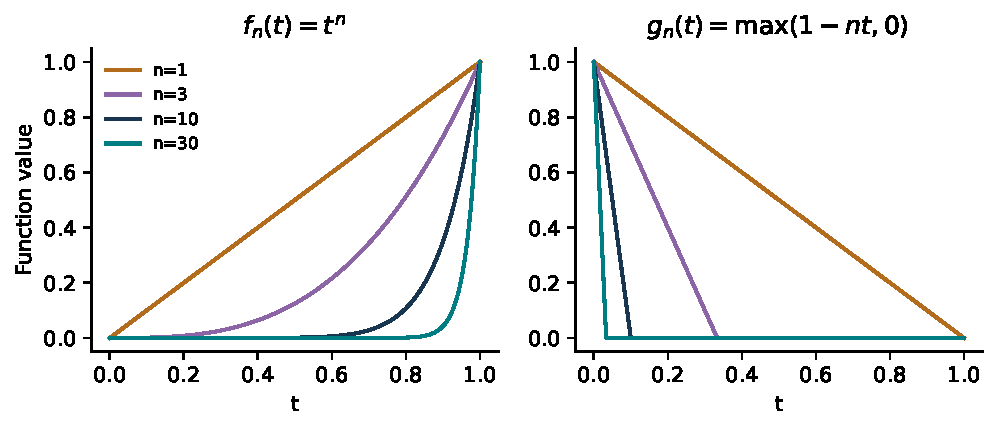
\includegraphics[width=\linewidth]{figures/function_sequences.pdf}\end{center}
On the left, the graphs $t^n$ tend pointwise to zero for $t<1$ but keep the value one at the endpoint. The pointwise limit is discontinuous. On the right, the spikes keep height one while their widths and areas shrink. Thus a small integral error does not force a small supremum error. For the spikes, only convergence in integral distance to zero is asserted; their pointwise limit at zero is one.
\end{note}


\topic{Proof clinic: Why completeness of the function space is not pointwise completeness alone}
\begin{note}{The three obligations in the proof}
A Cauchy sequence $(f_n)$ in a function space is a sequence of whole functions. To prove it converges in that space you need three separate facts:
\begin{enumerate}
\item A candidate function $f$ is defined at every input, usually using completeness of the target at each input.
\item The candidate belongs to the original space: if boundedness or continuity is part of membership, verify it.
\item The distance between $f_n$ and $f$ tends to zero in the specified metric, not merely at each input.
\end{enumerate}
In the sup metric, the uniform Cauchy hypothesis gives one cutoff valid for every input, which is strong enough for the third obligation. The $\varepsilon/3$ continuity proof handles the second obligation for continuous functions. A pointwise limit alone need not satisfy either.
\end{note}
\begin{exam}{Additional practice: diagnose an incomplete argument}
A student writes: ``For each $t$, $f_n(t)$ converges to $f(t)$. Therefore $C([0,1])$ is complete.'' Explain what must be added.
\end{exam}
\begin{answer}
One must begin with an arbitrary sequence Cauchy in the sup metric. The scalar limits define $f$, but it is still necessary to prove $f$ continuous and $\norm{f_n-f}_\infty\to0$. Pass to the limit in the uniform Cauchy bound to obtain uniform convergence. Compare the limit with one bounded term to prove boundedness. Then use uniform convergence and continuity of the approximating functions to show $f$ continuous. Without these steps, the limit might be discontinuous or the convergence might only be pointwise.
\end{answer}


\topic{Proof clinic: Constructing a useful fixed-point domain}
\begin{exam}{Additional practice: the domain makes the theorem usable}
Show $x=(x^2+1)/3$ has exactly one solution in $[0,1]$, but explain why applying the same contraction estimate on all of $\R$ fails.
\end{exam}
\begin{answer}
Let $T(x)=(x^2+1)/3$. On $[0,1]$, $1/3\le T(x)\le2/3$, so $T$ is a self-map. The interval is nonempty and complete. For $x,y\in[0,1]$,
\[|T(x)-T(y)|=\tfrac13|x-y||x+y|\le\tfrac23|x-y|.\]
The constant $2/3<1$ gives a unique fixed point in that interval by Banach. Solving the quadratic gives $x^2-3x+1=0$, so the interval solution is $(3-\sqrt5)/2$; the other root exceeds $1$.

On all of $\R$, the ratio $|T(x)-T(y)|/|x-y|=|x+y|/3$ for distinct points is unbounded, so this map is not globally Lipschitz, much less a strict contraction. The theorem on $[0,1]$ proves uniqueness in that chosen domain, not uniqueness among all real solutions.
\end{answer}
\begin{tip}
Always phrase the conclusion with its domain. A contraction can have only one fixed point in the space to which the theorem is applied; it says nothing about solutions outside that space.
\end{tip}


\topic{Worked lecture exercises}
\exercise{5.1}{Lipschitz maps and completeness}
\begin{exam}{Lecture exercise}
Prove Lipschitz maps preserve Cauchy sequences. Deduce that bi-Lipschitz metric spaces are either both complete or both incomplete.
\end{exam}
\begin{answer}
Suppose $f:E\to F$ satisfies $d_F(fx,fy)\le Ld_E(x,y)$. If $L=0$, $f$ is constant on a nonempty domain and the image of every sequence is constant, hence Cauchy. Assume $L>0$ and let $(x_n)$ be Cauchy in $E$. Given $\varepsilon>0$, choose $N$ such that $d_E(x_n,x_m)<\varepsilon/L$ for $n,m\ge N$. Then
\[d_F(fx_n,fx_m)\le Ld_E(x_n,x_m)<\varepsilon,\]
so the image sequence is Cauchy.

Now let $f$ be a bi-Lipschitz bijection and assume $E$ complete. Given Cauchy $(y_n)$ in $F$, the Lipschitz inverse makes $x_n=f^{-1}(y_n)$ Cauchy in $E$. Hence $x_n\to x\in E$. Since $f$ is Lipschitz and thus continuous, $y_n=f(x_n)\to f(x)\in F$. Thus $F$ is complete. Apply the same argument to $f^{-1}$ for the converse.
\end{answer}
\begin{tip}
For the completeness implication, start with a Cauchy sequence in the space whose completeness you need to prove. Map it to the known complete space, take a limit, and map back.
\end{tip}
\exercise{5.2}{Isometric embedding for an unbounded space}
\begin{exam}{Lecture exercise}
Show that every nonempty metric space embeds isometrically into $\ell^\infty(E;\R)$ using $j_\omega(x)(p)=d(x,p)-d(\omega,p)$ for fixed $\omega\in E$.
\end{exam}
\begin{answer}
First check that each proposed image really is a bounded function of $p$. By reverse triangle inequality,
\[|d(x,p)-d(\omega,p)|\le d(x,\omega)\quad\text{for every }p\in E.\]
The right side depends on the fixed $x$ but not on $p$, so $j_\omega(x)\in\ell^\infty(E;\R)$.

For $x,y,p\in E$, reference terms cancel:
\begin{align*}
|j_\omega(x)(p)-j_\omega(y)(p)|&=|d(x,p)-d(y,p)|\\
&\le d(x,y).
\end{align*}
Taking the supremum over $p$ gives $d_{\sup}(j_\omega(x),j_\omega(y))\le d(x,y)$. At the particular input $p=y$, the absolute difference is $|d(x,y)-d(y,y)|=d(x,y)$. Thus the supremum is also at least $d(x,y)$, proving equality. Hence $j_\omega$ is an isometry.
\end{answer}
\begin{note}{The bound need not be uniform over all image functions}
For membership, each individual function $j_\omega(x)$ must be bounded in its input $p$. There is no requirement for one common bound valid for every $x$. The whole embedded copy may be unbounded, exactly as the original space may be.
\end{note}
\exercise{5.3}{Uniqueness of completion}
\begin{exam}{Lecture exercise; the associated completion proof is marked non-examinable}
For two completions $(\widehat E_1,\iota_1)$ and $(\widehat E_2,\iota_2)$, prove there is exactly one isometry $j:\widehat E_1\to\widehat E_2$ with $j\circ\iota_1=\iota_2$, and show it is onto.
\end{exam}
\begin{answer}
Define $j_0$ on the dense subset $\iota_1(E)$ by $j_0(\iota_1(x))=\iota_2(x)$. This is well-defined because $\iota_1$ is injective. For $x,y\in E$, both embeddings preserve distance, so
\[d_2(j_0\iota_1(x),j_0\iota_1(y))=d_E(x,y)=d_1(\iota_1(x),\iota_1(y)).\]
Thus $j_0$ is isometric. Since its domain is dense and the target completion is complete, the dense Lipschitz-extension theorem gives a unique continuous extension $j$ to $\widehat E_1$, and this extension remains isometric. It satisfies $j\iota_1=\iota_2$ by construction.

To prove surjectivity, let $y\in\widehat E_2$. By density choose $x_n\in E$ with $\iota_2(x_n)\to y$. Then $(x_n)$ is Cauchy in $E$ because $\iota_2$ is isometric. Its images $\iota_1(x_n)$ are Cauchy in complete $\widehat E_1$, so converge to $z$. Continuity of $j$ gives
\[j(z)=\lim_nj(\iota_1(x_n))=\lim_n\iota_2(x_n)=y.\]
Thus $j$ is onto.

Finally any other isometry $k$ satisfying $k\iota_1=\iota_2$ agrees with $j$ on the dense subset $\iota_1(E)$. Isometries are continuous, so the identity theorem implies $k=j$. This proves the precise uniqueness statement.
\end{answer}
\exercise{5.4}{Summably controlled iterates}
\begin{exam}{Lecture exercise}
Suppose $T:E\to E$ on a nonempty complete space satisfies $d(T^nx,T^ny)\le\alpha_nd(x,y)$, where $\alpha_n\ge0$ and $\sum_{n\ge1}\alpha_n<\infty$. Prove Banach's conclusion.
\end{exam}
\begin{method}{Use a contraction iterate, or directly sum consecutive errors}
The summability implies $\alpha_n\to0$, so some iterate has constant below $1$. This gives a short proof. A direct iteration proof also explains the significance of summability.
\end{method}
\begin{answer}
Since $\sum\alpha_n$ converges with nonnegative terms, $\alpha_n\to0$. Choose $K$ with $\alpha_K<1$. Then $T^K$ is a strict contraction on the same nonempty complete space. By the contraction-iterate result, $T$ has one fixed point $p$, and $T^nx\to p$ for every starting point.

For a direct proof, set $x_n=T^nx_0$ and $D=d(x_0,Tx_0)$. For $n\ge1$,
\[d(x_n,x_{n+1})=d(T^nx_0,T^n(Tx_0))\le\alpha_nD.\]
For $m>n\ge1$, triangle inequality gives
\[d(x_n,x_m)\le D\sum_{k=n}^{m-1}\alpha_k\le D\sum_{k=n}^\infty\alpha_k\to0.\]
Thus $(x_n)$ is Cauchy and converges to $p\in E$. The $n=1$ estimate makes $T$ Lipschitz, hence continuous, so $Tp=\lim Tx_n=\lim x_{n+1}=p$. If $p,q$ are fixed, then for every $n$, $d(p,q)\le\alpha_nd(p,q)$; choose $n$ with $\alpha_n<1$ to force $p=q$. This gives existence, uniqueness and convergence.
\end{answer}
\begin{tip}
The nonnegativity of the controlling constants is the natural interpretation of Lipschitz bounds. Summability controls the whole tail, which is stronger than merely having consecutive distances tend to zero.
\end{tip}
\exercise{5.5}{Continuity of a graph parametrisation}
\begin{exam}{Lecture exercise}
For continuous $f:[a,b]\to\R$, prove $F(s)=(f(s),s)$ is continuous into $\R\times[a,b]$.
\end{exam}
\begin{answer}
Use the sum metric $D((u,s),(v,t))=|u-v|+|s-t|$. Fix $s_0\in[a,b]$ and $\varepsilon>0$. Continuity of $f$ at $s_0$ gives $\delta_1>0$ such that $|s-s_0|<\delta_1$ implies $|f(s)-f(s_0)|<\varepsilon/2$. Let $\delta=\min\{\delta_1,\varepsilon/2\}$. Then for $s\in[a,b]$ with $|s-s_0|<\delta$,
\[D(F(s),F(s_0))=|f(s)-f(s_0)|+|s-s_0|<\varepsilon.\]
Thus $F$ is continuous at arbitrary $s_0$. All standard finite-product metrics are equivalent, so the conclusion also holds for the Euclidean product metric.
\end{answer}
\exercise{5.6}{Necessary hypotheses in Cantor intersection}
\begin{exam}{Lecture exercise}
Find counterexamples when shrinking diameters or closedness is removed from Cantor's intersection theorem.
\end{exam}
\begin{answer}
Without shrinking diameters: in complete $\R$, set $F_n=[n,\infty)$. Each set is nonempty and closed; $F_{n+1}\subseteq F_n$. No real number lies in all of them, so the intersection is empty. Their diameters are infinite rather than tending to zero. For failure of uniqueness alone, the constant sequence $F_n=[0,1]$ has non-singleton intersection.

Without closedness: again in complete $\R$, take $F_n=(0,1/n)$. These sets are nonempty and nested with $\diam F_n=1/n\to0$. Their intersection is empty because any positive point is eventually excluded and zero never belongs. They are not closed.

For comparison, if completeness is omitted, take the subspace $E=(0,1)$ and $F_n=(0,1/(n+1)]$. These are closed relative to $E$, nested and shrinking, but have empty intersection. The natural limit zero is missing from $E$.
\end{answer}
\begin{tip}
When a hypothesis is removed, your counterexample must still satisfy all the others. The second example uses a complete ambient space so it isolates closedness as the failing hypothesis.
\end{tip}
\exercise{5.7}{A different Cauchy test and a separated subsequence}
\begin{exam}{Lecture exercise}
(a) Show Cauchyness is equivalent to $\forall\varepsilon>0\ \exists N\ \forall n\ge N:d(x_N,x_n)<\varepsilon$. (b) Show not Cauchy iff some subsequence has consecutive distances with positive infimum.
\end{exam}
\begin{answer}
(a) If Cauchy, choose the usual cutoff $N$ and set one index equal to $N$; the displayed condition follows. Conversely, for a target tolerance $\varepsilon>0$, apply the displayed condition with $\varepsilon/2$, obtaining $N$ with $d(x_N,x_n)<\varepsilon/2$ for all $n\ge N$. For $n,m\ge N$,
\[d(x_n,x_m)\le d(x_n,x_N)+d(x_N,x_m)<\varepsilon.\]
Thus the sequence is Cauchy.

(b) Suppose not Cauchy. Then there is $\eta>0$ such that beyond every cutoff there exist $r,s$ with $d(x_r,x_s)\ge\eta$. Start with any index $n_1$. Having chosen $n_k$, choose $r,s>n_k$ with this separation. At least one of the distances $d(x_{n_k},x_r)$, $d(x_{n_k},x_s)$ is at least $\eta/2$: if both were smaller, triangle inequality would give $d(x_r,x_s)<\eta$. Choose such an index as $n_{k+1}$. This constructs strictly increasing indices with
\[d(x_{n_k},x_{n_{k+1}})\ge\eta/2\quad\text{for every }k.\]
Hence the infimum of these consecutive subsequence distances is positive.

Conversely, if a subsequence has all consecutive distances at least $c>0$, then for every original-sequence cutoff, two sufficiently late selected consecutive terms are at distance at least $c$. This contradicts the Cauchy requirement with $\varepsilon=c$. Thus the original sequence is not Cauchy.
\end{answer}
\begin{note}{What the conclusion does and does not assert}
The proof gives separation between consecutive \emph{subsequence} terms, not necessarily between every pair of selected terms. That is exactly what this exercise requests and is already enough to disprove Cauchyness.
\end{note}
\exercise{5.8}{Optimal Lipschitz constant of integration}
\begin{exam}{Lecture exercise}
On $C([0,1])$ with sup metric, prove $R(f)=\int_0^1f$ is Lipschitz and find $\Lip R$.
\end{exam}
\begin{answer}
For any $f,g$,
\[|R(f)-R(g)|=\left|\int_0^1(f-g)\right|\le\int_0^1|f-g|\le\norm{f-g}_\infty.\]
Thus $1$ is an admissible Lipschitz constant, so $\Lip R\le1$. To prove optimality, choose $f\equiv1$, $g\equiv0$. Then $|R(f)-R(g)|=1$ while $d_{\sup}(f,g)=1$. Their ratio equals $1$, so any admissible constant must be at least $1$. Hence $\Lip R=1$.

On $[a,b]$ the same argument gives optimal constant $b-a$, with constant functions again witnessing equality.
\end{answer}
\exercise{5.9}{Uniformly continuous extension from a dense set}
\begin{exam}{Lecture exercise}
Let $A$ be dense in $E$, $F$ complete, and $f_0:A\to F$ uniformly continuous. Prove there is a unique continuous extension $f:E\to F$ and that it is uniformly continuous.
\end{exam}
\begin{method}{Separate existence, independence and regularity}
First show images of approximating Cauchy sequences converge. Then prove two choices of approximating sequences give the same image limit. Only after the function is well-defined should you prove it extends $f_0$, is uniformly continuous, and is unique.
\end{method}
\begin{answer}
For $x\in E$, density gives a sequence $a_n\in A$ with $a_n\to x$. This is Cauchy. Uniform continuity sends Cauchy sequences to Cauchy sequences: choose its global $\delta$ for a target $\varepsilon$, then use the original Cauchy property for all sufficiently late pairs. Therefore $(f_0(a_n))$ is Cauchy in complete $F$ and has a limit.

If $b_n\in A$ also tends to $x$, then $d_E(a_n,b_n)\le d_E(a_n,x)+d_E(x,b_n)\to0$. Uniform continuity implies $d_F(f_0(a_n),f_0(b_n))\to0$. The two convergent image sequences consequently have the same limit, by continuity of distance. Thus define unambiguously
\[f(x)=\lim_nf_0(a_n).\]
For $x\in A$, take the constant sequence $a_n=x$ to see $f(x)=f_0(x)$.

To prove uniform continuity, fix $\varepsilon>0$. Choose $\eta>0$ such that for $a,b\in A$,
\[d_E(a,b)<\eta\Rightarrow d_F(f_0(a),f_0(b))<\varepsilon/2.\]
Set $\delta=\eta/3$. For any $x,y\in E$ with $d_E(x,y)<\delta$, choose $a_n\to x$, $b_n\to y$ from $A$. Eventually $d_E(a_n,x)<\eta/3$ and $d_E(b_n,y)<\eta/3$, so
\[d_E(a_n,b_n)\le d_E(a_n,x)+d_E(x,y)+d_E(y,b_n)<\eta.\]
Therefore $d_F(f_0(a_n),f_0(b_n))<\varepsilon/2$. Passing to limits yields $d_F(f(x),f(y))\le\varepsilon/2<\varepsilon$. The choice $\delta$ depends only on $\varepsilon$, not on $x,y$, proving uniform continuity.

If $g$ is any continuous extension, then for $a_n\to x$ from $A$,
\[g(x)=\lim_ng(a_n)=\lim_nf_0(a_n)=f(x).\]
Thus $g=f$, proving uniqueness among continuous extensions.
\end{answer}
\begin{tip}
Continuity alone on a dense set need not preserve Cauchy sequences. This is why the uniform-continuity hypothesis is essential to this construction. The target completeness hypothesis is used at the exact point where the image Cauchy sequence needs a limit.
\end{tip}

\clearpage
\setcounter{section}{5}
\section{Sequential compactness}

\topic{Sequential compactness}
\begin{note}{Definition and first consequences}
$K\subseteq E$ is sequentially compact if \emph{every} sequence in $K$ has a subsequence converging to a point of $K$. The subsequence may depend on the starting sequence. The limit-in-$K$ condition is essential.

Sequential compactness is intrinsic: inherited distances are the same, and the required limits belong to $K$, so passing to a larger ambient space does not change it. It implies closedness, boundedness and completeness.

For closedness: if $x_n\in K$ converges to $x$ in $E$, a compactness subsequence converges to $p\in K$, and uniqueness gives $x=p$. For boundedness: if unbounded, choose points with distances from a fixed point increasing to infinity; no subsequence can converge. For completeness: a Cauchy sequence has a convergent subsequence, and the Cauchy-subsequence lemma makes the whole sequence converge.
\end{note}
\begin{note}{Closed subsets, unions and intersections}
A closed subset $F$ of a sequentially compact $K$ is sequentially compact: take a subsequence converging in $K$; closedness puts the limit in $F$. Conversely every sequentially compact subset is closed. Hence within a sequentially compact ambient space, ``closed'' and ``sequentially compact'' are equivalent for subsets.

Finite sets are sequentially compact by the infinite pigeonhole principle. Finite unions of sequentially compact sets are sequentially compact: infinitely many terms lie in one constituent. Intersections of two sequentially compact sets are sequentially compact because one is closed and the intersection is a closed subset of the other. For an arbitrary nonempty family of such sets, the same closed-subset argument works using one member to bound the intersection.
\end{note}
\begin{exam}{2022 Q4(a): compact subsets of a compact space}
Let $K$ be sequentially compact and $A\subseteq K$. Prove $A$ is sequentially compact iff $A$ is closed in $K$.
\end{exam}
\begin{answer}
Suppose $A$ is sequentially compact. If $a_n\in A$ and $a_n\to x$ in $K$, there is a subsequence $a_{n_j}\to a\in A$. Since the original sequence tends to $x$, that subsequence also tends to $x$. Uniqueness gives $x=a\in A$, proving $A$ closed in $K$.

Conversely suppose $A$ closed in $K$. Any sequence in $A$ is also a sequence in $K$, so has a subsequence converging to some $x\in K$. Since every term of the subsequence lies in $A$ and $A$ is closed in $K$, $x\in A$. Thus $A$ is sequentially compact.
\end{answer}
\begin{exam}{Additional practice: complete and bounded is insufficient}
Give a complete bounded metric space which is not sequentially compact.
\end{exam}
\begin{answer}
Take $E=\N$ with the discrete metric. Its diameter is $1$, so it is bounded. Every Cauchy sequence is eventually constant, so it is complete. But the sequence $x_n=n$ has distinct terms, as does every subsequence. A convergent sequence in a discrete space must be eventually constant, so this sequence has no convergent subsequence. Hence $E$ is not sequentially compact.
\end{answer}
\begin{tip}
Completeness controls Cauchy sequences; sequential compactness starts with \emph{any} sequence. Boundedness does not automatically produce a Cauchy subsequence in a general metric space. That extra property is total boundedness, used in the 2025 paper.
\end{tip}


\topic{Continuous images, extrema and inverse continuity}
\begin{note}{The image theorem and how to prove it}
If $f:E\to F$ is continuous and $K\subseteq E$ sequentially compact, then $f[K]$ is sequentially compact. Given $y_n\in f[K]$, choose $x_n\in K$ with $f(x_n)=y_n$. Extract $x_{n_j}\to p\in K$. Continuity gives $y_{n_j}=f(x_{n_j})\to f(p)\in f[K]$.

Therefore continuous images of sequentially compact sets are closed and bounded in \emph{any} metric codomain. A continuous real-valued function on nonempty sequentially compact $K$ attains its bounds: choose $x_n$ whose values approach the supremum, extract a convergent subsequence, then use continuity. Use $-f$ for the minimum.
\end{note}
\begin{note}{Diameter and distance are attained on compact sets}
For nonempty sequentially compact $K$, the product $K\times K$ is sequentially compact and $d$ is continuous. Thus $\diam K$ is attained at some pair $a,b\in K$. For fixed $p\in E$, $x\mapsto d(x,p)$ is continuous, so its infimum on $K$ is attained: there is $c\in K$ with $d(c,p)=\dist(p,K)$.

One can instead choose approximate minimisers $c_n$ with $d(c_n,p)<\dist(p,K)+1/n$, extract $c_{n_j}\to c\in K$, and pass to the limit.
\end{note}
\begin{note}{A continuous bijection from compact is a homeomorphism}
Let $f:K\to F$ be a continuous bijection with $K$ sequentially compact. For every closed $A\subseteq K$, $A$ is sequentially compact, so $f[A]$ is sequentially compact and hence closed in $F$. Therefore $f$ is a closed map. If $g=f^{-1}$, then $g^{-1}[A]=f[A]$ is closed for every closed $A$ in $K$, proving $g$ continuous. This is a powerful shortcut to inverse continuity.
\end{note}
\begin{exam}{2023 Q4(a): what continuous images preserve}
For continuous $f:A\to E$ with $A\subseteq\R^2$, show (a) bounded $A$ need not have bounded image; (b) closed $A$ need not have closed image; (c) closed bounded $A$ has closed bounded image.
\end{exam}
\begin{answer}
(a) Let $A=\{(t,0):0<t\le1\}$ and $f(t,0)=1/t$ into $\R$. The domain is bounded and $f$ is continuous on it, but its image $[1,\infty)$ is unbounded.

(b) Let $A=\{(t,0):t\ge0\}$ and $f(t,0)=1/(1+t)$. The domain is closed in $\R^2$ and $f$ is continuous, but its image $(0,1]$ is not closed in $\R$.

(c) If $A$ is closed and bounded in $\R^2$, Heine--Borel makes it sequentially compact. The continuous-image theorem makes $f[A]$ sequentially compact in $E$. Every such subset of a metric space is closed and bounded, giving the result. No finite-dimensional assumption is required on the target.
\end{answer}
\begin{exam}{2022 Q4(c): isometry from a compact space into itself}
If $E$ is sequentially compact and $f:E\to E$ an isometry, prove it is surjective and a homeomorphism.
\end{exam}
\begin{answer}
Fix $p\in E$. The orbit $(f^np)_{n\ge0}$ has a convergent subsequence $(f^{n_j}p)$ with strictly increasing indices. Therefore $d(f^{n_{j+1}}p,f^{n_j}p)\to0$. Since iterates are isometries,
\[d(f^{n_{j+1}-n_j}p,p)=d(f^{n_{j+1}}p,f^{n_j}p)\to0.\]
Each $n_{j+1}-n_j\ge1$, so every $f^{n_{j+1}-n_j}p$ lies in $f[E]$. The image $f[E]$ is sequentially compact (isometries are continuous), hence closed in $E$. Thus $p\in f[E]$. Since $p$ was arbitrary, $f$ is surjective.

An isometry is injective, and its inverse is isometric once surjectivity is established. Thus both directions are continuous and $f$ is a homeomorphism.
\end{answer}


\topic{Product compactness and Heine--Borel}
\begin{note}{The diagonal-subsequence construction}
For a sequence $x^{(n)}$ in a countable product of sequentially compact factors, first take a subsequence whose first coordinate converges. From that take a subsequence whose second coordinate converges. Continue, obtaining nested rows of subsequences. Select the $j$th term of row $j$.

For each fixed coordinate $i$, the diagonal tail after $i$ is a subsequence of row $i$, so that coordinate converges. The product metric's coordinatewise-convergence theorem then gives convergence of the diagonal subsequence to the tuple of coordinate limits, which belongs to the product. This proves sequential compactness for the weighted countable product metrics in the notes. Finite products need finitely many successive extractions.
\end{note}
\begin{note}{Heine--Borel in finite-dimensional norm metrics}
For $A\subseteq\R^n$ and any $\ell^p$ metric,
\[A\text{ sequentially compact}\iff A\text{ closed and bounded}.\]
For the difficult direction, boundedness puts $A$ inside a box $[-L,L]^n$. Bolzano--Weierstrass and finite product compactness show the box sequentially compact. Since $A$ is closed, it is a compact subset of the box. Norm equivalence makes the statement independent of $p$.

In particular closed balls and spheres in $\R^n$ are sequentially compact. The theorem does not extend to arbitrary metric or infinite-dimensional normed spaces by simply retaining ``closed and bounded''.
\end{note}
\begin{method}{Classify a subset of $\R^n$}
For boundedness, estimate each coordinate, or bound the norm. For closedness, use continuity of defining functions and closed preimages: e.g. $A=\{x:g(x)\le c\}$ is closed for continuous $g$. Strict inequalities often describe open sets, but intersect with other constraints carefully. If both closed and bounded, conclude sequential compactness by Heine--Borel. For nonclosedness exhibit a sequence leaving through a missing boundary point.
\end{method}
\begin{exam}{2024 Q4(b): compactness from a compact unit ball}
Let $X$ be a normed space with sequentially compact closed unit ball. Prove every closed bounded subset $A\subseteq X$ is sequentially compact.
\end{exam}
\begin{answer}
For $p\in X$ and $r>0$, the map $h(x)=p+rx$ is continuous, since $\norm{h(x)-h(y)}=r\norm{x-y}$. It sends the closed unit ball onto $B_r[p]$: one inclusion follows from $\norm{rx}\le r$, and for the reverse write $y=p+r((y-p)/r)$. Therefore every closed ball is a continuous image of a sequentially compact set and hence sequentially compact.

Since $A$ is bounded it is contained in a closed ball $B_R[0]$ for some $R>0$. It is closed in $X$, hence closed relative to that ball. A closed subset of a sequentially compact space is sequentially compact. Thus $A$ has the required property.
\end{answer}
\begin{exam}{Additional practice: classify and optimise}
Let $K=\{(x,y)\in\R^2:x^2+y^2\le4,\ y\ge0\}$. Show that $K$ is sequentially compact and find the extrema of $f(x,y)=x+y$ on $K$.
\end{exam}
\begin{answer}
The maps $(x,y)\mapsto x^2+y^2$ and $(x,y)\mapsto y$ are continuous. Their inverse images of $(-\infty,4]$ and $[0,\infty)$ are closed, so $K$ is closed. Its points satisfy $\norm{(x,y)}_2\le2$, so it is bounded. Heine--Borel gives sequential compactness.

Cauchy--Schwarz gives $x+y\le\sqrt2\sqrt{x^2+y^2}\le2\sqrt2$, attained at $(\sqrt2,\sqrt2)\in K$. Also $x\ge-2$ and $y\ge0$, so $x+y\ge-2$, attained at $(-2,0)$. Thus the minimum is $-2$ and maximum $2\sqrt2$. Compactness guarantees existence; the inequalities identify the values and attaining points.
\end{answer}


\topic{Total boundedness: the 2025 synthesis question}
\begin{note}{Definition and distinction from boundedness}
$A$ is totally bounded if for each $r>0$ it can be covered by finitely many open balls of radius $r$. The centres may lie in the ambient space, as in the 2025 paper. Boundedness gives one large ball; total boundedness requires a finite cover at \emph{every} scale.

Total boundedness implies boundedness. Fix a finite radius-$1$ cover with centres $p_1,\ldots,p_k$. For $x,y\in A$ choose covering centres $p_i,p_j$. Then
\[d(x,y)<2+\max_{i,j}d(p_i,p_j)<\infty.\]
An infinite discrete space is bounded but not totally bounded, since radius-$1/2$ balls are singletons.
\end{note}
\begin{method}{Turn finite covers into a Cauchy subsequence}
Given a sequence and a finite cover, one ball contains infinitely many \emph{terms}, so select those indices. Repeat inside that subsequence with smaller radii $1/2,1/3,\ldots$. Extract the diagonal. For each fixed stage its diagonal tail lies in a common radius-$1/j$ ball, so pairwise distances are below $2/j$. Therefore the diagonal is Cauchy. If $A$ is complete, it converges to a point of $A$.
\end{method}
\begin{exam}{2025 Q5: complete plus totally bounded}
(a) Prove total boundedness implies boundedness. (b) Given $r>0$ and a sequence in $A$, find a subsequence inside one radius-$r$ ball. (c) Prove complete and totally bounded implies sequentially compact.
\end{exam}
\begin{answer}
(a) Use a finite radius-$1$ cover. The estimate in the preceding box provides a single finite upper bound for all pairwise distances, so $A$ is bounded. If $A=\varnothing$, the assertion is immediate.

(b) A finite radius-$r$ cover exists by total boundedness. If each ball contained only finitely many sequence indices, their finite union would contain only finitely many indices, contradicting the infinitely many terms. Thus one ball contains terms at infinitely many strictly increasing indices, which form the required subsequence.

(c) Begin with an arbitrary sequence in $A$. Repeatedly apply (b), selecting nested subsequences: row $j$ lies in one radius-$1/j$ ball and is a subsequence of row $j-1$. Take the $j$th term of row $j$ as $z_j$, preserving original increasing indices. For any fixed $J$, the tail $(z_j)_{j\ge J}$ lies in the ball selected at stage $J$, so $d(z_j,z_k)<2/J$ for $j,k\ge J$. Given $\varepsilon>0$, choose $J$ with $2/J<\varepsilon$. Thus $(z_j)$ is Cauchy. Completeness of $A$ yields a limit $z\in A$. Hence every sequence has a subsequence converging in $A$, proving sequential compactness.
\end{answer}
\begin{note}{The full metric-space criterion}
Sequential compactness also implies total boundedness. If no finite radius-$r$ cover exists, recursively choose $x_{n+1}\in A\setminus\bigcup_{i\le n}B_r(x_i)$. All distinct selected points have distance at least $r$, so no subsequence can be Cauchy or convergent, contradicting compactness.

Together with completeness, this gives
\[\text{sequentially compact}\iff\text{complete and totally bounded}.\]
This explains why the infinite discrete example defeats ``complete and bounded'': it fails total boundedness.
\end{note}


\topic{Cantor space and the middle-thirds set}
\begin{note}{Two related spaces}
Cantor space is $\mathcal C=\{0,1\}^{\N}$ with metric
\[D(x,y)=\sum_{n\ge1}2^{-n}|x_n-y_n|.\]
It is sequentially compact by countable product compactness, since each factor $\{0,1\}$ is finite. Agreement on a long initial string forces small distance because the remaining tail is small.

For the Cantor middle-thirds set $Z$, begin with $Z_0=[0,1]$ and repeatedly delete the middle third of each interval. Equivalently, $Z_n=\frac13Z_{n-1}\cup(\frac13Z_{n-1}+\frac23)$, and $Z=\bigcap_nZ_n$. Stage $n$ consists of $2^n$ closed intervals of length $3^{-n}$. Thus $Z$ is closed and bounded, hence sequentially compact.
\end{note}
\begin{note}{Ternary representation and homeomorphism}
Every point of $Z$ can be written
\[\phi(c)=\sum_{n\ge1}\frac{2c_n}{3^n},\qquad c_n\in\{0,1\}.\]
Its partial sums are left endpoints of retained intervals and converge into the closed set $Z$. Conversely, for any $z\in Z$, the left endpoints of the nested stage intervals containing it give compatible digits and converge to $z$.

If two binary sequences first differ at $N$, the first differing ternary term has size $2/3^N$ while the largest possible opposing tail is $\sum_{n>N}2/3^n=1/3^N$. Therefore their images differ by at least $1/3^N>0$, proving injectivity. Also
\[|\phi(c)-\phi(d)|\le2\sum_{n\ge1}3^{-n}|c_n-d_n|\le2D(c,d).\]
So $\phi$ is a continuous bijection from sequentially compact $\mathcal C$ to $Z$, hence a homeomorphism.
\end{note}
\begin{exam}{Section 6 synthesis: large cardinality, small length}
Prove $Z$ is uncountable, nowhere dense, and has length zero in the finite-interval-cover sense used in the notes.
\end{exam}
\begin{answer}
The map $\phi:\{0,1\}^{\N}\to Z$ is bijective by the digit argument above. Since binary sequence space is uncountable by diagonalisation, $Z$ is uncountable.

Since $Z$ is closed, nowhere density is equivalent to empty interior. If a nondegenerate open interval $J$ were contained in $Z$, it would lie in every $Z_n$. Choose $n$ with $3^{-n}<|J|$. A connected interval inside a finite union of separated closed intervals must lie in one of them, but every component of $Z_n$ has length $3^{-n}<|J|$. This is impossible. Hence $\inte Z=\varnothing$ and $Z$ is nowhere dense.

For any $\varepsilon>0$, choose $n$ with $(2/3)^n<\varepsilon$. The $2^n$ retained stage-$n$ intervals cover $Z$ and have total length $2^n3^{-n}=(2/3)^n<\varepsilon$. This is exactly the length-zero condition. If open covering intervals are desired, enlarge these finitely many intervals by a total amount smaller than the remaining tolerance.
\end{answer}
\begin{tip}
Uncountable does not mean positive length or nonempty interior. For ternary endpoints such as $1/3$, the valid Cantor representation is $0.02222\ldots_3$. State ``has a ternary expansion using only $0$ and $2$'', since real-number expansions need not be unique among all ternary digits.
\end{tip}
\begin{note}{Visual explanation: the Cantor construction}
\begin{center}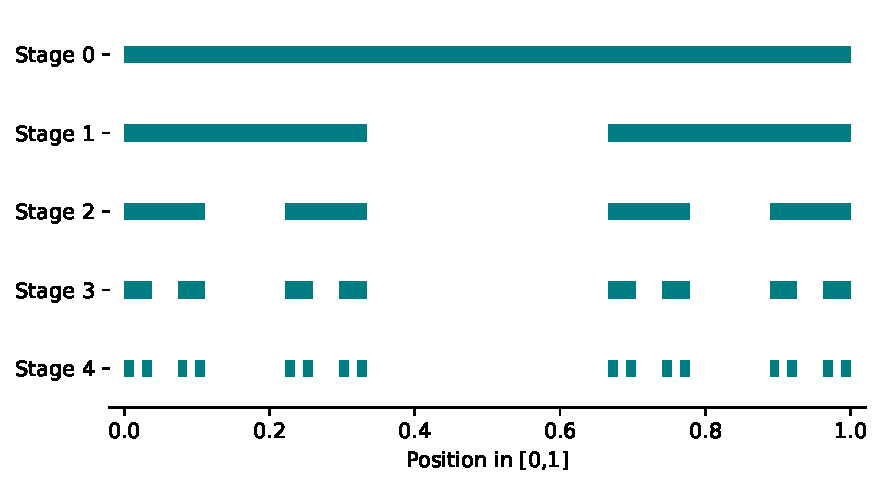
\includegraphics[width=.96\linewidth]{figures/cantor_stages.pdf}\end{center}
At stage $n$, the retained set has $2^n$ intervals, each of length $3^{-n}$. The infinite intersection is not an empty set: it includes zero, one, and every point whose ternary expansion can be chosen using only digits zero and two. The total retained length tends to zero while the final set remains uncountable.
\end{note}


\topic{Further exercise methods from the supplied notes}
\begin{note}{A convergent sequence together with its limit is closed (Exercise 6.5)}
Let $C=\{a\}\cup\{x_n:n\in\N\}$ with $x_n\to a$. For $p\notin C$, let $r=d(p,a)/3>0$. A tail lies in $B_r(a)$, so is at distance at least $2r$ from $p$. The finitely many earlier terms have a positive minimum distance from $p$. Choose a radius below both $r$ and this finite minimum; its ball about $p$ avoids $C$. Thus $E\setminus C$ is open and $C$ is closed. It is also sequentially compact: either one value occurs infinitely often, or a subsequence of the chosen sequence runs to arbitrarily late indices and hence tends to $a$.
\end{note}
\begin{note}{Cauchy tails and separated consecutive subsequence terms}
For $X_n=\{x_k:k\ge n\}$, Cauchyness is equivalent to $\diam X_n\to0$ (Exercise 6.8): each direction follows by translating ``all pairwise tail distances are small'' into the definition of diameter.

For Exercise 5.7, Cauchyness is equivalent to $\forall\varepsilon>0\ \exists N\ \forall n\ge N:d(x_N,x_n)<\varepsilon$. The reverse implication uses the triangle inequality through $x_N$ and starts with $\varepsilon/2$.

If a sequence is not Cauchy, fix $\eta>0$ witnessing this. Given a selected term $x_{n_k}$ and any later cutoff, there are two terms beyond that cutoff at distance at least $\eta$. At least one has distance at least $\eta/2$ from $x_{n_k}$; otherwise their mutual distance would be below $\eta$. Select it as $x_{n_{k+1}}$. This gives a subsequence with consecutive distances bounded below by $\eta/2$. Conversely, such a subsequence prevents Cauchyness.
\end{note}
\begin{note}{Pseudo-metrics and quotient spaces (Exercise 6.9)}
A pseudo-metric satisfies the metric axioms except that distinct points may have zero distance. Define $x\sim y$ iff $\rho(x,y)=0$. Reflexivity and symmetry are immediate; transitivity follows from $\rho(x,z)\le\rho(x,y)+\rho(y,z)=0$.

Define $d([x],[y])=\rho(x,y)$. To check well-definedness, if $x\sim x'$ and $y\sim y'$, then
\[\rho(x,y)\le\rho(x,x')+\rho(x',y')+\rho(y',y)=\rho(x',y'),\]
and the reversed inequality gives equality. Definiteness now holds for equivalence classes; other axioms descend from $\rho$.

For Riemann-integrable functions with $\rho(f,g)=\int_a^b|f-g|$, functions differing at one point can have distance zero. The quotient identifies all pairs with zero integral discrepancy, and the displayed integral defines a true metric on these classes.
\end{note}
\begin{exam}{Additional practice based on Exercise 6.9}
On $\R^2$ define $\rho((x,y),(u,v))=|x-u|$. Describe the equivalence classes and the quotient metric space.
\end{exam}
\begin{answer}
The function is a pseudo-metric, since it is the ordinary distance between first coordinates. It can vanish for distinct points such as $(0,0)$ and $(0,1)$. Two points are equivalent iff their first coordinates agree, so each class is a vertical line. Assign the class of $(x,y)$ to the real number $x$. This is a bijection from the quotient to $\R$, and the quotient distance between two classes is $|x-u|$. Thus the quotient is isometric to the usual real line.
\end{answer}
\begin{note}{One remaining set-theoretic construction (Exercise 4.12)}
Given $c=(c_n)\in\{0,1\}^{\N}$, put $x=\sum_{n\ge1}c_n10^{-n}$. Then $\lfloor10^nx\rfloor=\sum_{k=1}^nc_k10^{n-k}$ because the remaining tail is at most $1/9<1$. All terms except $c_n$ are even; hence the parity of this floor is $c_n$. Therefore the parity-of-decimal-floors map in Exercise 4.12 is surjective onto binary sequence space. Any surjection $\N\to\R$ composed with it would enumerate binary sequence space, contradicting diagonalisation. Here the floor uses integers, including negative integers, as usual.
\end{note}


\topic{Detailed proof: Compact domain makes continuity uniform}
\begin{exam}{Additional practice based on Section 2}
Let $K$ be a sequentially compact metric space and $f:K\to F$ continuous into a metric space. Prove $f$ uniformly continuous.
\end{exam}
\begin{method}{Negate the global claim to obtain two close-input sequences}
Failure of uniform continuity gives one output tolerance that cannot be achieved by any single input tolerance. Choosing input tolerance $1/n$ produces pairs of inputs which are increasingly close but whose outputs remain a fixed distance apart.
\end{method}
\begin{answer}
Suppose $f$ is not uniformly continuous. Then there is $\varepsilon_0>0$ such that, for every $\delta>0$, some $x,y\in K$ satisfy $d_K(x,y)<\delta$ but $d_F(f(x),f(y))\ge\varepsilon_0$. For each $n$ choose such $x_n,y_n$ with
\[d_K(x_n,y_n)<1/n,\qquad d_F(f(x_n),f(y_n))\ge\varepsilon_0.\]
Sequential compactness gives a subsequence $x_{n_j}\to p\in K$. Then
\[d_K(y_{n_j},p)\le d_K(y_{n_j},x_{n_j})+d_K(x_{n_j},p)\to0,\]
so $y_{n_j}\to p$ too. Continuity at $p$ implies $f(x_{n_j})\to f(p)$ and $f(y_{n_j})\to f(p)$. Consequently
\[d_F(f(x_{n_j}),f(y_{n_j}))\le d_F(f(x_{n_j}),f(p))+d_F(f(p),f(y_{n_j}))\to0.\]
But these distances are all at least $\varepsilon_0>0$, a contradiction. Thus $f$ is uniformly continuous.
\end{answer}
\begin{tip}
Compactness is applied only to the first sequence. The closeness of each input pair then forces the corresponding second subsequence to have the same limit. Independently extracting two subsequences could lose the required pairing.
\end{tip}


\topic{Proof clinic: Completeness and compactness: keep the logical arrows separate}
\begin{note}{A complete space need not keep every sequence under control}
Completeness only promises limits for Cauchy sequences. In $\R$, the sequence $n$ has no convergent subsequence, but this does not contradict completeness because it is not Cauchy. Sequential compactness demands a convergent subsequence from \emph{any} sequence, so it is stronger.

In $\R^n$, boundedness is strong enough, via Bolzano--Weierstrass, to obtain a convergent subsequence in the ambient space. Closedness then retains the limit inside the subset. In general metric spaces, boundedness alone does not give that subsequence; total boundedness is what provides successively finer finite covers.

Thus two routes to sequential compactness are available: in finite-dimensional norm metrics, closed and bounded; in general metric spaces, complete and totally bounded. Do not silently use the finite-dimensional route outside its hypotheses.
\end{note}
\begin{exam}{Additional practice: classification table}
Classify $\R$, $(0,1)$, $[0,1]$ and an infinite discrete space for completeness, boundedness and sequential compactness.
\end{exam}
\begin{answer}
\begin{tabular}{p{.32\linewidth}ccc}
\textbf{Usual metric unless stated} & \textbf{Complete} & \textbf{Bounded} & \textbf{Seq. compact}\\[4pt]
$\R$ & Yes & No & No\\[3pt]
$(0,1)$ & No & Yes & No\\[3pt]
$[0,1]$ & Yes & Yes & Yes\\[3pt]
Infinite discrete space & Yes & Yes & No
\end{tabular}

For $\R$, use its completeness theorem and the sequence $n$ to disprove compactness. For $(0,1)$, $1/n$ (starting at $n=2$) is Cauchy but its only ambient limit is missing. For $[0,1]$, use closedness and completeness, then Heine--Borel. For the discrete example, Cauchy sequences are eventually constant but a sequence of distinct points has no convergent subsequence.
\end{answer}


\topic{Proof clinic: Recognising when an infimum becomes an attained minimum}
\begin{exam}{Additional practice: when a distance infimum is attained}
In the metric space $E=(0,\infty)$ with usual metric, let $A=(0,1]$ and $p=2$. Find the nearest point. Then in $E=\R$, give a nonclosed set with a finite unattained point-distance infimum.
\end{exam}
\begin{answer}
For the first case, $d(2,a)=2-a\ge1$ for $0<a\le1$, with equality at $a=1$. Thus $\dist(2,A)=1$ and it is attained. This shows compactness is sufficient for attainment, not necessary in every particular example.

For the requested unattained infimum in $\R$, let $B=(0,1)$ and $p=2$. Then $d(2,b)=2-b>1$ for every $b\in B$. Taking $b_n=1-1/n$ for $n\ge2$ gives distances $1+1/n\to1$. Hence $\dist(2,B)=1$ and no point attains it. The missing endpoint prevents attainment.
\end{answer}
\begin{note}{A stronger warning in a general metric space}
Even closedness alone need not guarantee a nearest point. On $E=\{p,a_1,a_2,\ldots\}$ define $d(p,a_n)=1+1/n$, $d(a_n,a_m)=2$ for distinct $n,m$, and zero on the diagonal. This is a metric: the only potentially smaller two-leg route between distinct $a_n,a_m$ through $p$ has length $2+1/n+1/m>2$; routes from $p$ via another $a_m$ are longer than its direct distances. The subset $A=\{a_n:n\ge1\}$ is closed because $B_1(p)$ avoids it. Yet $\dist(p,A)=1$ is not attained. The set is not sequentially compact, since its points are uniformly separated. This is why the compact attainment theorem carries more information than closedness alone.
\end{note}


\topic{Proof clinic: Two different diagonal arguments}
\begin{note}{Do not confuse construction with extraction}
Cantor's uncountability diagonal changes the $n$th coordinate of the $n$th listed object to produce a new object absent from a proposed list. The purpose is to show no enumeration can be exhaustive.

The compact-product diagonal extracts the $n$th term of the $n$th \emph{nested subsequence}. It produces a subsequence whose tail inherits convergence in every fixed coordinate. The purpose is to make infinitely many coordinate requirements hold simultaneously.

Both inspect a diagonal array, but their logical jobs differ. In the second argument, the rows must be nested subsequences. Taking a diagonal from unrelated convergent coordinate sequences does not necessarily produce a subsequence of the original product sequence.
\end{note}
\begin{exam}{Additional practice: a compact-product sequence}
In $\{0,1\}^{\N}$ with $D(x,y)=\sum_i2^{-i}|x_i-y_i|$, let $x^{(n)}$ have its first $n$ coordinates equal to $1$ and the rest zero. Find its limit and the exact distance to it.
\end{exam}
\begin{answer}
The candidate limit is $a=(1,1,1,\ldots)$. For each fixed coordinate $i$, $x_i^{(n)}=1$ once $n\ge i$, so coordinatewise convergence holds. Directly,
\[D(x^{(n)},a)=\sum_{i>n}2^{-i}=2^{-n}\to0.\]
Thus the sequence converges to $a$ in the weighted product metric. In contrast, its unweighted sup distance from $a$ is $1$ for every $n$, because there are always later coordinates still equal to zero. The metric determines which kind of convergence is being discussed.
\end{answer}


\topic{Worked lecture exercises}
\exercise{6.1}{Finite sets, unions and intersections}
\begin{exam}{Lecture exercise}
Show finite sets are sequentially compact and the union and intersection of two sequentially compact sets are sequentially compact.
\end{exam}
\begin{answer}
If $A$ is finite and $(x_n)$ a sequence in $A$, some point $a\in A$ occurs infinitely often by the infinite pigeonhole principle. Select its indices in increasing order to get a constant subsequence, which converges to $a\in A$. Thus finite sets are sequentially compact. The empty case is vacuous.

Let $A,B$ sequentially compact and $(x_n)$ a sequence in $A\cup B$. Either infinitely many terms lie in $A$, or only finitely many do, in which case infinitely many lie in $B$. Select a subsequence lying entirely in one constituent. Its sequential compactness gives a further subsequence converging to a point of that constituent, hence of $A\cup B$. Therefore the union is sequentially compact.

For the intersection, start with a sequence in $A\cap B$. Since it lies in $A$, choose a subsequence converging to $a\in A$. Sequentially compact $B$ is closed in the ambient metric space. All selected terms lie in $B$, so their limit $a$ lies in $B$ too. Hence $a\in A\cap B$, proving sequential compactness of the intersection.
\end{answer}
\begin{tip}
The intersection argument uses closedness of one compact set. It is unnecessary to extract a second subsequence, although that alternative also works with uniqueness of limits.
\end{tip}
\exercise{6.2}{A closest point in a compact set}
\begin{exam}{Lecture exercise}
For nonempty sequentially compact $K$ and $p\in E$, prove there exists $c\in K$ with $d(c,p)=\dist(p,K)$.
\end{exam}
\begin{answer}
Let $r=\dist(p,K)=\inf_{x\in K}d(p,x)$. It is a finite nonnegative real because $K$ is nonempty and distances are finite. By infimum approximation choose $x_n\in K$ such that
\[r\le d(p,x_n)<r+1/n.\]
Then $d(p,x_n)\to r$. Sequential compactness gives a subsequence $x_{n_j}\to c\in K$. Reverse triangle inequality shows $|d(p,x_{n_j})-d(p,c)|\le d(x_{n_j},c)\to0$, so this subsequence of distance values tends to $d(p,c)$. It also tends to $r$, since the whole distance sequence does. Uniqueness of real limits gives $d(p,c)=r$, as required.
\end{answer}
\begin{method}{Approximate, extract, pass to the limit}
This three-step pattern proves many attainment theorems. The infimum first gives approximate minimisers; compactness gives a convergent subsequence; continuity turns its limiting value into an actual minimiser.
\end{method}
\exercise{6.3}{Continuous functions attain extrema}
\begin{exam}{Lecture exercise}
For continuous $f:E\to\R$ and nonempty sequentially compact $K\subseteq E$, prove $f$ attains its maximum and minimum on $K$.
\end{exam}
\begin{answer}
First $f[K]$ is sequentially compact by the continuous-image theorem, and hence bounded. Therefore $s=\sup f[K]$ and $l=\inf f[K]$ are finite reals.

By supremum approximation choose $x_n\in K$ with $s-1/n<f(x_n)\le s$. Thus $f(x_n)\to s$. Sequential compactness supplies $x_{n_j}\to q\in K$. Continuity gives $f(x_{n_j})\to f(q)$. Since the same subsequence of values tends to $s$, uniqueness yields $f(q)=s$. Thus the supremum is attained.

Apply the same argument to $-f$, which is continuous. It has a maximiser $p\in K$. Then $-f(x)\le-f(p)$ for all $x\in K$, which means $f(p)\le f(x)$. Therefore
\[f(p)\le f(x)\le f(q)\quad\text{for all }x\in K.\]
\end{answer}
\begin{tip}
Nonemptiness is needed for attaining points. The empty set is sequentially compact but supplies neither a maximiser nor a minimiser.
\end{tip}
\exercise{6.4}{Bounded means fitting inside a box}
\begin{exam}{Lecture exercise}
For $A\subseteq\R^N$, prove boundedness in $d_\infty$ iff $A\subseteq[-L,L]^N$ for some finite $L\ge0$.
\end{exam}
\begin{answer}
If $A=\varnothing$, choose $L=0$. Assume $A\ne\varnothing$ and $\diam_\infty A=D<\infty$. Choose $a\in A$. For each $x\in A$,
\[\norm{x}_\infty\le\norm{x-a}_\infty+\norm{a}_\infty\le D+\norm{a}_\infty.\]
Set $L=D+\norm{a}_\infty$. Since every coordinate has modulus at most $\norm{x}_\infty\le L$, $x\in[-L,L]^N$, proving containment.

Conversely, if every coordinate of every point has modulus at most $L$, then for $x,y\in A$ each coordinate difference satisfies $|x_i-y_i|\le2L$. Taking the maximum gives $d_\infty(x,y)\le2L$, so $\diam_\infty A\le2L<\infty$. Thus $A$ is bounded.
\end{answer}
\exercise{6.5}{A convergent sequence with its limit is closed}
\begin{exam}{Lecture exercise}
If $x_n\to a$ in $E$, prove $C=\{a\}\cup\{x_n:n\in\N\}$ is closed.
\end{exam}
\begin{method}{Separate the tail from the finite beginning}
For a point $p\notin C$, the limit $a$ is at positive distance from $p$. Late terms cluster near $a$, leaving room around $p$. Only finitely many early terms remain to avoid.
\end{method}
\begin{answer}
Fix $p\in E\setminus C$. Since $p\ne a$, let $r=d(p,a)/3>0$. Choose $N$ such that $d(x_n,a)<r$ for all $n\ge N$. Reverse triangle inequality gives
\[d(p,x_n)\ge d(p,a)-d(a,x_n)>3r-r=2r\quad(n\ge N).\]
Every early term is distinct from $p$, so all distances $d(p,x_i)$ for $i<N$ are positive. Define
\[s=\min\bigl(\{r\}\cup\{d(p,x_i)/2:1\le i<N\}\bigr)>0.\]
A point within distance $s$ of $p$ cannot equal $a$, since $d(p,a)=3r>s$; cannot equal a tail term, since those have distance above $2r\ge2s$; and cannot equal an early term, since its distance is at least $2s$. Hence $B_s(p)\cap C=\varnothing$. Thus every point outside $C$ has a ball outside $C$, so the complement is open and $C$ is closed.
\end{answer}
\exercise{6.6}{Composition of continuous maps}
\begin{exam}{Lecture exercise}
For continuous $f:E\to F$ and $g:F\to G$, prove $g\circ f$ continuous.
\end{exam}
\begin{answer}
Fix $p\in E$ and $\varepsilon>0$. By continuity of $g$ at $f(p)$ there is $\eta>0$ such that $d_F(y,f(p))<\eta$ implies $d_G(g(y),g(f(p)))<\varepsilon$. By continuity of $f$ at $p$ there is $\delta>0$ such that $d_E(x,p)<\delta$ implies $d_F(f(x),f(p))<\eta$. Combining the two implications gives
\[d_E(x,p)<\delta\Rightarrow d_G(g(f(x)),g(f(p)))<\varepsilon.\]
Thus the composition is continuous at arbitrary $p$.

Equivalently, for open $U\subseteq G$, $(g\circ f)^{-1}[U]=f^{-1}[g^{-1}[U]]$ is open because each inverse-image step preserves openness.
\end{answer}
\begin{tip}
Choose tolerances in reverse order: first what $g$ needs in its input, then what $f$ needs to achieve that tolerance. This is why $\eta$ is selected before $\delta$.
\end{tip}
\exercise{6.7}{The identity theorem}
\begin{exam}{Lecture exercise}
For continuous $f,g:E\to F$, prove their agreement set is closed. Deduce that agreement on a dense subset implies agreement everywhere.
\end{exam}
\begin{answer}
Let $H=\{x\in E:f(x)=g(x)\}$. Take a sequence $x_n\in H$ converging in $E$ to $x$. Then continuity gives $f(x_n)\to f(x)$ and $g(x_n)\to g(x)$. Since $f(x_n)=g(x_n)$ for every $n$, these are the same sequence; uniqueness of limits in $F$ gives $f(x)=g(x)$. Therefore $x\in H$, proving $H$ closed.

Now suppose $D$ is dense in $E$ and $f=g$ on $D$. Then $D\subseteq H$, so closure monotonicity gives $E=\cl D\subseteq\cl H=H$. Since $H\subseteq E$ already, $H=E$. Thus $f=g$ on all of $E$.
\end{answer}
\begin{note}{Where you use this result}
It supplies uniqueness of continuous extensions from dense sets, including the extension theorem and uniqueness of completion maps. The values on a dense set determine a continuous function everywhere.
\end{note}
\exercise{6.8}{Diameters of tails}
\begin{exam}{Lecture exercise}
For $X_n=\{x_k:k\ge n\}$, prove $(x_n)$ is Cauchy iff $\diam X_n\to0$.
\end{exam}
\begin{answer}
Assume Cauchy and fix $\varepsilon>0$. Choose $N$ such that $d(x_j,x_k)<\varepsilon/2$ for $j,k\ge N$. Every pair in $X_N$ satisfies this, so taking a supremum gives $\diam X_N\le\varepsilon/2$. Since $X_n\subseteq X_N$ for $n\ge N$, diameter monotonicity gives $\diam X_n\le\varepsilon/2<\varepsilon$ for $n\ge N$. Thus the tail diameters tend to zero.

Conversely, suppose $\diam X_n\to0$. Given $\varepsilon>0$, choose $N$ with $\diam X_N<\varepsilon$. For $j,k\ge N$, both $x_j,x_k\in X_N$, so $d(x_j,x_k)\le\diam X_N<\varepsilon$. This is exactly Cauchyness.
\end{answer}
\begin{tip}
An infinite supremum of numbers strictly below $\varepsilon$ may equal $\varepsilon$. Starting with $\varepsilon/2$ makes the first implication's strict final bound safe.
\end{tip}
\exercise{6.9}{Turning a pseudo-metric into a metric}
\begin{exam}{Lecture exercise}
Let $\rho$ satisfy all metric axioms except that zero need not force equality. Prove $x\sim y$ iff $\rho(x,y)=0$ is an equivalence relation, and $d([x],[y])=\rho(x,y)$ is a well-defined metric. Interpret this for integral discrepancy on Riemann-integrable functions.
\end{exam}
\begin{method}{Well-definedness must precede metric axioms}
A point of the quotient is an equivalence class, which has many possible representatives. Before declaring a distance, prove that changing either representative does not change the formula's value.
\end{method}
\begin{answer}
Reflexivity holds because $\rho(x,x)=0$. Symmetry follows from $\rho(x,y)=\rho(y,x)$. If $x\sim y$ and $y\sim z$, triangle inequality gives $0\le\rho(x,z)\le\rho(x,y)+\rho(y,z)=0$, so $x\sim z$. Thus $\sim$ is an equivalence relation.

If $x\sim x'$ and $y\sim y'$, then
\[\rho(x,y)\le\rho(x,x')+\rho(x',y')+\rho(y',y)=\rho(x',y').\]
Interchanging primed and unprimed points gives the reverse inequality, hence equality. The formula for $d$ is therefore independent of representatives.

Its values are finite and nonnegative. It is symmetric because $\rho$ is. Also $d([x],[y])=0$ iff $x\sim y$ iff $[x]=[y]$, giving definiteness on classes. For any third class $[z]$,
\[d([x],[z])=\rho(x,z)\le\rho(x,y)+\rho(y,z)=d([x],[y])+d([y],[z]).\]
Thus it is a metric.

For Riemann-integrable functions on a nondegenerate $[a,b]$, $\rho(f,g)=\int_a^b|f-g|$ is a pseudo-metric. For example $f\equiv0$ and $g$ equal to $1$ at one point and $0$ elsewhere are distinct with zero discrepancy. The quotient identifies all functions whose absolute difference has integral zero; the distance between their classes is that integral. It is now a true metric because zero distance means equality of classes, not equality at every input.
\end{answer}
\begin{tip}
Do not confuse a quotient class with a chosen function. The quotient construction deliberately treats some different pointwise functions as the same point, repairing the failed definiteness axiom.
\end{tip}

\topic{Past-paper navigation and source register}
\begin{note}{2022 paper: where to revise each question}
\begin{tabular}{p{.18\linewidth}p{.73\linewidth}}
Q1 & Balls, isometries and Lipschitz maps: four equidistant planar points.\\[3pt]
Q2(a)--(b) & Open sets and interior: definition and unions of open/closed balls.\\[3pt]
Q2(c)--(d) & Metric subspaces and relative topology: restricted metric and relative-open-set proof.\\[3pt]
Q3(a)--(b) & Completeness and closed subspaces: definitions, homeomorphism and uniform-continuity transfer.\\[3pt]
Q3(c) & Banach theorem and contraction iterates: complete model proof.\\[3pt]
Q4(a)--(b) & Sequential compactness and continuous images.\\[3pt]
Q4(c) & Continuous images, extrema and inverse continuity: compact self-isometry.
\end{tabular}
\end{note}
\begin{note}{2023 paper: where to revise each question}
\begin{tabular}{p{.18\linewidth}p{.73\linewidth}}
Q1 & Discrete metric and equilateral three-point embedding.\\[3pt]
Q2(a) & Norms, norm-induced metrics and the matrix norm model answer.\\[3pt]
Q2(b) & Closed sets, closure and boundary: closure of finite unions and intersection counterexample.\\[3pt]
Q2(c) & Continuity: definition, open-preimage theorem, constant-image counterexample.\\[3pt]
Q3(a) & Density: dense intersect open dense, and disjoint dense counterexample.\\[3pt]
Q3(b) & Function metrics and completeness of sup spaces.\\[3pt]
Q4(a) & Continuous images: bounded/closed counterexamples and Heine--Borel.\\[3pt]
Q4(b) & Finite and countable products: weighted sup metric, full model proof.
\end{tabular}
\end{note}
\begin{note}{2024 paper: where to revise each question}
\begin{tabular}{p{.18\linewidth}p{.73\linewidth}}
Q1 & Discrete metric, exact ball radii, eventual constancy.\\[3pt]
Q2(a)--(c) & Open sets, complements, subspaces, relative clopen example.\\[3pt]
Q2(d)(i)--(iv) & Open unions, infinite-intersection counterexample, density.\\[3pt]
Q2(d)(v) & Countable dense dyadic polygonal family in $C([0,1])$.\\[3pt]
Q3(a)--(c) & Equivalent metrics: Cauchy equivalence, truncation and arctangent.\\[3pt]
Q3(d) & Completeness of $\ell^\infty(S;[0,1])$.\\[3pt]
Q4(a) & Sequential compactness, image theorem, bounded sets in balls.\\[3pt]
Q4(b) & Product compactness and Heine--Borel: compact unit ball argument.
\end{tabular}
\end{note}
\begin{note}{2025 paper: where to revise each question}
\begin{tabular}{p{.18\linewidth}p{.73\linewidth}}
Q1 & Triangle estimates: full four-point and reverse-triangle arguments.\\[3pt]
Q2 & Countability: definition and binary diagonal proof.\\[3pt]
Q3(a)--(d) & Open/closed/continuous definitions, openness of balls, disjoint balls and proper open set.\\[3pt]
Q3(e)--(f) & Closed complement proof and inverse-open-set characterisation.\\[3pt]
Q4(a) & Completeness iff closedness in a complete ambient space.\\[3pt]
Q4(b) & Complete continuous-function space: bounded image plus uniform limits.\\[3pt]
Q5 & Total boundedness: all three parts worked immediately after the topic.
\end{tabular}
\end{note}
\begin{note}{Source register and coverage}
The following twelve supplied PDFs and the recovered original Section 1 PDF were used. Page references here are physical PDF pages, not the miniature slide numbers printed within pages.
\begin{enumerate}
\item \texttt{MS+T.Section0}: 8 PDF pages. Metric axioms and examples; Exercises 0.1--0.6.
\item \texttt{MS+T.Section1.singleSB}: 26 pages, recovered from the earlier upload dated 15 October 2026. Sets, functions, equivalence relations, countability and optional order theory; Exercises 1.1--1.19.
\item \texttt{MS+T.Section2}: 27 pages. Real analysis, linear algebra, continuity and integration; Exercises 2.1--2.10.
\item \texttt{MS+T.Section3}: 15 pages. Metrics, balls, Lipschitz maps, boundedness, sequences and function spaces; Exercises 3.1--3.14.
\item \texttt{MS+T.Section4}: 17 pages. Topology, density, continuity, subspaces, metric equivalence and products; Exercises 4.1--4.12.
\item \texttt{MS+T.Section5}: 16 pages. Completeness, extensions, completion, Banach, integral equations, Cantor intersection and Baire; Exercises 5.1--5.9.
\item \texttt{MS+T.Section6}: 11 pages. Sequential compactness, products, Heine--Borel and Cantor set; Exercises 6.1--6.9.
\item \texttt{MTS.AppendixOne.ProofOfMinkowski.Inequality}: 3 pages, non-examinable.
\item \texttt{MTS.AppendixTwo.LipschitzExtensionTheorem}: 2 pages, non-examinable.
\item \texttt{MATH316Exam2022.pdf}: 3 pages; all four main questions mapped above.
\item \texttt{MATH316.pdf}: the 2023 paper, 6 pages including information sheet; all four main questions mapped above.
\item \texttt{MATH316MetricSpacesMainSummer2024.pdf}: 6 pages including information sheet; all four main questions mapped above.
\item \texttt{2024-25.FinalisedMATH316.Exam.pdf}: the 2025 paper, 6 pages including information sheet; all five main questions mapped above.
\end{enumerate}
The narrative consolidates repeated definitions and results. The numbered exercise workbooks added to this edition give solutions to all 79 exercises in the Sections 0--6. Non-examinable and optional material retains its status. The guide is a teaching resource, not an official solution manual.
\end{note}
\begin{tip}
Before an exam, reproduce the definition boxes without looking. Practise the open-ball, complement, relative-open-set, dense-intersection, sup-space completeness, uniform-limit, Banach and continuous-image proofs. Then do the four papers under the actual instructions on each paper. Their recurring topics guide practice priorities, but do not establish what a future paper will ask.
\end{tip}


\appendix
\renewcommand{\thesection}{\Roman{section}}
\titleformat{\section}{\Large\bfseries}{Appendix \thesection}{1em}{}
\renewcommand{\thesubsection}{\Roman{section}.\arabic{subsection}}
\clearpage
\section{Minkowski Inequality}
\begin{note}{Appendix I: convexity and Minkowski, following the supplied proof}
A function $f$ on an interval is convex if
\[f((1-t)a+tb)\le(1-t)f(a)+tf(b)\quad(0<t<1).\]
For differentiable $f$, a nondecreasing derivative implies convexity: use the mean value theorem on the two subintervals about an intermediate point to compare secant slopes. Continuity extends the inequality to included endpoints. In particular $u\mapsto|u|^p$ is convex for $p\ge1$.

A subset of a vector space is convex if it contains the line segment between every two of its points. Linear images, translates, and closures of convex sets are convex; norm balls are convex. Coordinatewise convexity gives, when $\norm{x}_p,\norm{y}_p\le1$,
\[\sum_i|(1-t)x_i+ty_i|^p\le(1-t)\sum_i|x_i|^p+t\sum_i|y_i|^p\le1.\]
Thus the $\ell^p$ unit ball is convex. For nonzero $x,y$, set $a=\norm{x}_p$, $b=\norm{y}_p$, $\widehat x=x/a$, $\widehat y=y/b$. Then
\[\frac{x+y}{a+b}=\frac a{a+b}\widehat x+\frac b{a+b}\widehat y\]
is in that unit ball. Homogeneity gives $\norm{x+y}_p\le a+b$, which is Minkowski. Zero-vector cases are immediate; $p=\infty$ follows coordinatewise. For complex vectors, use $|x_i+y_i|\le|x_i|+|y_i|$ then real Minkowski on the nonnegative modulus vectors.
\end{note}
\begin{exam}{Appendix I practice, not an exam prediction}
Use convexity of the unit ball to prove the triangle inequality for $\ell^p$.
\end{exam}
\begin{answer}
If either vector is zero, the inequality is equality. Otherwise write $a=\norm{x}_p>0$, $b=\norm{y}_p>0$. The normalised vectors $x/a,y/b$ lie in the unit ball. Their convex combination with weights $a/(a+b)$ and $b/(a+b)$ is $(x+y)/(a+b)$, so its norm is at most $1$. Multiply by $a+b$ to obtain $\norm{x+y}_p\le\norm{x}_p+\norm{y}_p$. Convexity of the ball was proved using convexity of $|\cdot|^p$, without assuming the triangle inequality under proof.
\end{answer}

\clearpage
\section{Lipschitz Extension Theorem}
\begin{note}{Appendix II: extension from a set that need not be dense}
For continuous real-valued functions on a closed subset of a metric space, Tietze's theorem gives a continuous extension, preserving bounds when bounded. The supplied appendix treats this as non-examinable.

For $f:A\to\R$ with Lipschitz constant $L$, at one new point $p$ the permitted value $z$ must satisfy
\[\sup_{a\in A}(f(a)-Ld(p,a))\le z\le\inf_{a\in A}(f(a)+Ld(p,a)).\]
The interval is nonempty, since for $a,b\in A$,
\[f(a)-f(b)\le Ld(a,b)\le Ld(a,p)+Ld(p,b).\]
The appendix extends one point at a time and uses Zorn's lemma to obtain a maximal extension, which must have full domain. The optimal Lipschitz constant remains $L$ because restriction already attains its supremal ratio.

An alternative explicit real-valued extension for nonempty $A$ is
\[F(x)=\inf_{a\in A}\{f(a)+Ld(x,a)\}.\]
It is finite: fixing $a_0\in A$, the expression is bounded below by $f(a_0)-Ld(x,a_0)$ and above by $f(a_0)+Ld(x,a_0)$. On $A$ the Lipschitz inequality and the choice $a=x$ give $F=f$. Triangle inequality gives $F(x)\le F(y)+Ld(x,y)$ and the reverse, proving $L$-Lipschitz continuity. Unlike dense extension, extension from a nondense set need not be unique. The real-valued target assumption matters.
\end{note}
\begin{exam}{Appendix II practice: range of possible values}
For $A=\{0,2\}\subset\R$, $f(0)=0$, $f(2)=2$, which values at $1$ permit a $1$-Lipschitz extension? What if $A=\{0\}$ and we allow constant at most $1$?
\end{exam}
\begin{answer}
For the first case, the value $z$ must satisfy $|z|\le1$ and $|z-2|\le1$. Hence $z\in[-1,1]\cap[1,3]=\{1\}$. In the second case the sole requirement is $|z|\le1$, so every $z\in[-1,1]$ works on $\{0,1\}$. For example $F(x)=x$, $F(x)=-x$ and $F(x)=0$ are different extensions with Lipschitz constant at most $1$. This illustrates that nondensity can allow nonuniqueness; it does not assert that the optimal constant of the original singleton map is $1$ (it is $0$).
\end{answer}
\end{document}
